\label{sec:EfficiencyAppendix}
\addtocontents{toc}{\protect\setcounter{tocdepth}{0}}
\section{Isolated-photon efficiency}

We report correlation functions that are normalized per photon trigger so the photon efficiency cancels. In principle, we might introduce a bias if the photon efficiency varied rapidly within the photon \pt~range that we are using (12--40 \GeVc). Here we show that this is not the case.  

The efficiency our our isolated-photon selection is shown in Figure~\ref{fig:photonEff_pPb}. The efficiency is rather independent of \pt~in the range relevant for this analysis. We observe less than 1\% variation between the high and low of the energy range of our photon triggers (77.7\% at 12 \GeVc~and 78.5\% at 40 \GeVc). This level of variation has a negligible impact in our correlation analysis. 
\begin{figure}
\centering
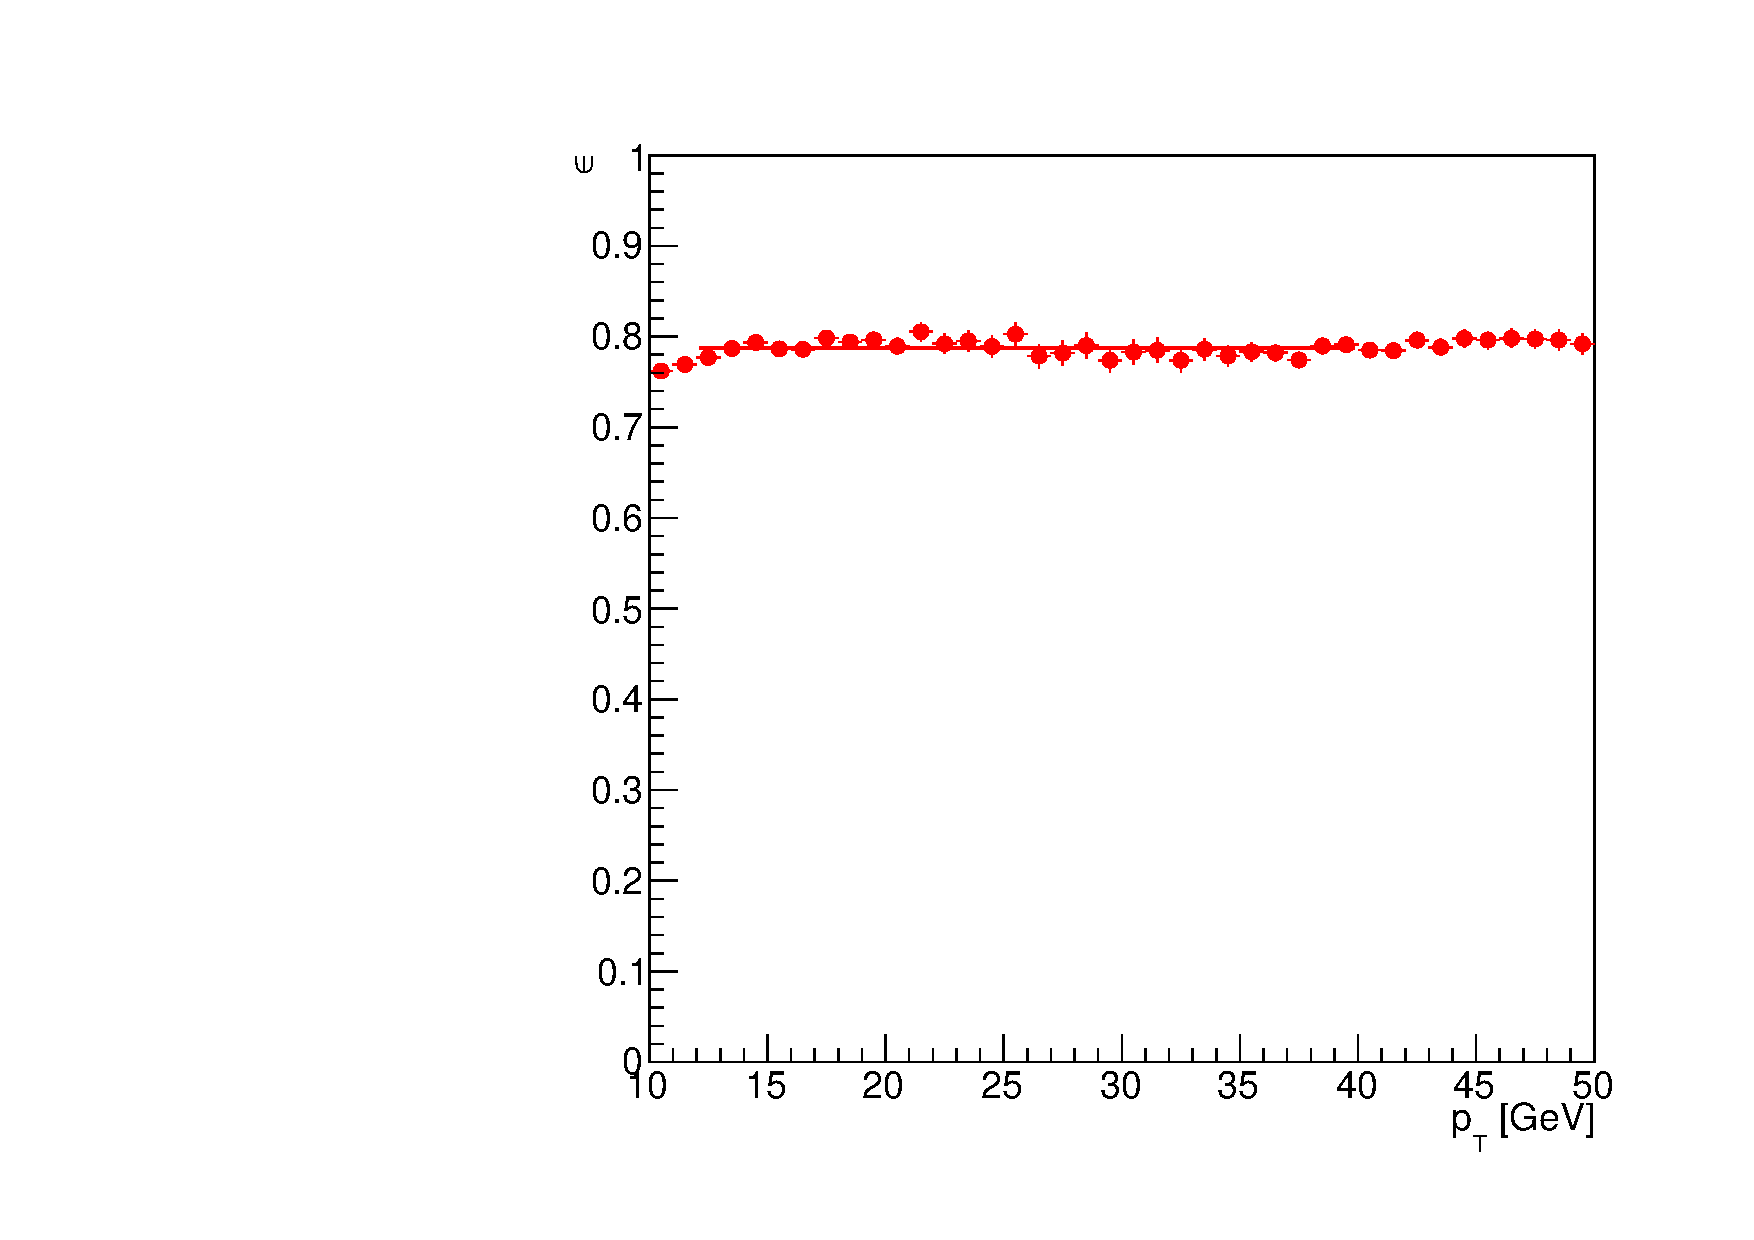
\includegraphics[width=0.45\textwidth]{EfficiencyAppendix/Efficiency_photon_pPb.pdf}
\caption{Isolated-photon efficiency obtained with \pPb~simulation.}
\label{fig:photonEff_pPb}
\end{figure}

\section{Checks of UE estimates with standard tracking }
As discussed in Section~\ref{sec:tracking}, the TPC had space-charge distortions during the 2013 \pPb~run that resulted in a drop in efficiency for tracking beyond 4 GeV, which limits our ability to use it for our correlation measurements. However, the TPC tracks can still be used for low $\pt$ tracking, which is the relevant region for underlying-event and isolation measurements. 

Figure~\ref{fig:pPb_its_tpc_rho} shows the $\rho$  and isolation distributions measured with ITS-only and TPC+ITS tracks in \pPb~data. We found the $\rho$ distributions to be very similar; the means of $\rho$ to be 3.129 GeV and 3.202 GeV for ITS and TPC+ITS $\rho$ values respectively. This is expected because the UE-estimation is dominated by tracks with low momentum, and while the ITS tracking resolution is poorer, the smearing effects are relative small at low momentum. We find some differences in the isolation distribution, which can be attributed to the worse momentum resolution for the ITS-only tracks as the isolation is sensitive to higher $\pt$~tracks where the momentum resolution worsening is more significant. 

\begin{figure}
	\center
	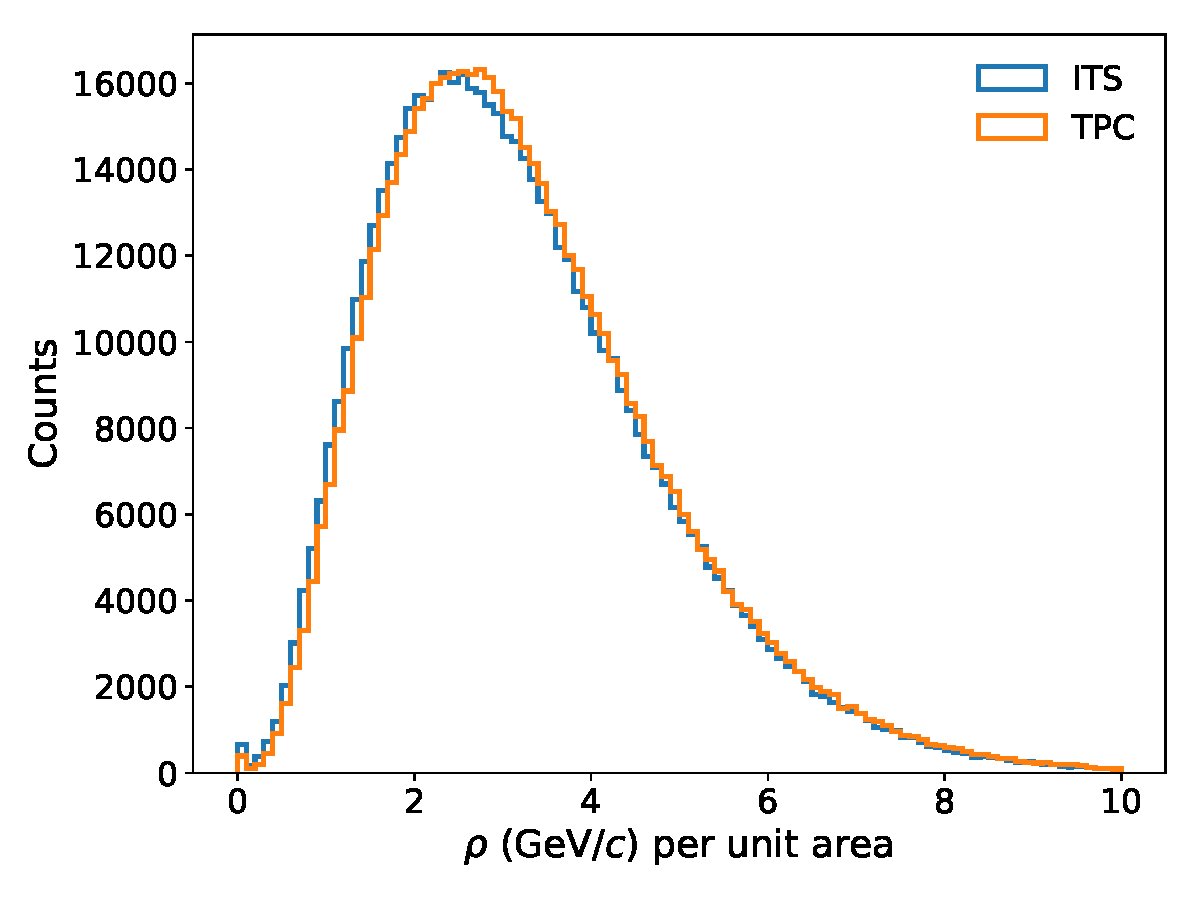
\includegraphics[width=0.49\textwidth]{Appendices/UEestimate_Skimmed_13def.pdf}
		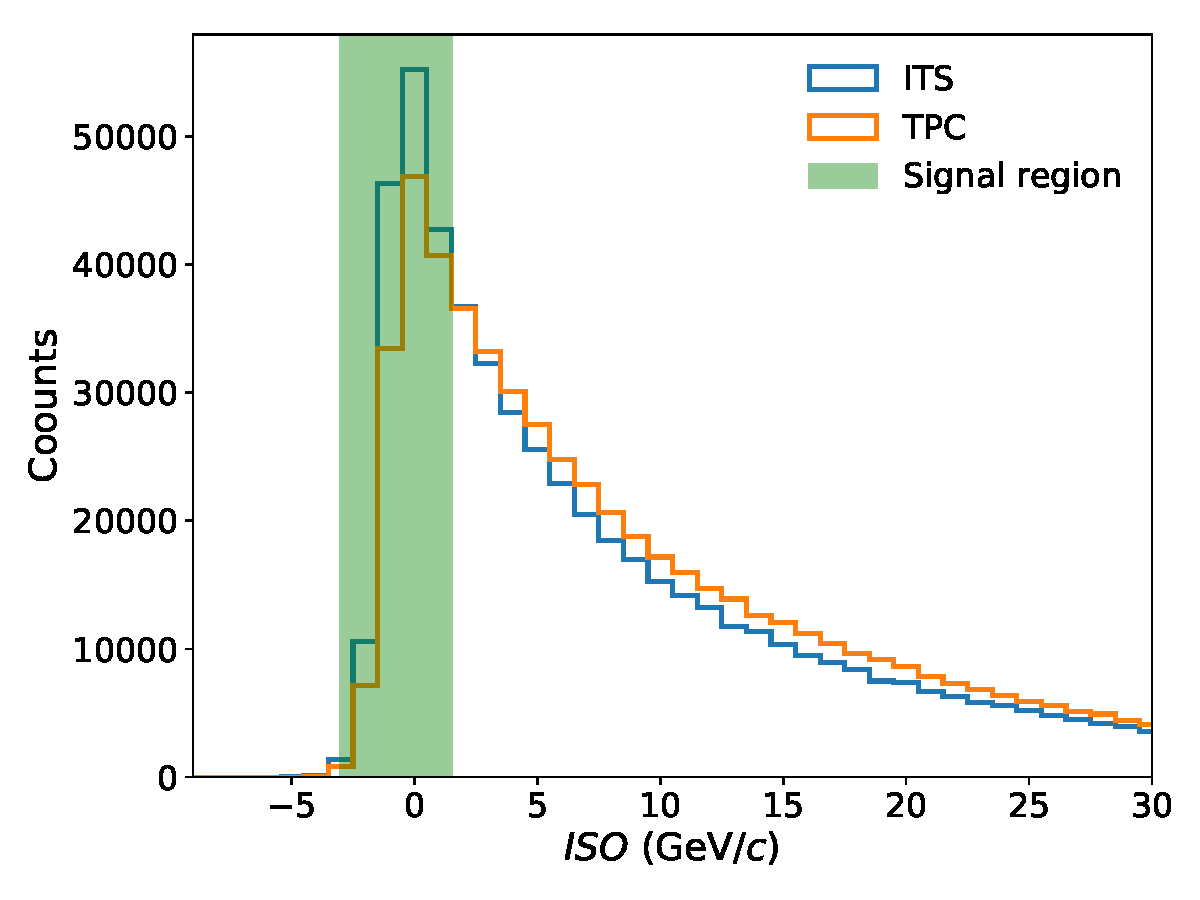
\includegraphics[width=0.49\textwidth]{Appendices/IsolationTPC_Skimmed_13def.pdf}
	\caption{Transverse momentum density (left panel) and isolation distributions (right panel) determined with ITS tracks (in blue) and TPC+ITS tracks (in orange) in \pPb~data.}
	\label{fig:pPb_its_tpc_rho}
\end{figure}

For simplicity we use the same threshold of 1.5 \GeVc~for our $\gammaiso$~candidates for both ITS-only and ITS+TPC tracks. We found that the isolation with ITS+TPC tracks leads to a better rejection of the background, which leads to an increased photon purity. This is shown in Figure~\ref{fig:ComparisonTPCITSiso_purity}. 

\begin{figure}
	\center
	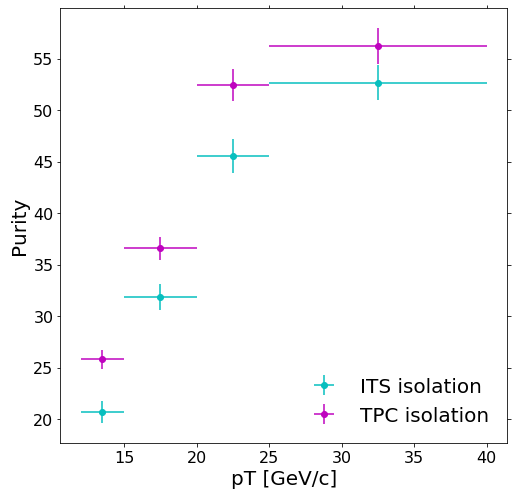
\includegraphics[width=0.49\textwidth]{Appendices/PurityITSTPC.png}
	\caption{Comparison of purity obtained in \pPb~collisions with isolation variable obtained with ITS-only tracks (purple) and with ITS+TPC tracks (cyan). The error bars represent statistical uncertainty only. }
	\label{fig:ComparisonTPCITSiso_purity}
\end{figure}

We checked our main results (correlation function) in \pPb~data by performing our analysis with isolation variable, UE estimate, and corresponding purity values separately for ITS-only tracks and ITS+TPC tracks. As shown in Figure~\ref{fig:ComparisonTPCITSiso_frag}, we obtain consistent results. We obtain a slightly better statistical uncertainty when including TPC (a relative uncertainty of 22$\%$ to 41$\%$ depending on \zt~vs 24$\%$ to $51\%$ for the ITS case), which an be attributed to the corresponding higher purity. However, these slightly better statistical uncertainties do not change the main result of our paper. For consistency with pp results (where we cannot use ITS+TPC tracks because the TPC was not read out), we chose to report our results for ITS-only tracks. 

\begin{figure}
	\center
	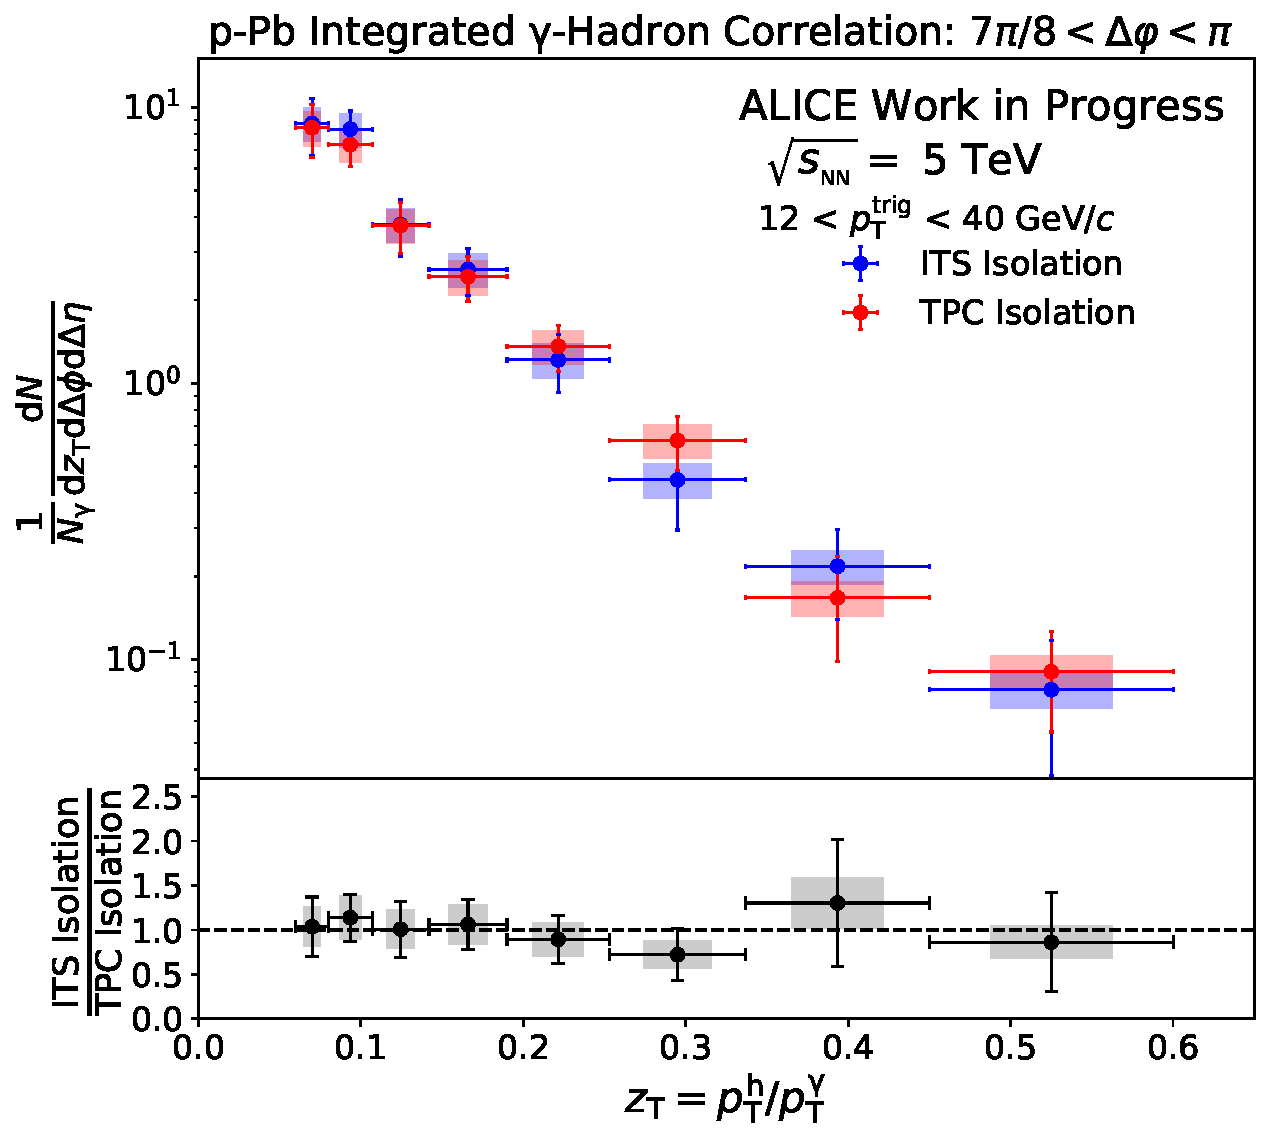
\includegraphics[width=0.49\textwidth]{Appendices/ISO_Compare_Final_FFunction_and_Ratio}
	\caption{Comparison of fragmentation function measurement in \pPb~collisions with isolation variable obtained with ITS-only tracks (blue) and with ITS+TPC tracks (red).}
	\label{fig:ComparisonTPCITSiso_frag}
\end{figure}

We consider this study comparing ITS-only tracking and ITS+TPC tracks as a check against possible biases due to worse momentum resolution or fake rate of the ITS-only tracking. Given that we have obtained consistent results with the standard ITS+TPC tracking, we do not assign an additional systematic uncertainty for the tracking performance on UE-estimate and isolation variables. 

%\FloatBarrier
\section{Comparison to ABCD method results}
\label{sec:comparisontoABCD}
In this section we compare our results obtained with the template fit method to the ABCD method results obtained by Erwann Masson for his isolated-photon analysis in \pPb~data~\cite{Erwann}. That study is performed with the same \pPb~data using the same event and cluster selections and a similar isolation criterion that uses only charged-particles (shown in the Appendix of Ref.~\cite{Erwann}).

Figure~\ref{fig:ComparisonToErwanns} shows our results compared to the results of the ABCD method. We show both our results using ITS-only tracks and ITS-TPC tracks (which is more directly comparable to the ABCD result). Our results are systematically below the ABCD method, but they are consistent within 1$\sigma$ systematic uncertainty for most of the $\pt$ range. 
%Given that the two methods are independent, and the systematic uncertainties are estimated independently, this level of agreement in principle constrains the systematic uncertainties, although a full evaluation of the correlation of the systematic uncertainties of the two methods is outside the scope of this analysis. 

%Previous analyses of isolated photons have used the ``matrix'' or ``ABCD'' method with an isolation variable that considers both charged particles and calorimeter clusters. The issue of bias due to the ``factorization'' assumption, i.e the correlation between the isolation variable and the shower-shape variable, has been studied in great detail\footnote{See for example D. Lodato's thesis, CERN-THESIS-2017-307.}. It has been shown that the ``non-factorization" bias comes from neutral energy in the isolation because that introduces a correlation through meson decays. The use of an isolation variable that only considers charged-particles limits the biases, corrections and associated systematic uncertainties, at the expense of a slightly lower purity. 

\begin{figure}[h]
\center
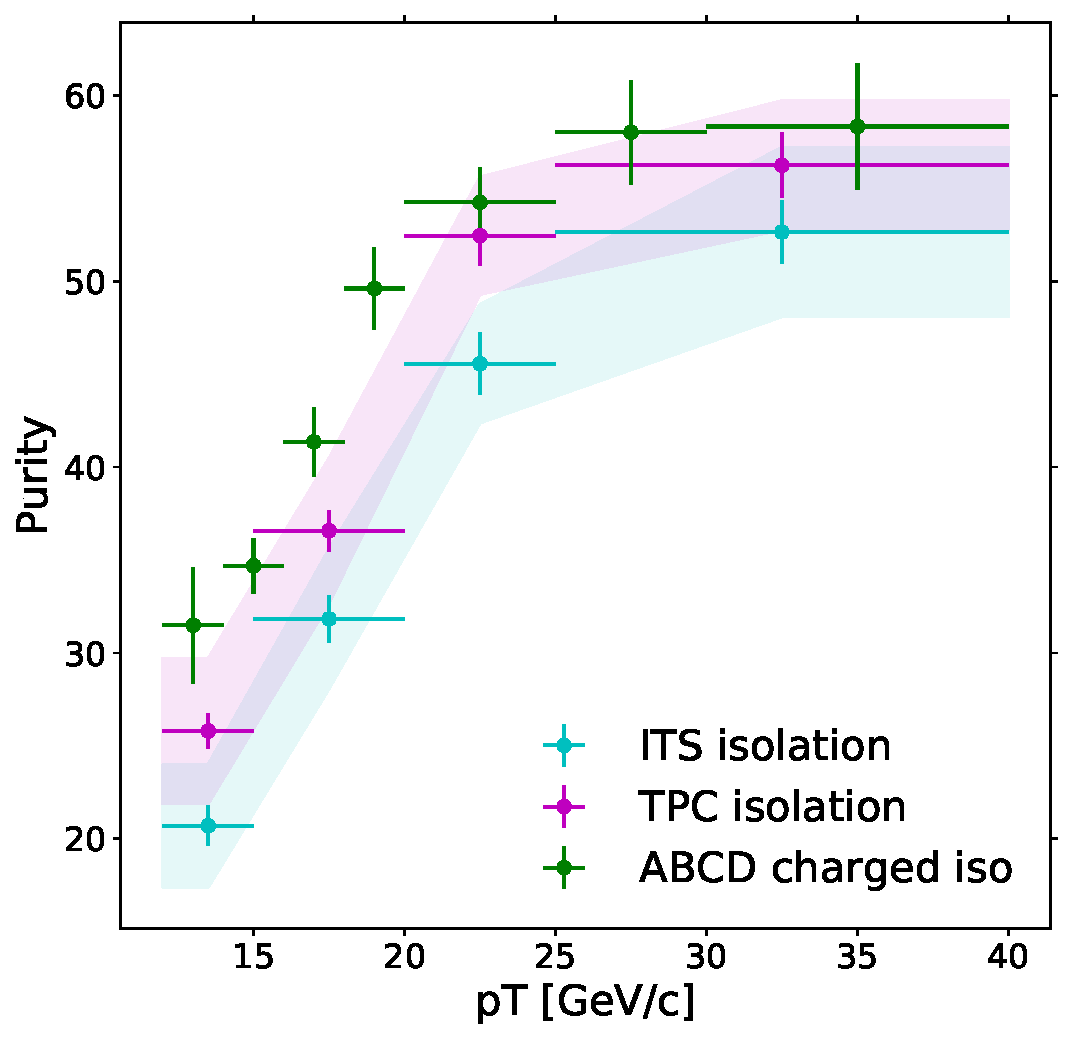
\includegraphics[width=0.5\textwidth]{Appendices/ABCDcomparison.pdf}
\caption{Comparison between purity measured with the template fit and ABCD method, from Ref.~\cite{Erwann}, in \pPb~data. The error bars represent statistical uncertainty only and the bands represent the systematic uncertainty only.}
\label{fig:ComparisonToErwanns}
\end{figure}



\section{Check by splitting clusters in $|\eta|<0.4$ and $0.4<|\eta|<0.67$ }

In our analysis, we use clusters with $|\eta|<0.67$ (Section~\ref{sec:clusterselection}); we consider an isolation variable constructed with tracks with $|\eta|<0.8$ (Section~\ref{sec:tracking}) and a cone size of $R=$0.4 (Section~\ref{sec:isolation}). The isolation cone is thus fully contained in the tracking acceptance only for clusters with $|\eta|<0.4$; the isolation cone for clusters with $0.4<|\eta|<0.67$ is only partially covered in pseudorapidity angle. 
Note that the tracking acceptance covers the full azimuthal angle so this is not an issue in azimuth. 

To check for possible biases that this partial containment of isolation cone in pseudorapidity we did split all the measured clusters into two categories: $|\eta|<0.4$ and $0.4<|\eta|<0.67$. In principle, if the bias introduced by the lack of total coverage of the isolation cone would lead to higher background in the $0.4<|\eta|<0.67$ region (background might appear less-isolated than in reality, and might pass the selection), and thus lead to a lower purity. We perform this study in the \pPb~data, which has better statistical precision than the pp data and would allow us to better constrain small biases. The comparison of purity measurements is shown in Figure~\ref{fig:spliteta}. Both set of measurements are compatible within statistical uncertainties. Thus, we conclude that the potential bias due to incomplete coverage of isolation cone is negligible and we do not assign any systematic uncertainty to this source. We explain this observation by noting that the azimuthal angle is fully covered, and that most of the energy in the isolation cone is within small angles of the neutral-mesons that 
%bvj represents 
dominate the background (the background is primarily high-z neutral mesons in jets). 

\begin{figure}
	\center
	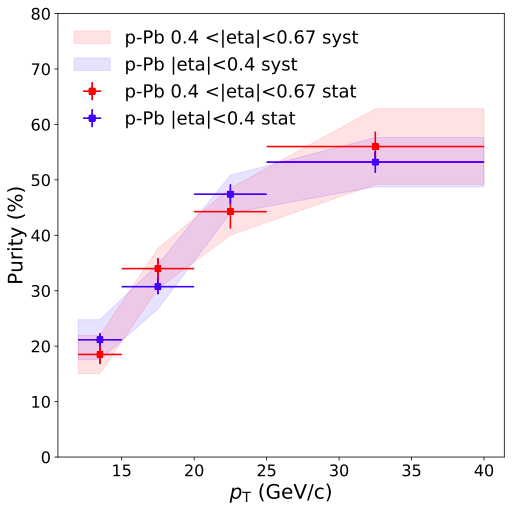
\includegraphics[width=0.5\textwidth]{SplitEtaStudy.png}
	\caption{Purity measurement in \pPb~collisions for clusters with $|\eta|<0.4$ and $0.4<|\eta|<0.67$.}
	\label{fig:spliteta}
\end{figure}

\section{Cluster selection variations}
\label{sec:clustercutselectionvariation}
In this section, we study the impact on our purity measurement of variations in our cluster selection (Section~\ref{sec:clusterselection}). It should be noted that the purity by itself is not a physical quantity. It is entirely cut-dependant, where a higher purity often results in a lower efficiency. As a result, the variations in this analysis are not used to estimate an uncertainty on the purity.

First, we study the impact of our number-of-local maximum criteria for clusters. The NLM $<3$ selection was used in previous isolated photon analyzes (e.g. Ref~\cite{Acharya:2019jkx,Erwann}), where it was found to help to improve the simulation description of the background shower-shape. Figure~\ref{fig:numberoflocalmaxima} shows the purity measurement with and without this selection in pp and \pPb~data. We observe no significant difference.

\begin{figure}
	\center
	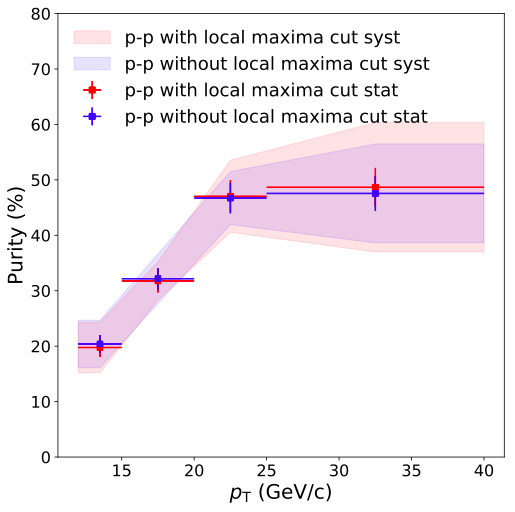
\includegraphics[width=0.495\textwidth]{G-H_New/dPhi_to_0/NLMvariation_pp.png}
	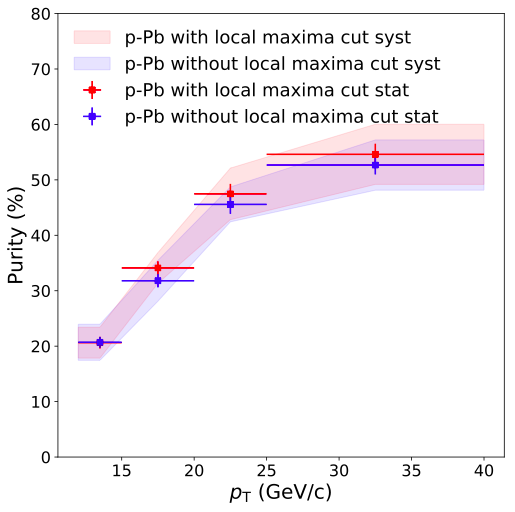
\includegraphics[width=0.495\textwidth]{NLMvariation_pPb.png}
	\caption{Purity measurement with and without cluster selection based on number-of-local maxima in pp (left) and \pPb~(right) collisions.}
	\label{fig:numberoflocalmaxima}
\end{figure}

In Figure~\ref{fig:distancetobadchannel} we show our purity measurement by varying the distance-to-bad channel cut from our nominal $\geq 1$ to $\geq 2$. This change would remove about 20$\%$ of our \gammaiso~candidates. We observe no significant difference. 

\begin{figure}
	\center
	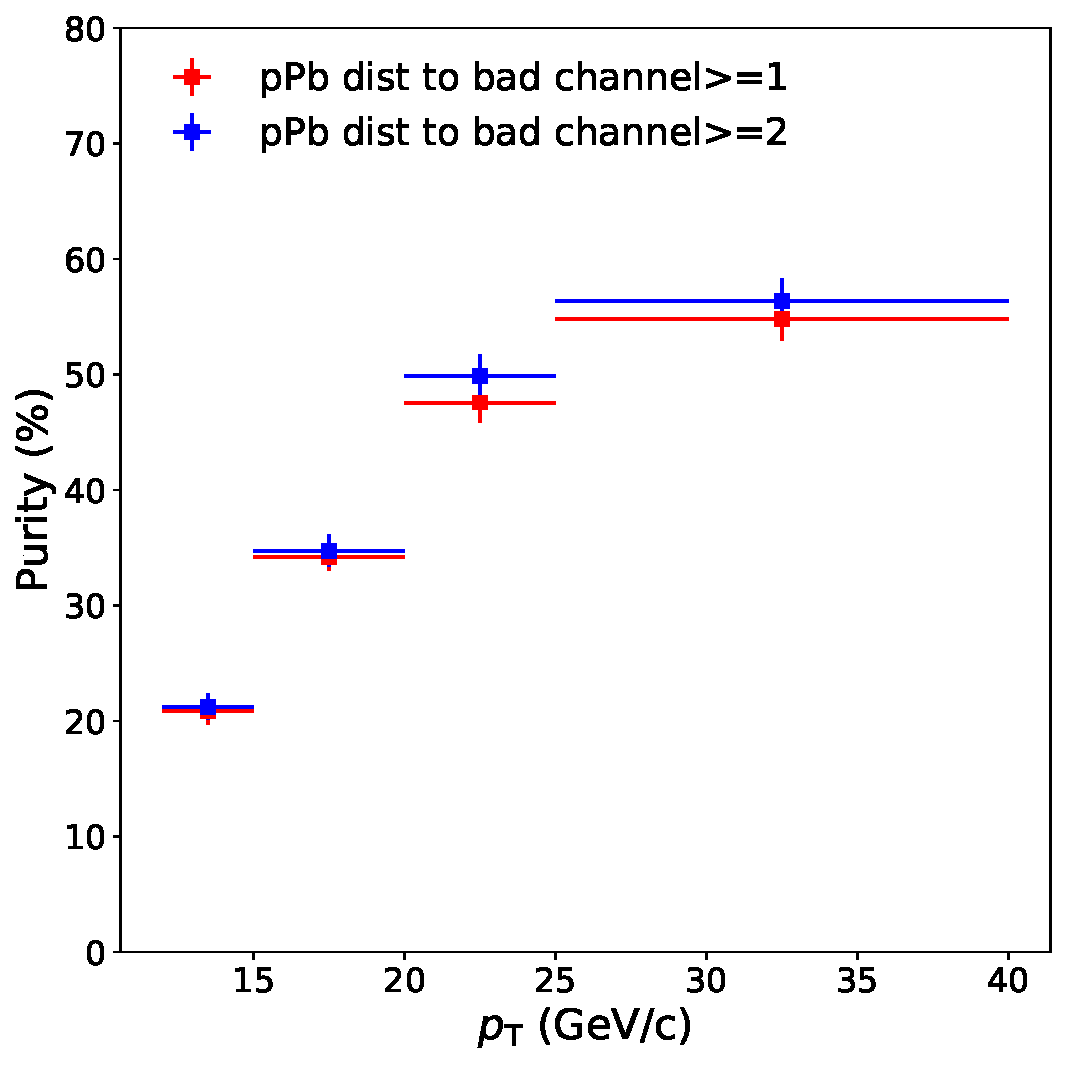
\includegraphics[width=0.495\textwidth]{Appendices/ppbdistance.pdf}
	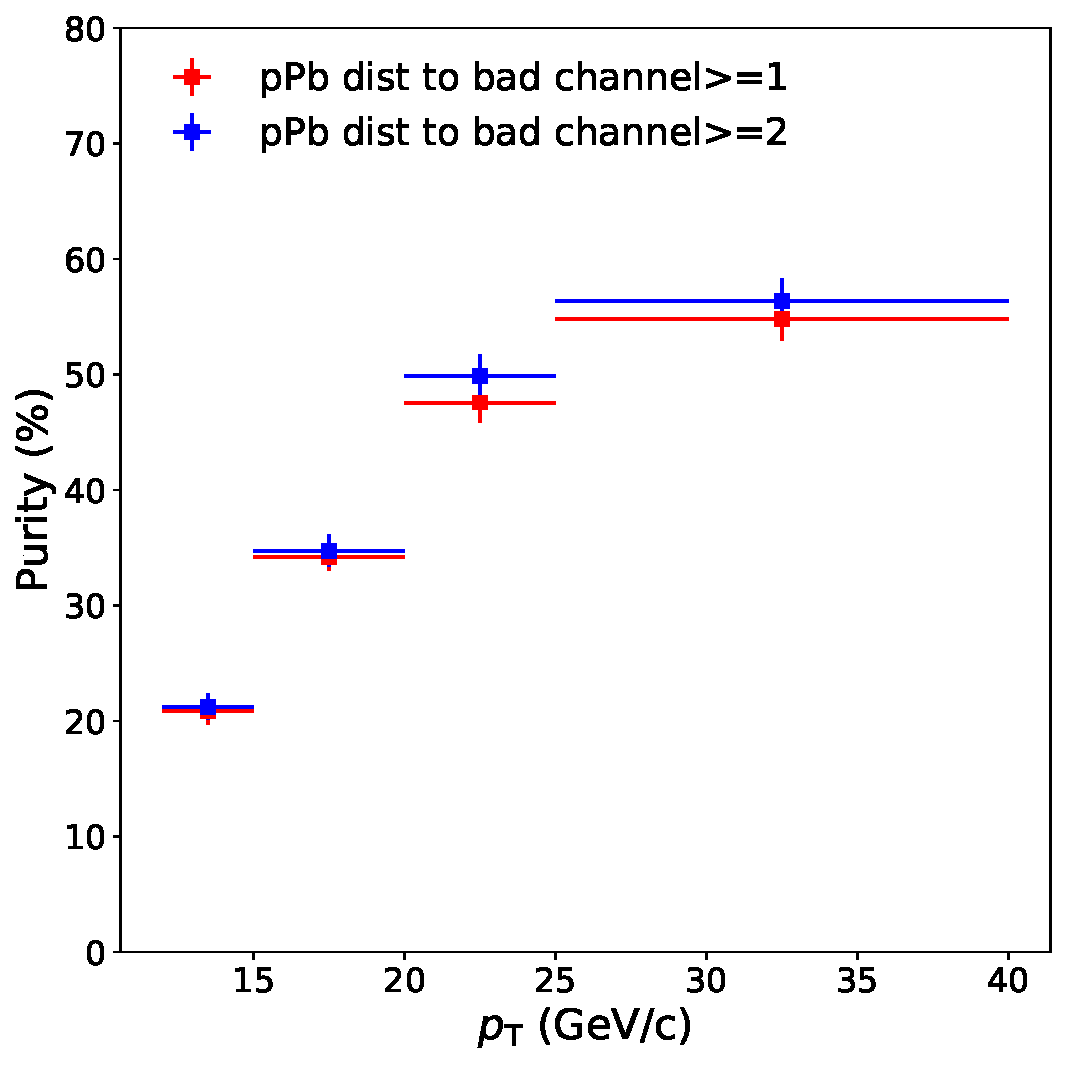
\includegraphics[width=0.495\textwidth]{Appendices/ppbdistance.pdf}
	\caption{Purity measurement with distance-to-bad channel $\geq 1$ (nominal) and $\geq 2$ in pp (left) and \pPb~(right) data.}
	\label{fig:distancetobadchannel}
\end{figure}

In Figure~\ref{fig:TOF} we show our purity measurement with and without cluster time selection. We observe no significant difference. 

\begin{figure}
	\center
	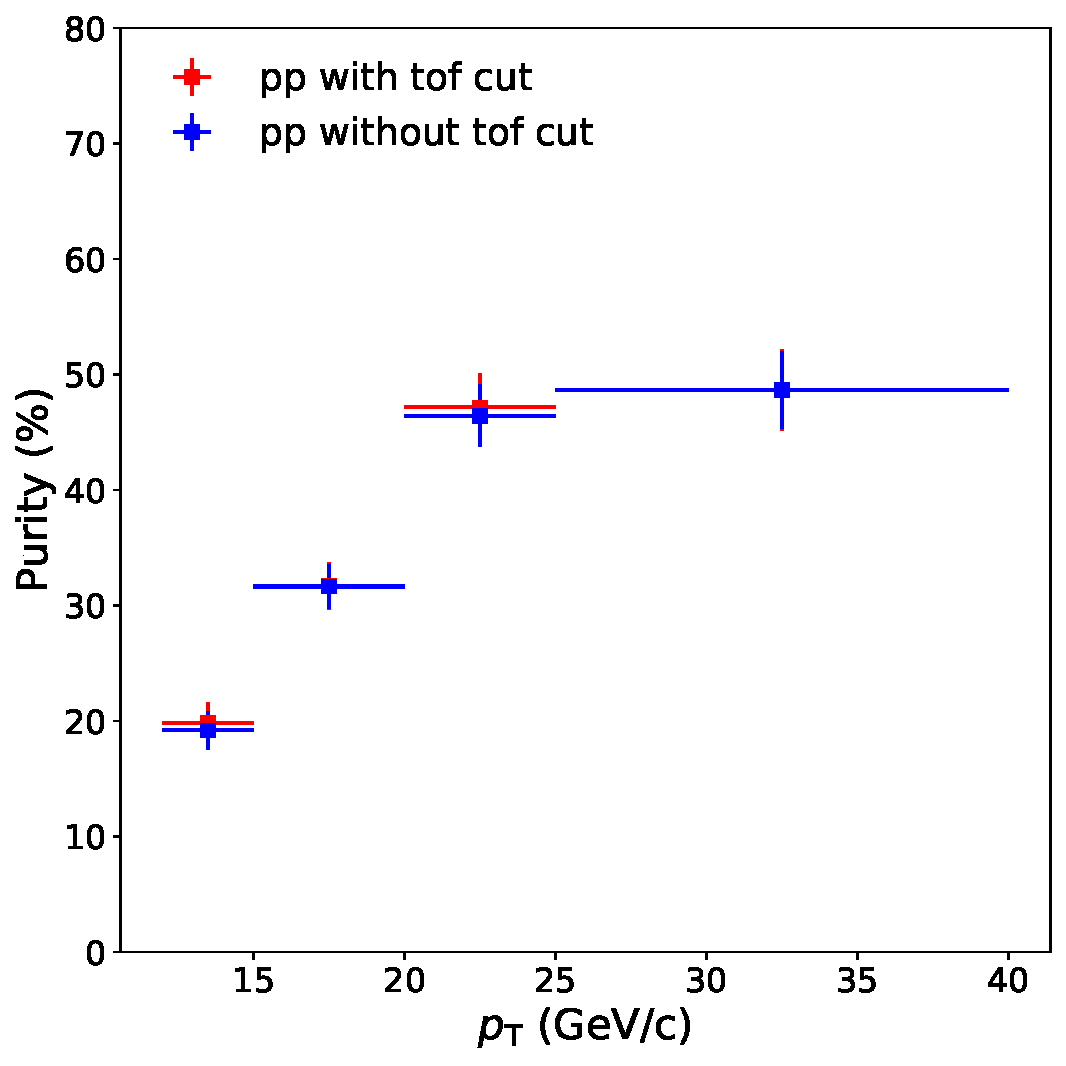
\includegraphics[width=0.495\textwidth]{Appendices/pptof.pdf}
	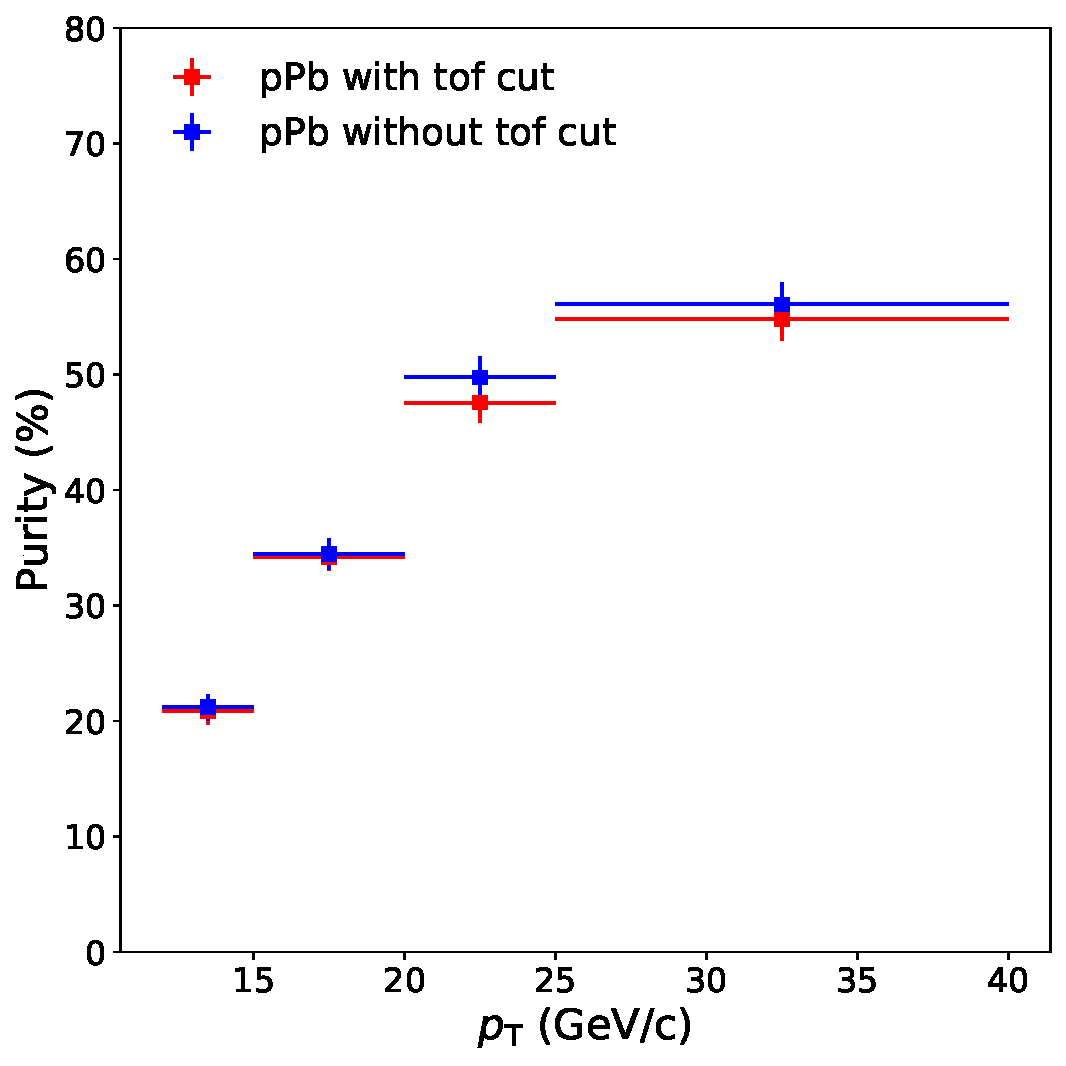
\includegraphics[width=0.495\textwidth]{Appendices/ppbtof.pdf}
	\caption{Purity measurement with and without time cut $(\Delta t<20$ ns) in pp (left) and \pPb~(right) data.}
	\label{fig:TOF}
\end{figure}

In Figure~\ref{fig:exoticity} we show our purity measurement with an exoticity cut with a threshold of 5\% (nominal) and a variation of $3\%$. We observe no significant difference. 

\begin{figure}
	\center
	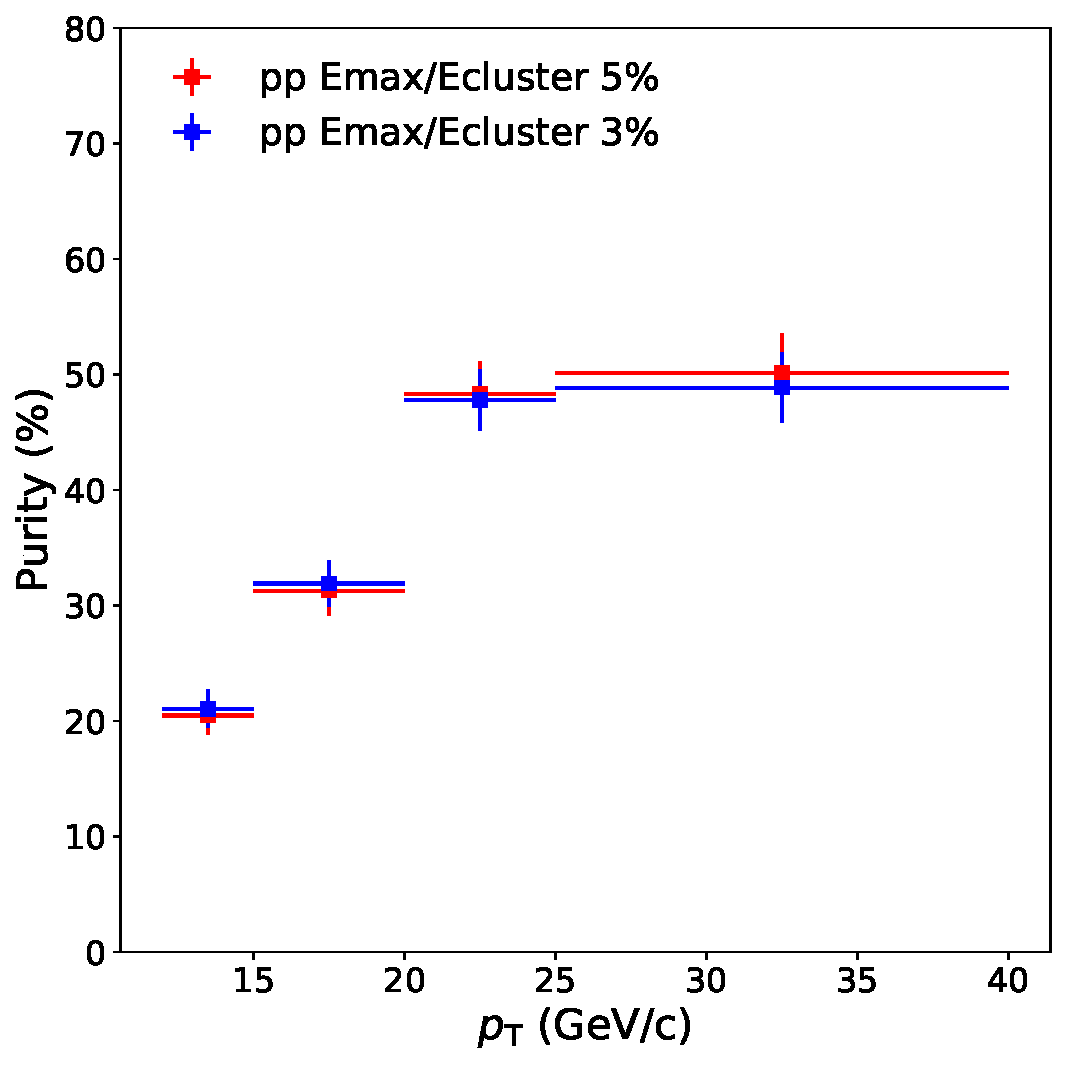
\includegraphics[width=0.495\textwidth]{Appendices/ppemax.pdf}
	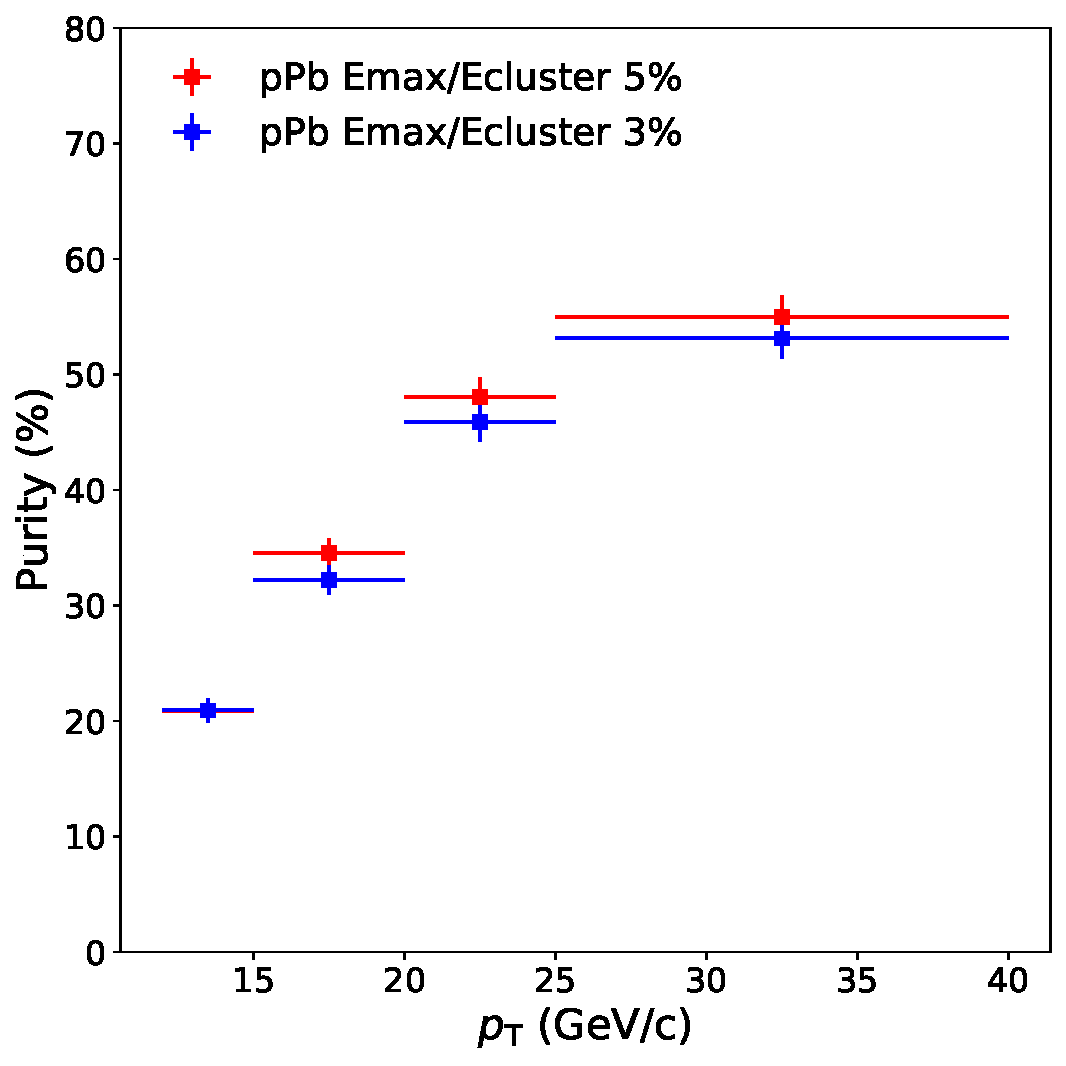
\includegraphics[width=0.495\textwidth]{Appendices/ppbemax.pdf}
	\caption{Purity measurement with an exoticity cut of 5$\%$ (nominal) and 3$\%$ in pp (left) and \pPb~(right) data.}
	\label{fig:exoticity}
\end{figure}

In Figure~\ref{fig:isolationvariation} we show our purity measurement with different isolation thresholds. We vary our nominal threshold of 1.5 $\GeVc$ by $\pm$ 0.2 \GeVc. As expected the higher (lower) isolation threshold results in a lower (higher) purity. However, the difference with respect to our nominal result is small with respect to our statistical and systematic uncertainties. This indicates that the purity measurement has only a weak dependence on the choice of isolation threshold. 



\begin{figure}
	\center
	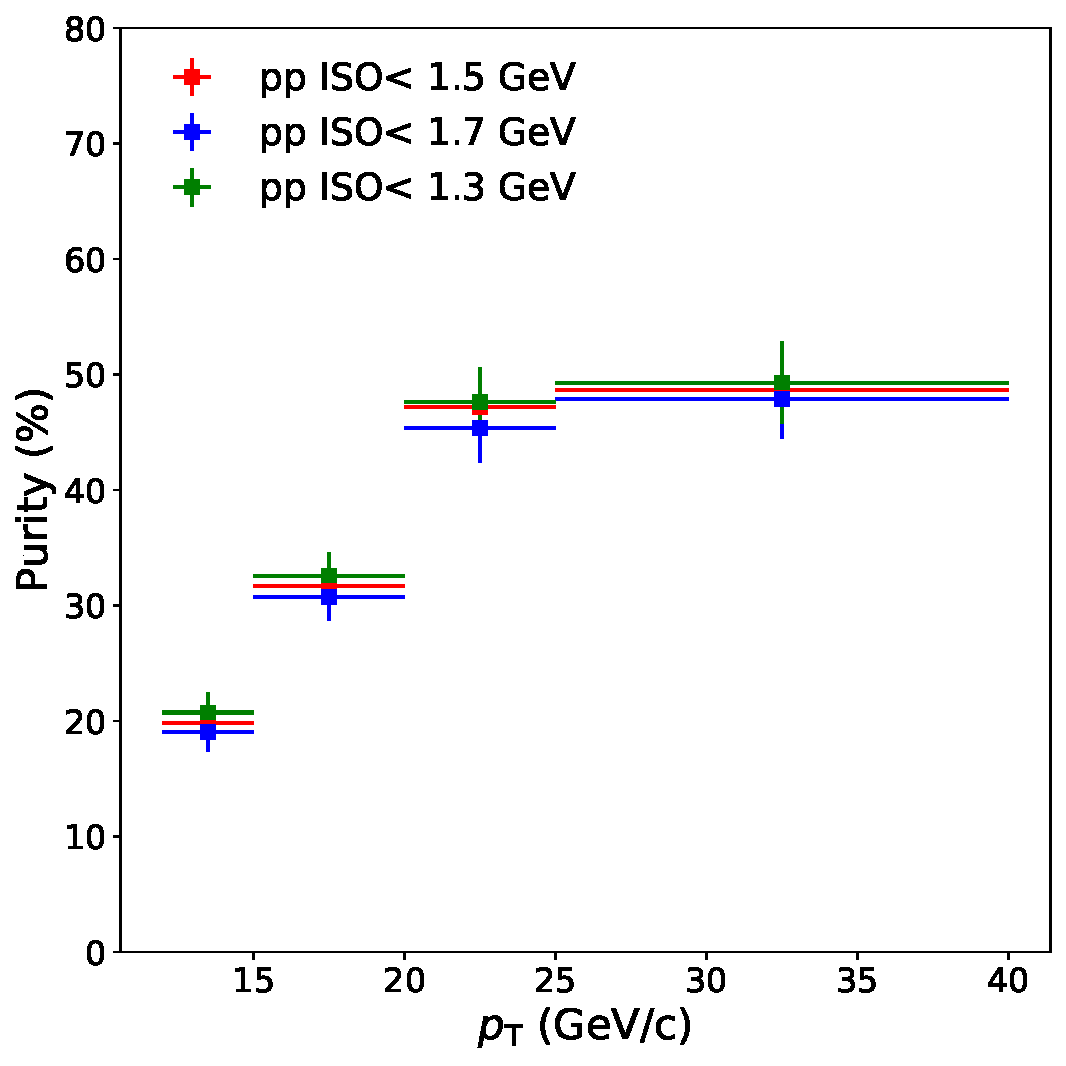
\includegraphics[width=0.495\textwidth]{Appendices/ppiso.pdf}
	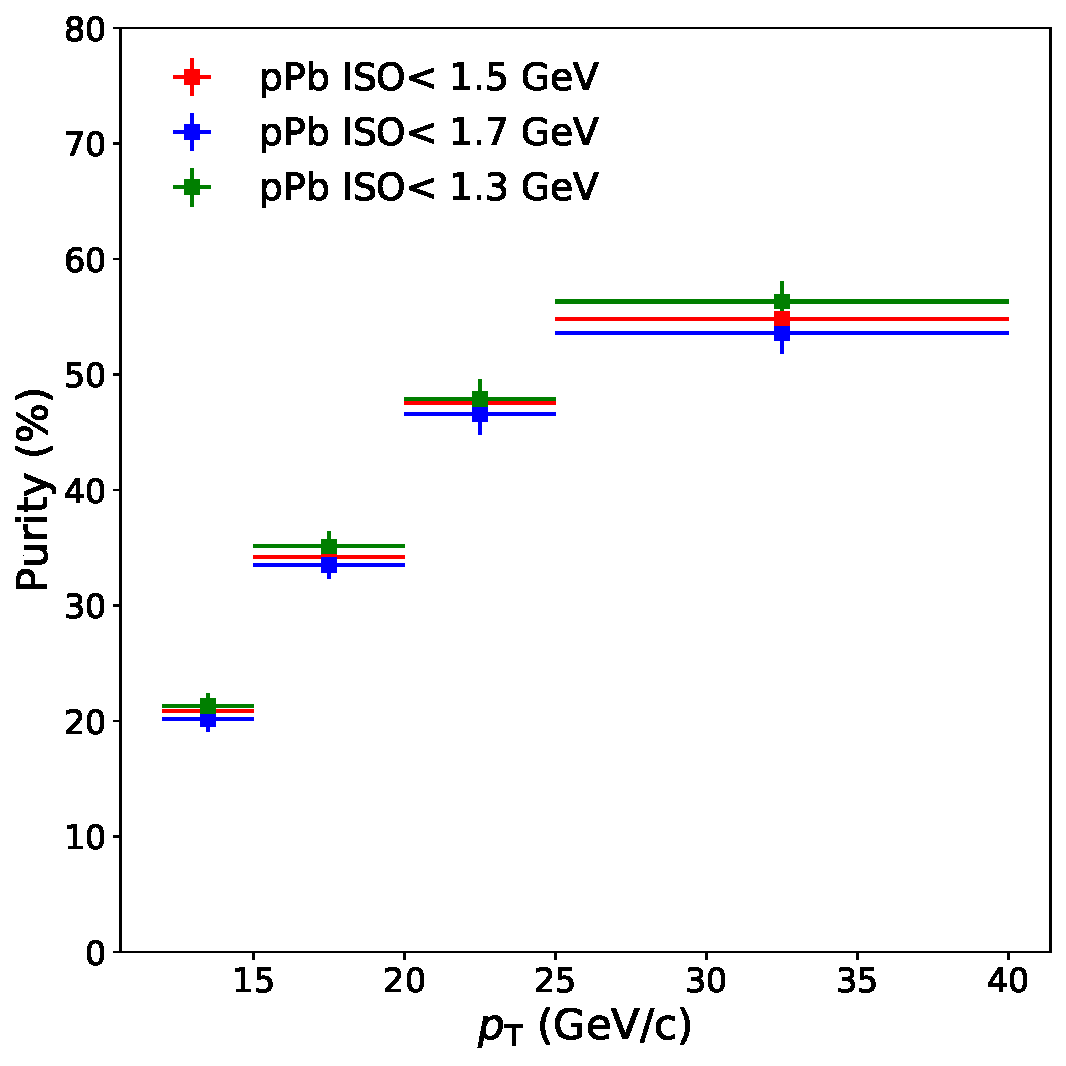
\includegraphics[width=0.495\textwidth]{Appendices/ppbiso.pdf}
	\caption{Purity measurement with different isolation threshold requirements in pp (left) and \pPb~(right) data.}
	\label{fig:isolationvariation}
\end{figure}




Given that the impact of these cluster variations on our purity measurement is small compared to our estimated systematic uncertainties (described in Section~\ref{sec:puritysystematics}), we do not assign an additional systematic uncertainty due to cluster selection. 

\section{MC-based correction for background template}
\label{sec:MCbasedcorrection}

Figure~\ref{fig:bkgCorrection} shows the weight correction (see Equation~\ref{eq:bkgtemplatecorrection}) applied to the anti-isolation shower-shape distribution, which is obtained from dijet MC simulation. As described in more detail in Section~\ref{sec:purity}, only the shape of this correction is relevant as the normalization is actually fixed in the template fit. The systematic uncertainty associated with this correction is obtained with a double-ratio using data in the background-dominated region ($\lambdasquare>0.4$), as described in more detail in Section~\ref{sec:puritysystematics}. 

\begin{figure}
	\center
	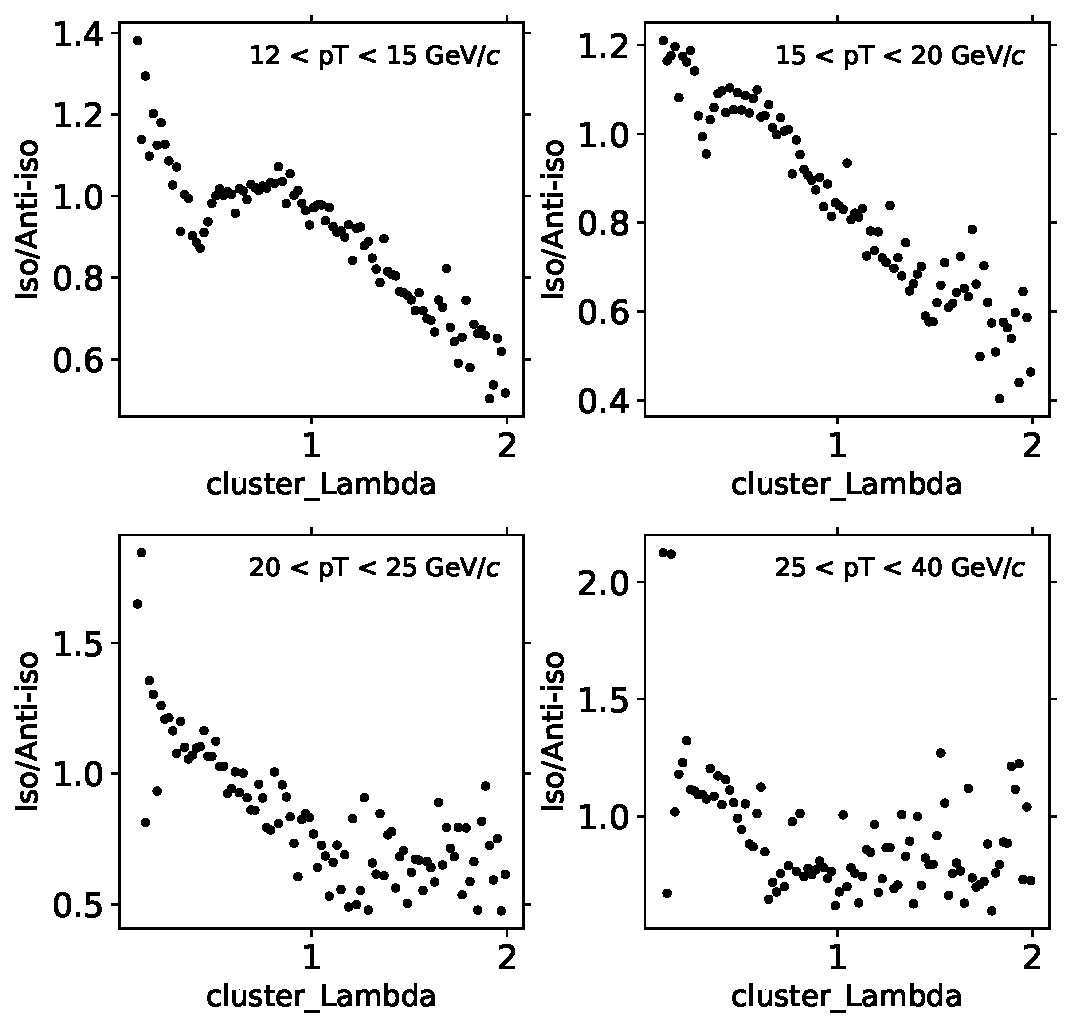
\includegraphics[width=0.76\textwidth]{Appendices/bkg-template-correction-p-Pb}
	%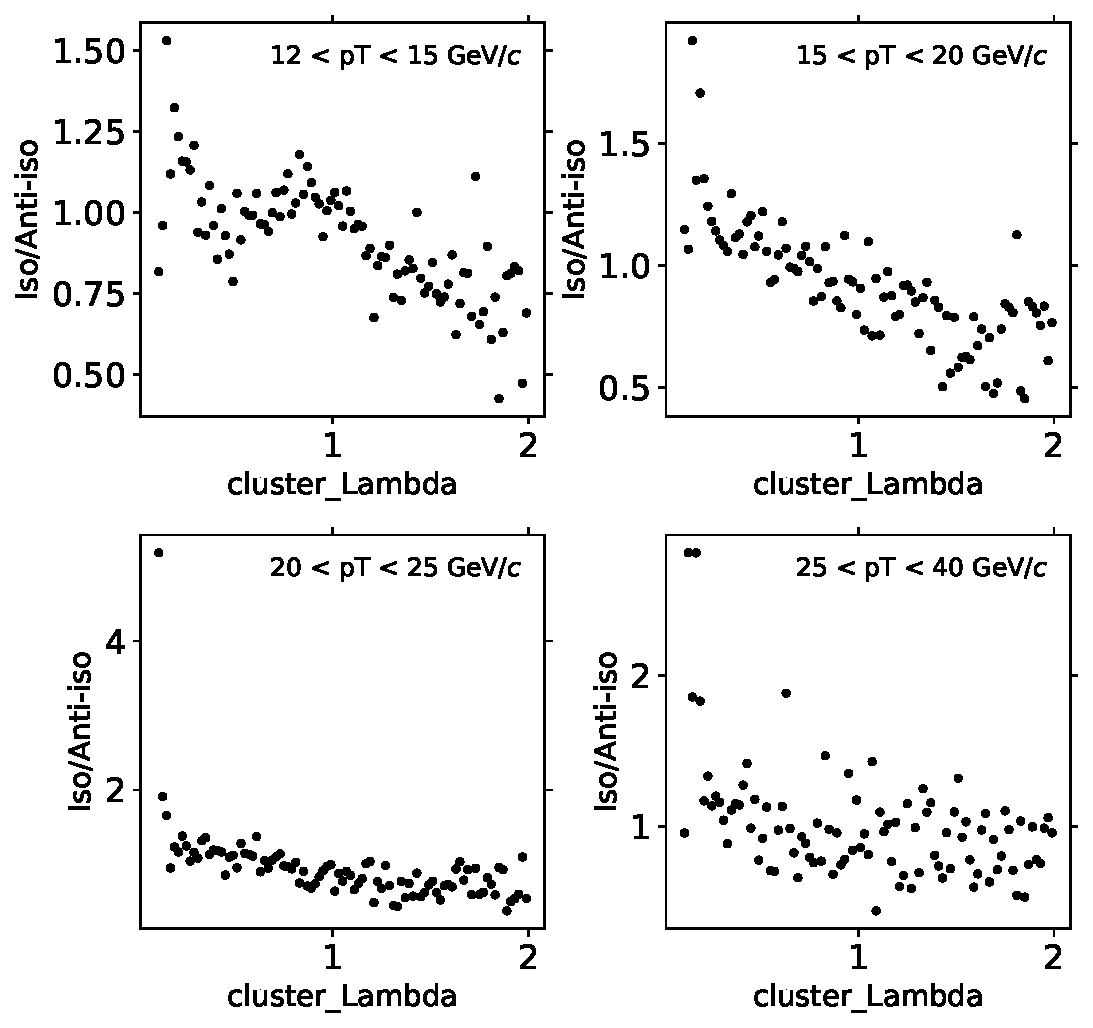
\includegraphics[width=0.495\textwidth]{Appendices/bkg-template-correction-pp}
	\caption{MC-based correction applied to the background shower-shape template for \pPb~collisions in various $\pt$ ranges.}
	\label{fig:bkgCorrection}
\end{figure}

\section{Smearing signal template}
\label{sec:smearingsignaltemplate}
As part of our investigations to evaluate the template fit systematic uncertainty, we performed studies ``smearing" of the signal-shape template. That is, for each cluster we smear the measured \lambdasquare~by multiplying it by some random number drawn from a Gaussian centered at unity with a given standard deviation ``smearing width".

\begin{figure}
	\center
	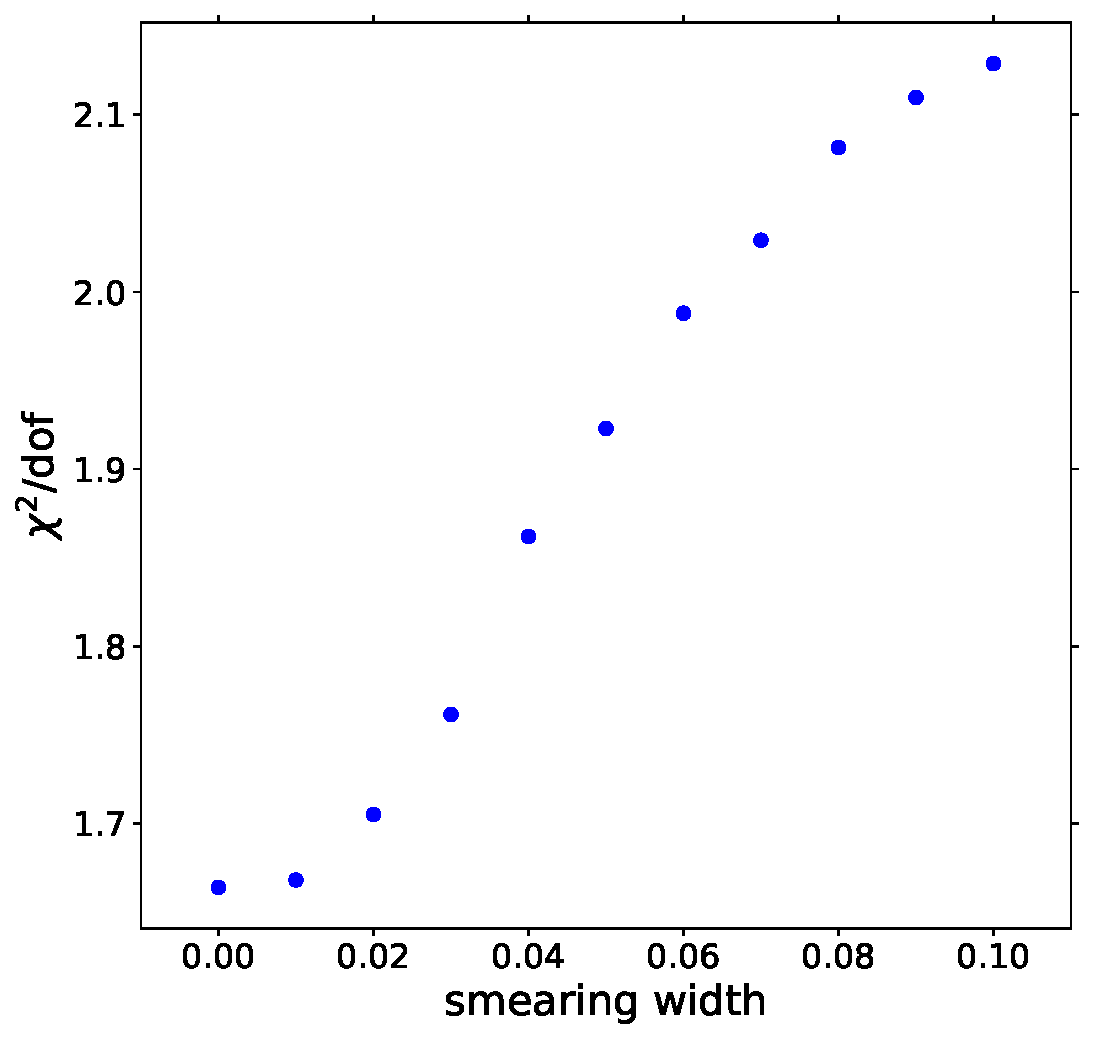
\includegraphics[width=0.495\textwidth]{Appendices/smeared-chi2s-pp-cluster_Lambda-15-20.pdf}
		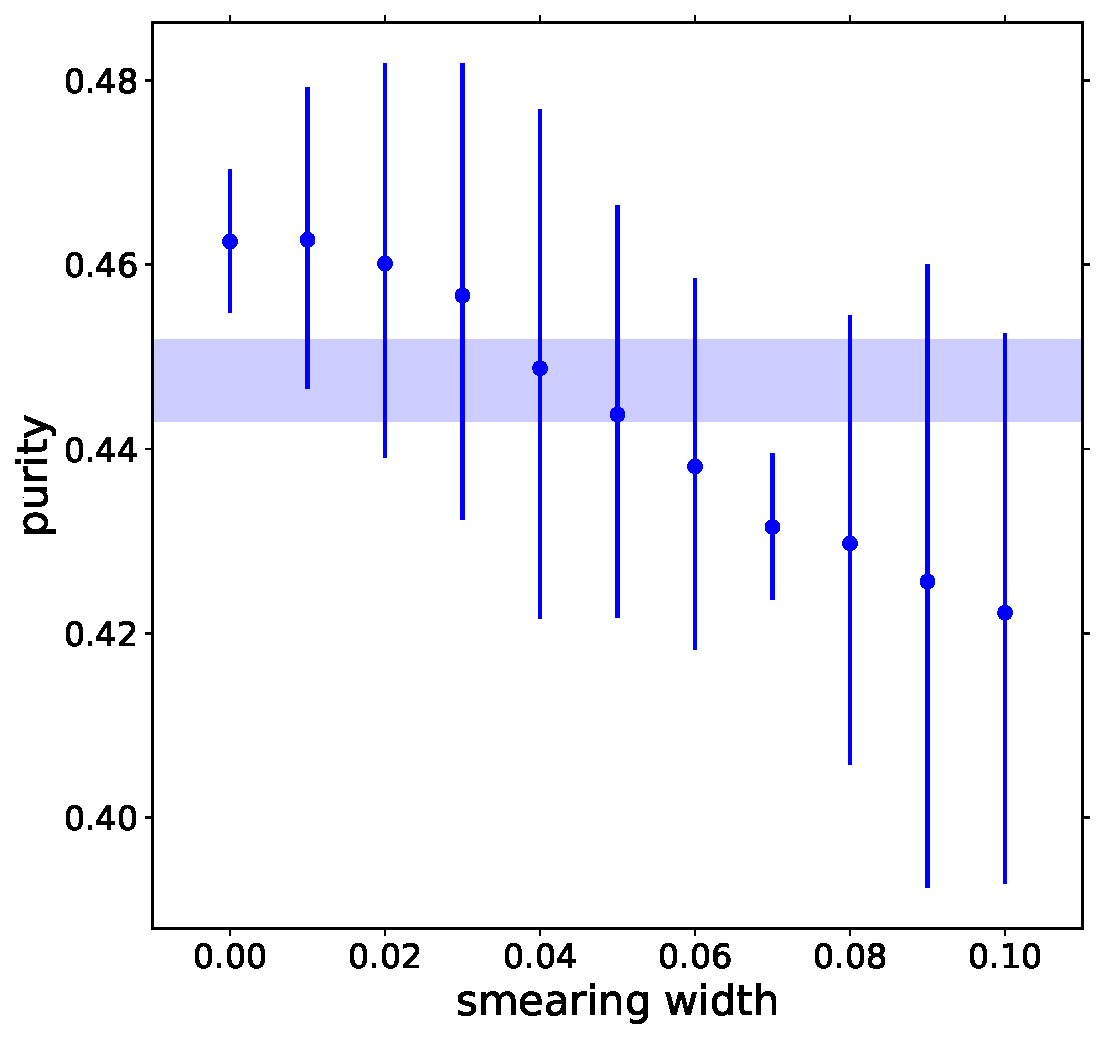
\includegraphics[width=0.495\textwidth]{Appendices/smeared-purities-pp-cluster_Lambda-15-20.pdf}
		\caption{Left: Signal template distribution for various smearing widths. Right: purity vs smearing width. The error bar represents the statistical uncertainty, which has been scaled by $\sqrt{\chi^{2}/\mathrm{DOF}}$.}
	\label{fig:smearingSignalShape}
\end{figure}

Figure~\ref{fig:smearingSignalShape} shows the purity obtained for $15<\pt<20$ \GeVc~as a function of smearing width used and the corresponding $\chi^{2}$/DOF. We observe rather significant deterioration of the $\chi^{2}$ with increasing smearing width, which indicates that smearing beyond $\approx3\%$ are strongly disfavoured by the data. To account for the deterioration of the $\chi^{2}$ that we observe with the smearing, we multiply the statistical error of the purity by a scaling factor of $\sqrt{\chi^{2}/\mathrm{DOF}}$. We find a trend of decreasing purity with increasing smearing width but this the trend is ``not significant", i.e. it can be accounted by the artificial worsening of the goodness-of-fit. 


We fit a constant to the purity values vs smearing widths (shown as band in Figure~\ref{fig:smearingSignalShape}). The error on that constant fit and its deviation of its central value from the nominal result (smearing width equal to zero) is below and absolute 1$\%$ difference, which is much smaller than our signal-template uncertainty based on the background-only template fit described in Section~\ref{sec:puritysystematics}. We reach the same conclusion for all \pt~ranges and for pp and \pPb~data.  


\section{Checking sensitivity to $\Delta\varphi$ binning }

Here we quantify the impact of our choice of binning in the correlation functions. The binning in principle could affect the ZYAM estimate and the shape of the correlation peak. We show results doubling the number of $\Delta\varphi$ bins. We do this for simplicity given that we want to be able to integrate the correlation in exactly the same window as reported in our nominal results ($\Delta\varphi>7\pi/8$). Figure~\ref{fig:dPhivariation} shows the correlation function obtained with double the number of bins as the nominal result. The main conclusion of our study does not change: in every \zt~bin, the pp and \pPb~data are compatible within uncertainties (as quantified in the figure by the $\chi^{2}$~and corresponding p-value), and the \textsc{Pythia8} describes the data within uncertainties. 

\begin{sidewaysfigure}
\label{fig:dPhivariation}
\centering
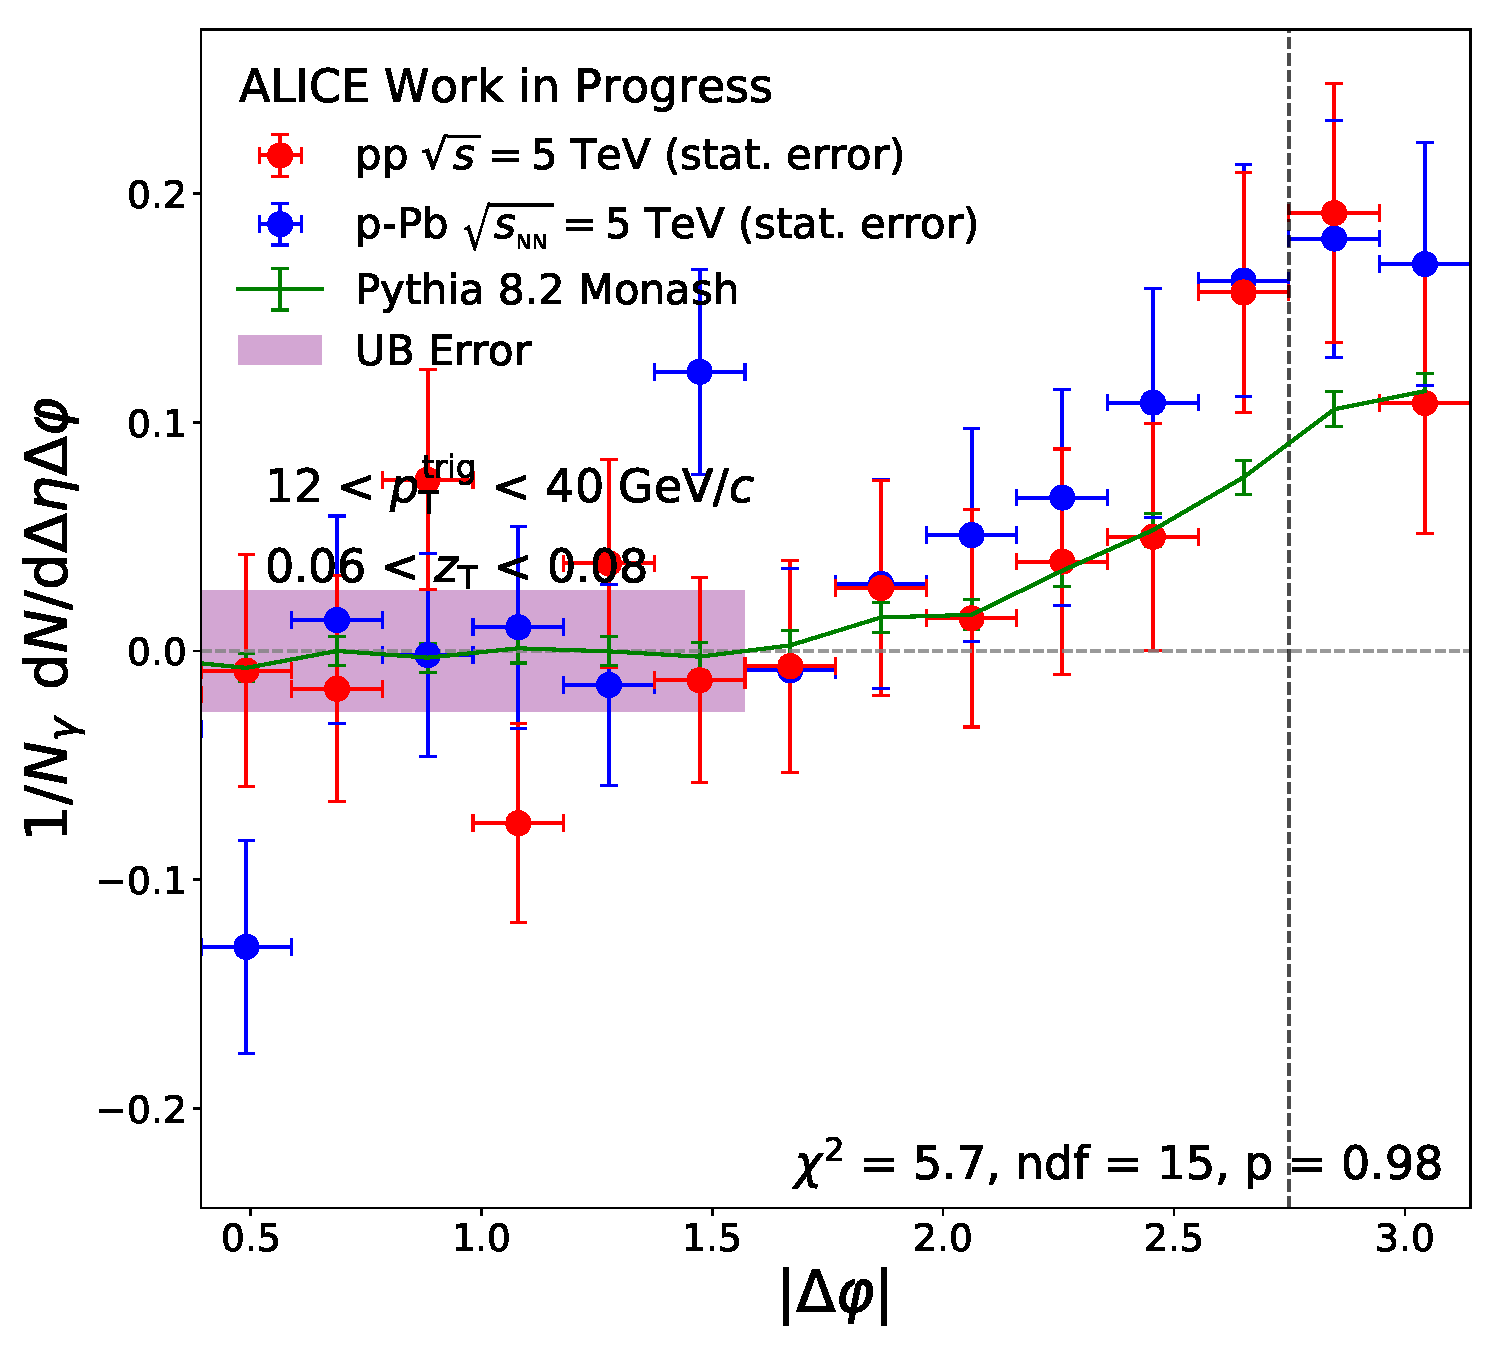
\includegraphics[width = 0.24 \textwidth]{G-H_New/16_dPhi/Cs_Final_Indv_pT_0_zT_0.pdf}
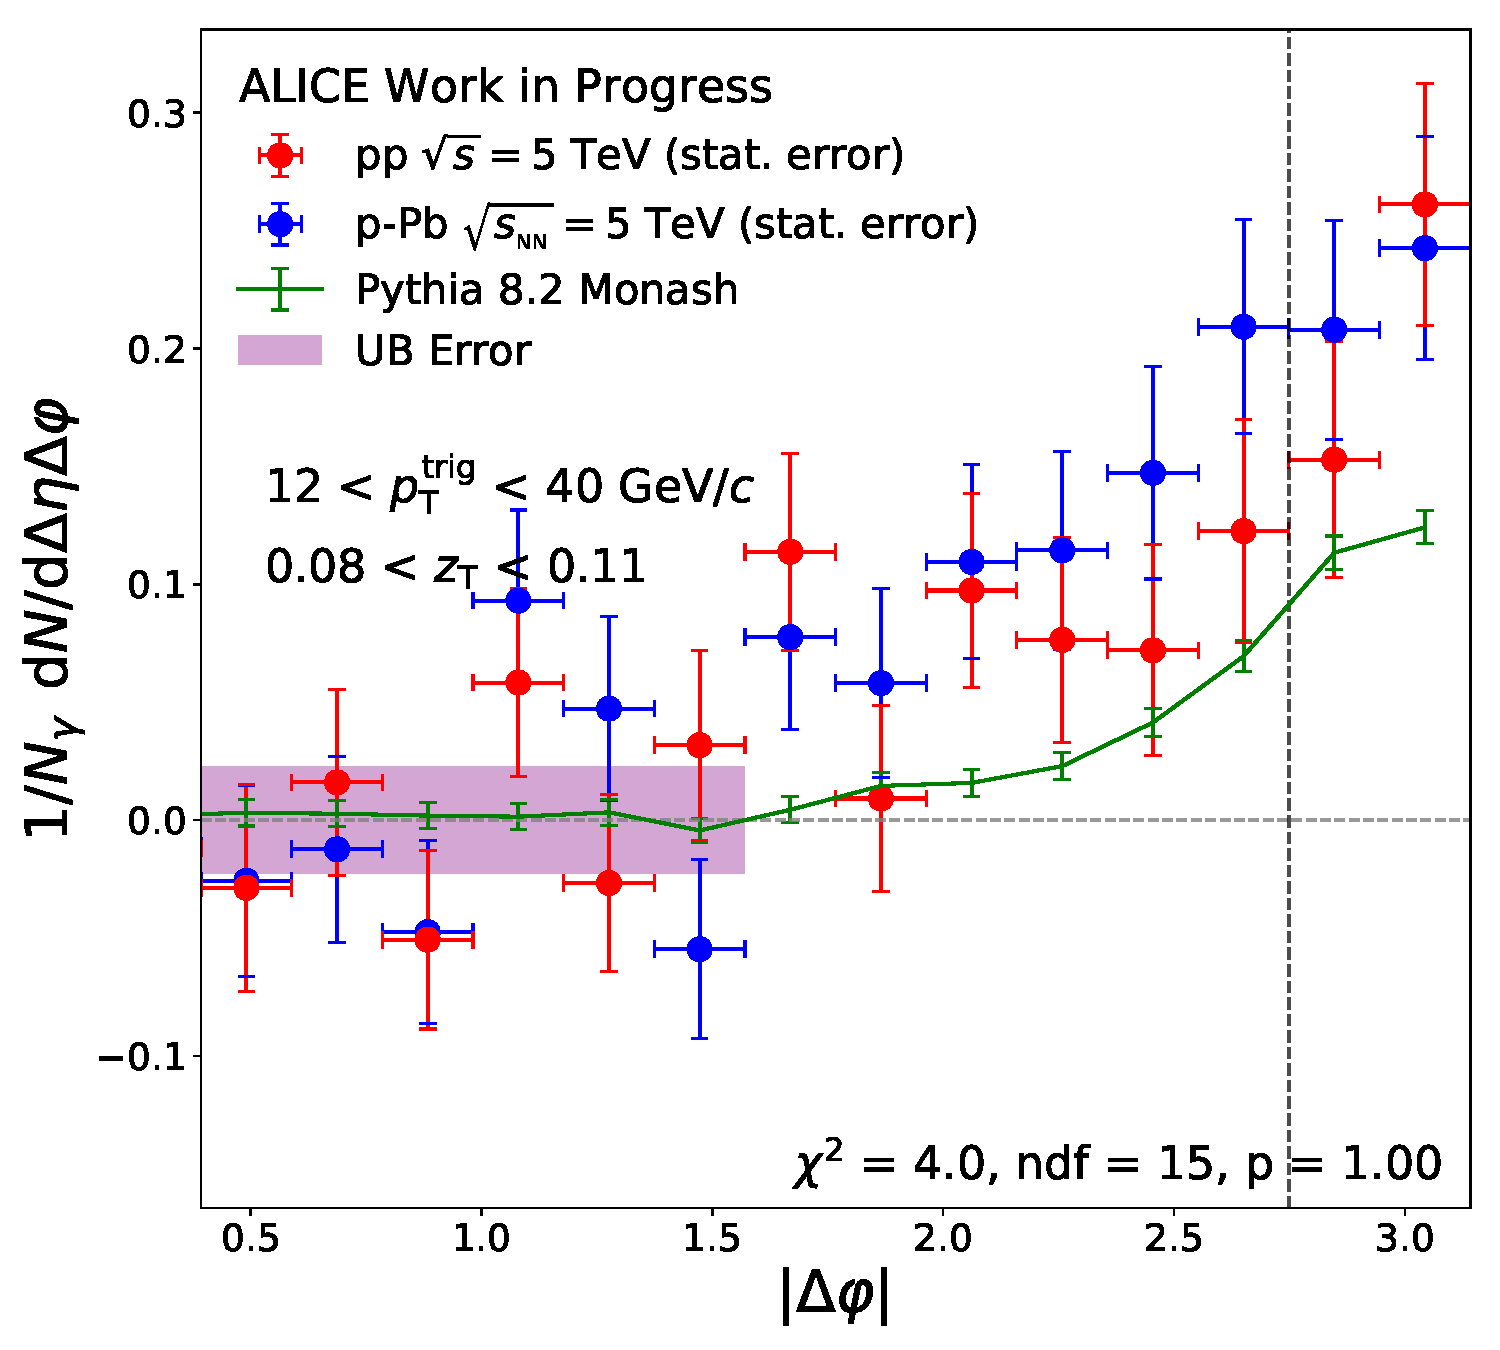
\includegraphics[width = 0.24 \textwidth]{G-H_New/16_dPhi/Cs_Final_Indv_pT_0_zT_1.pdf}
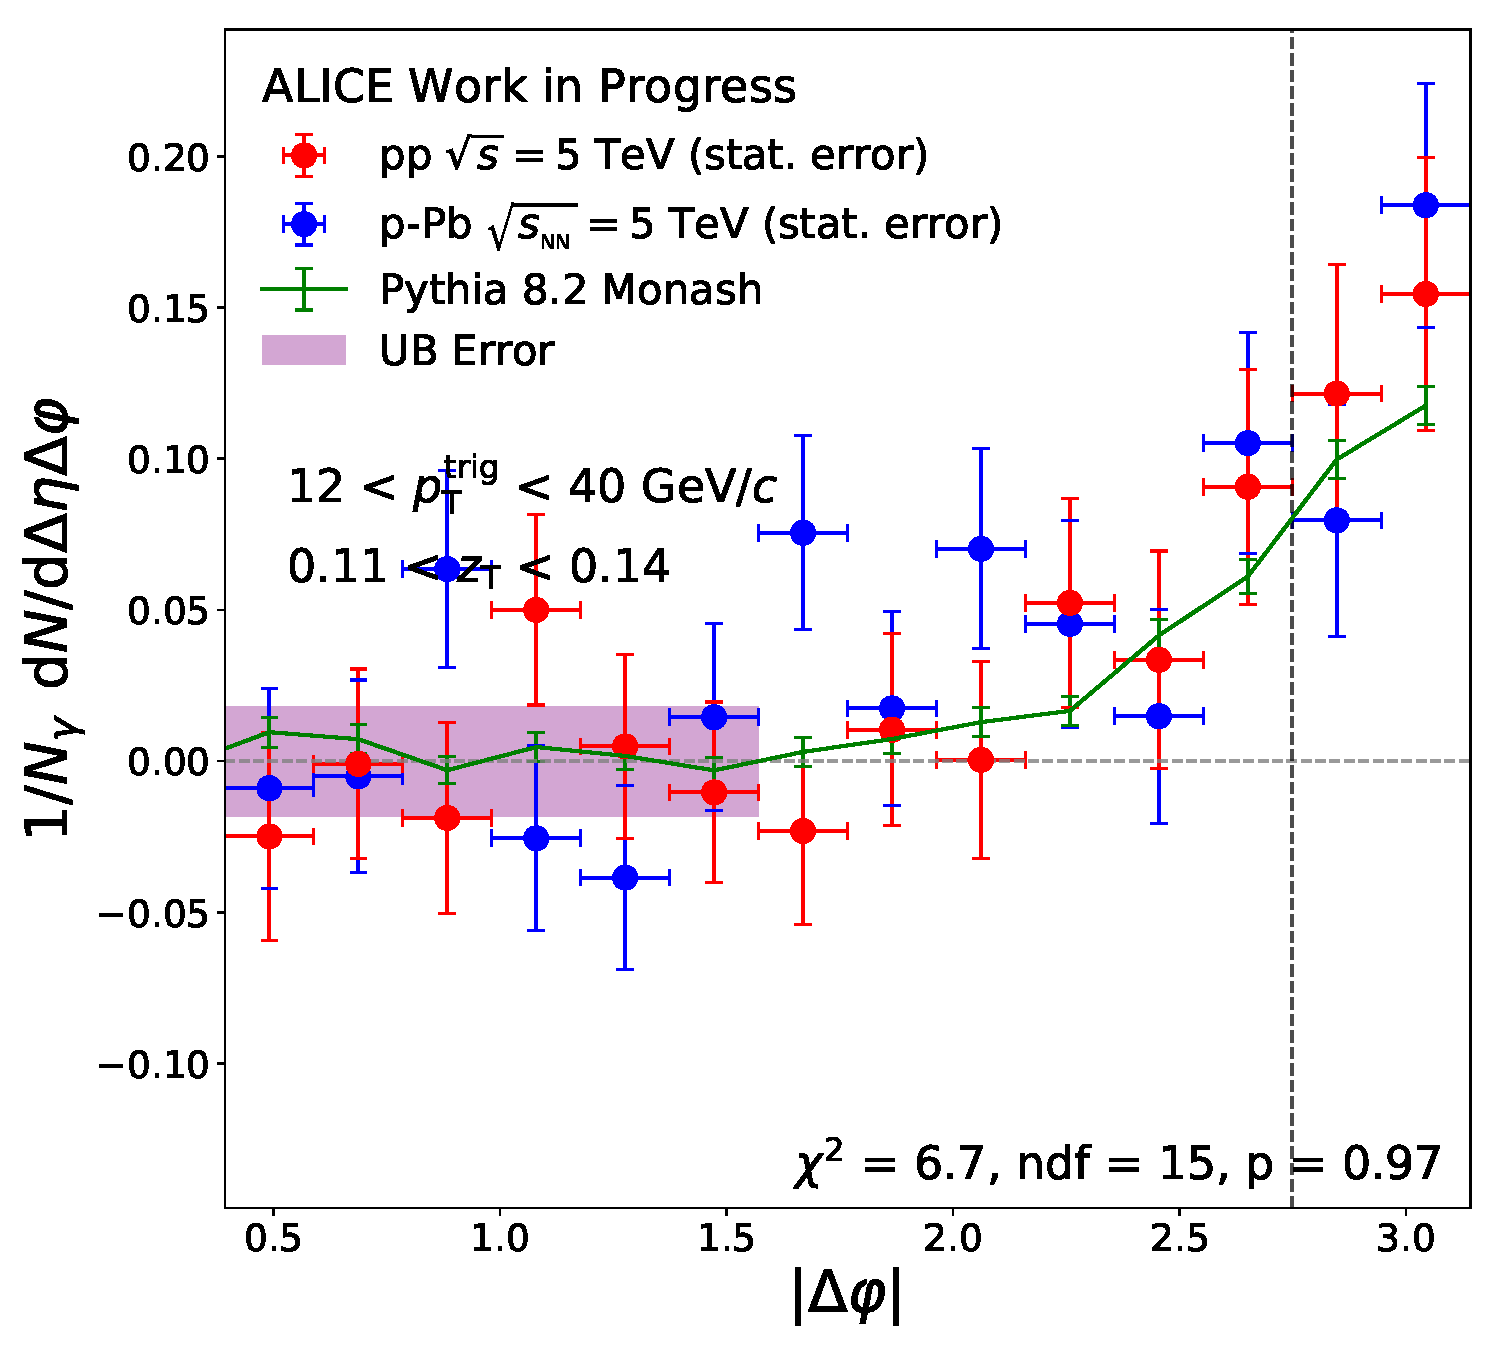
\includegraphics[width = 0.24 \textwidth]{G-H_New/16_dPhi/Cs_Final_Indv_pT_0_zT_2.pdf}
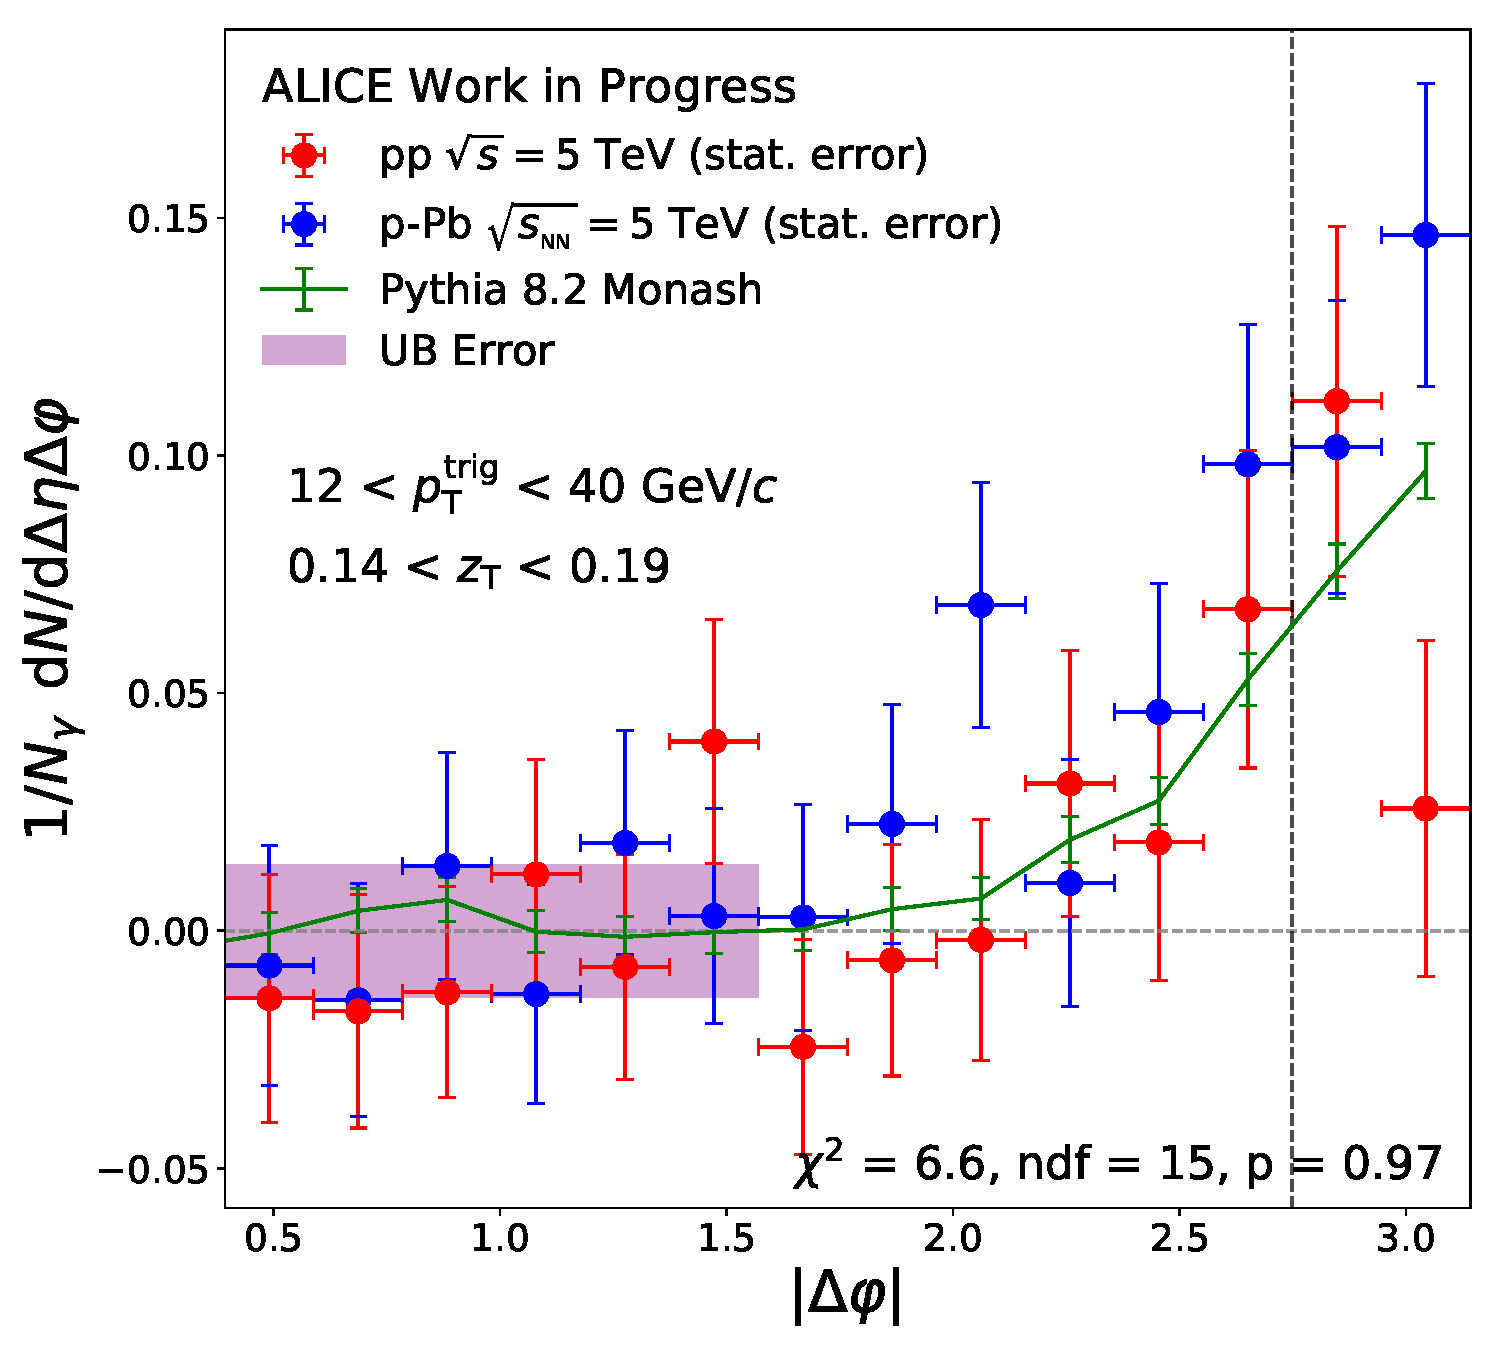
\includegraphics[width = 0.24 \textwidth]{G-H_New/16_dPhi/Cs_Final_Indv_pT_0_zT_3.pdf}
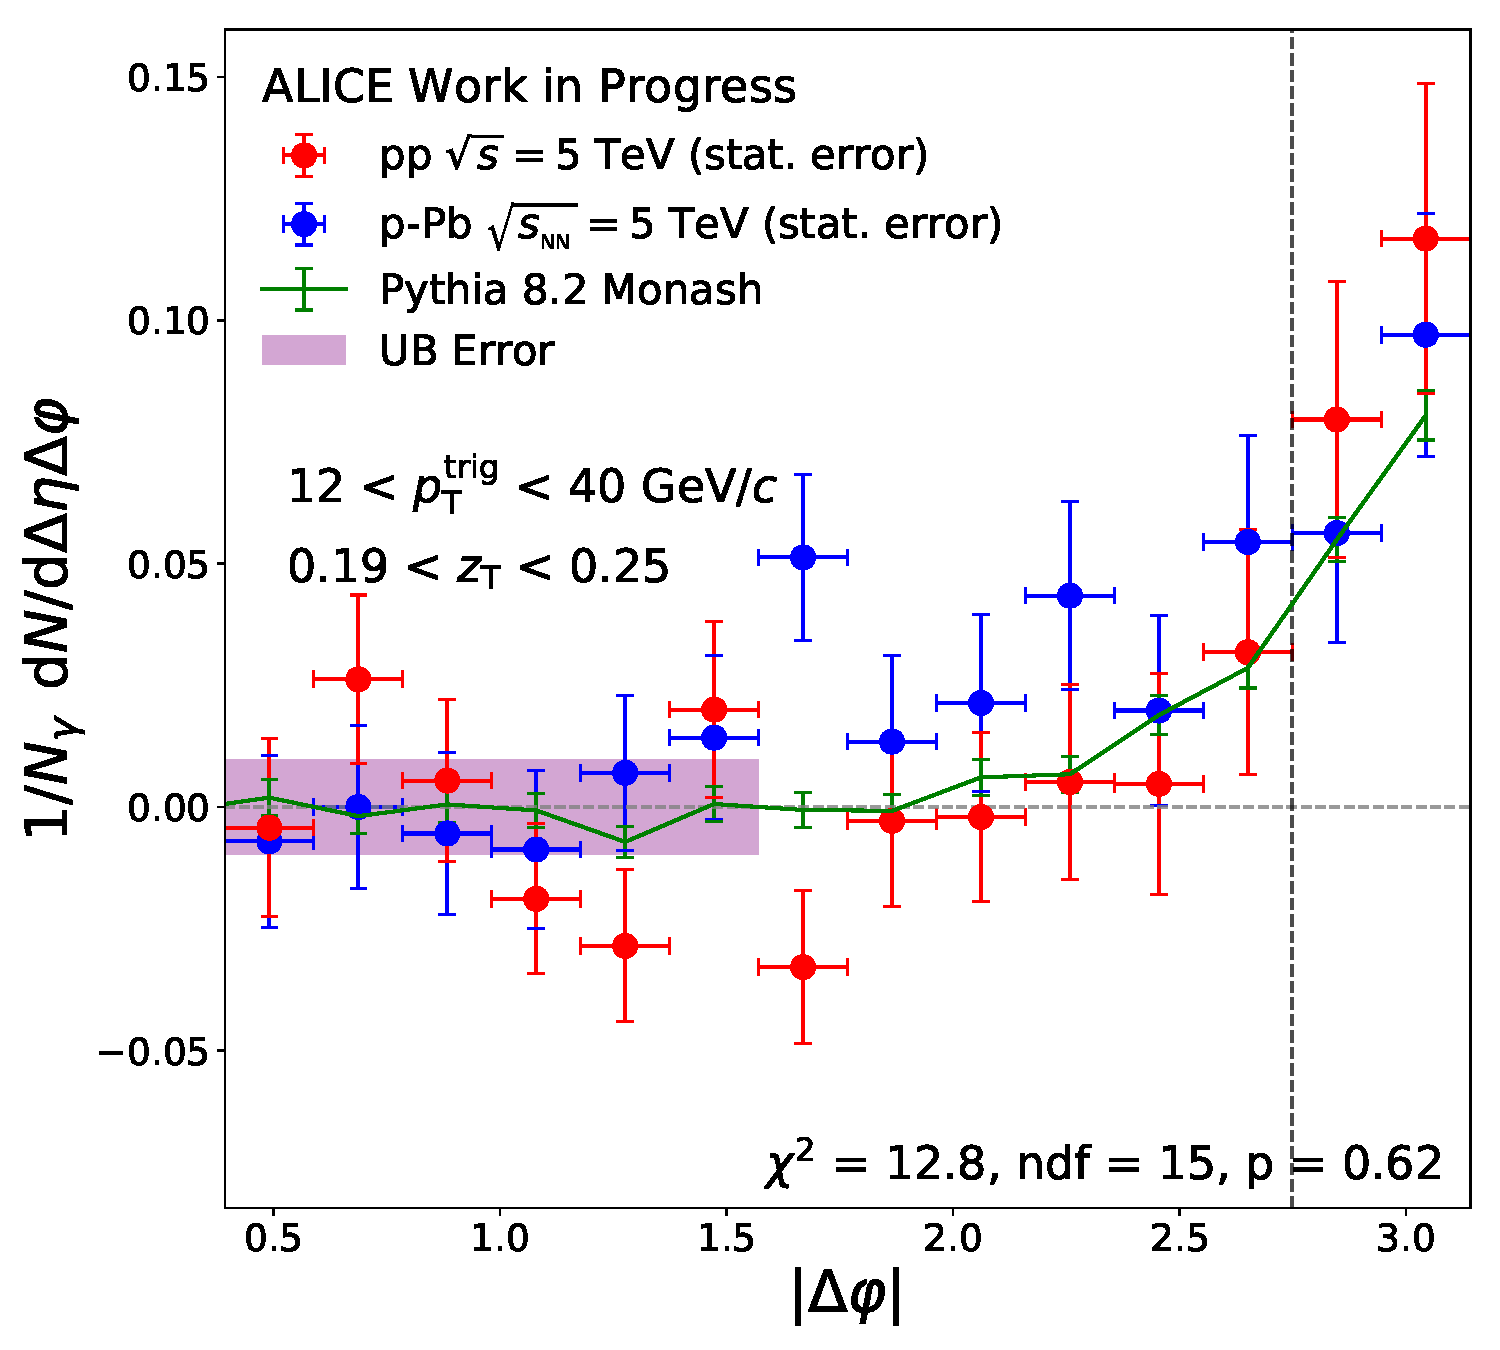
\includegraphics[width = 0.24 \textwidth]{G-H_New/16_dPhi/Cs_Final_Indv_pT_0_zT_4.pdf}
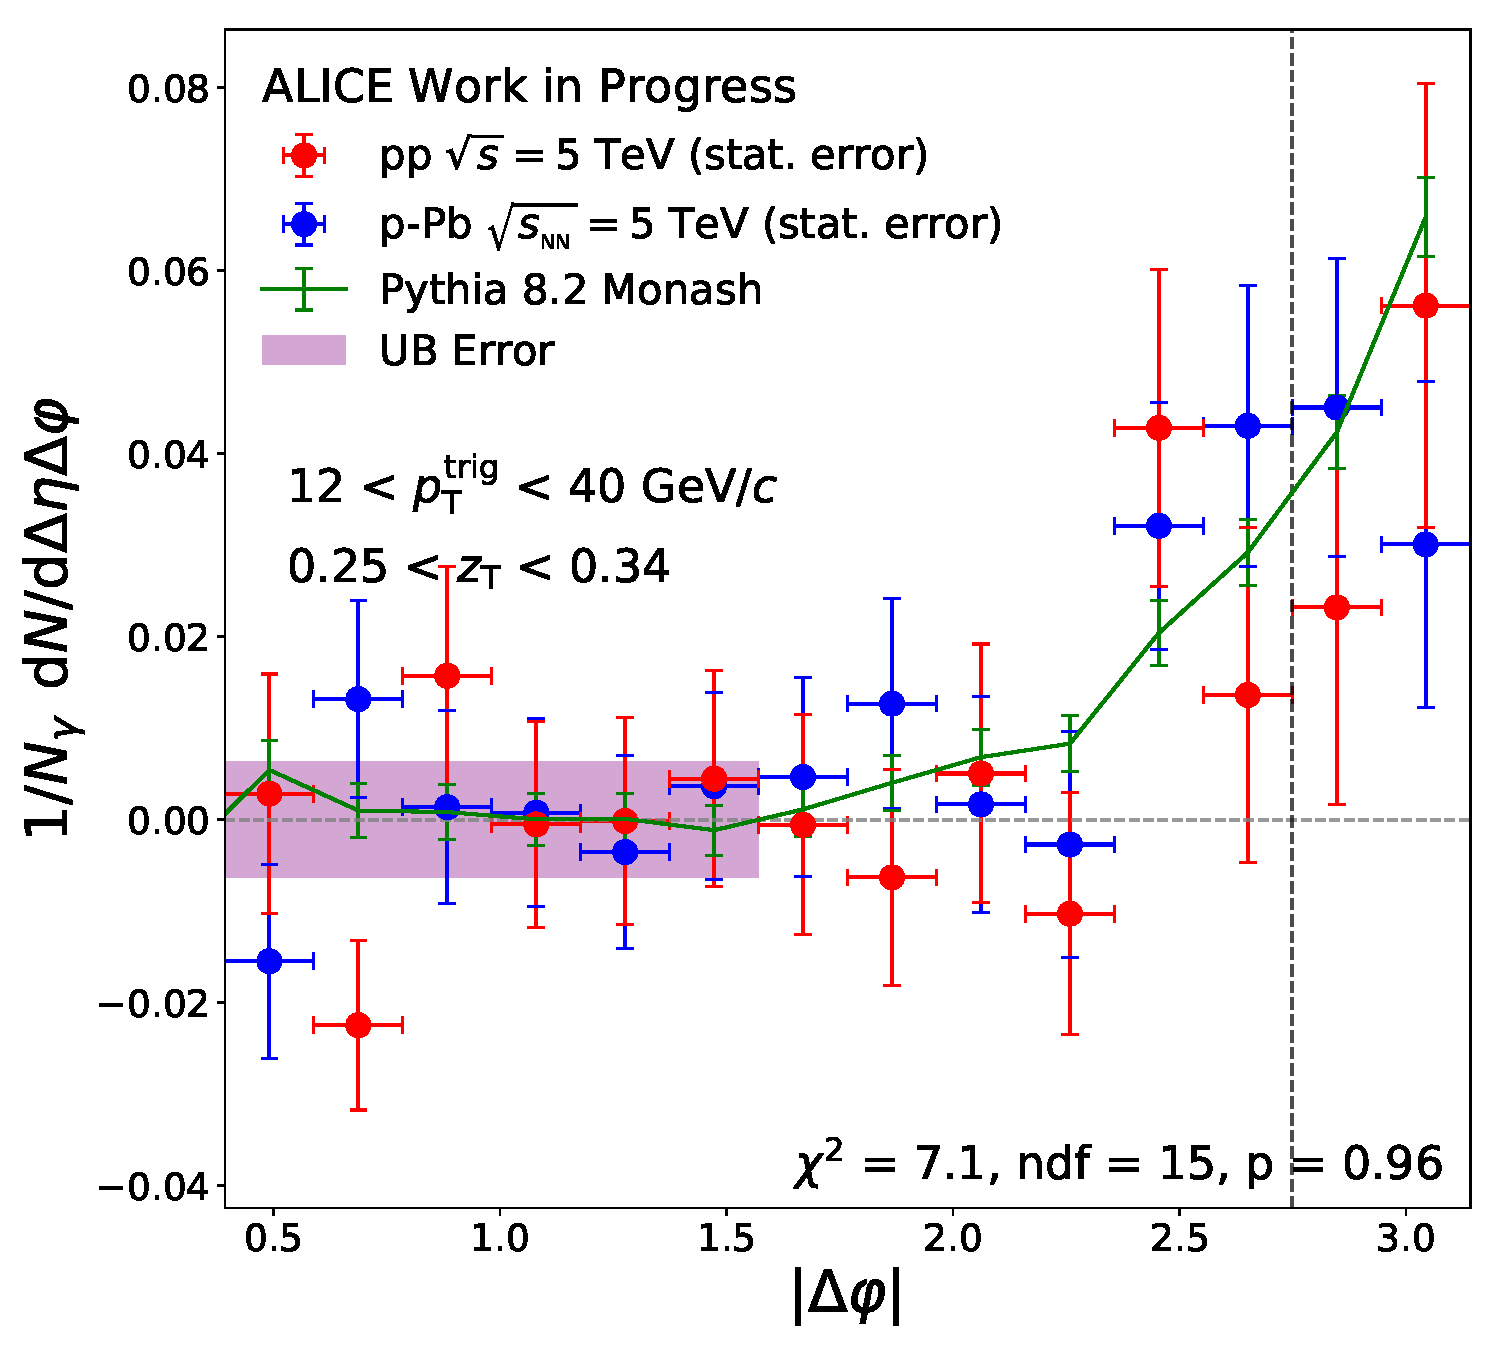
\includegraphics[width = 0.24 \textwidth]{G-H_New/16_dPhi/Cs_Final_Indv_pT_0_zT_5.pdf}
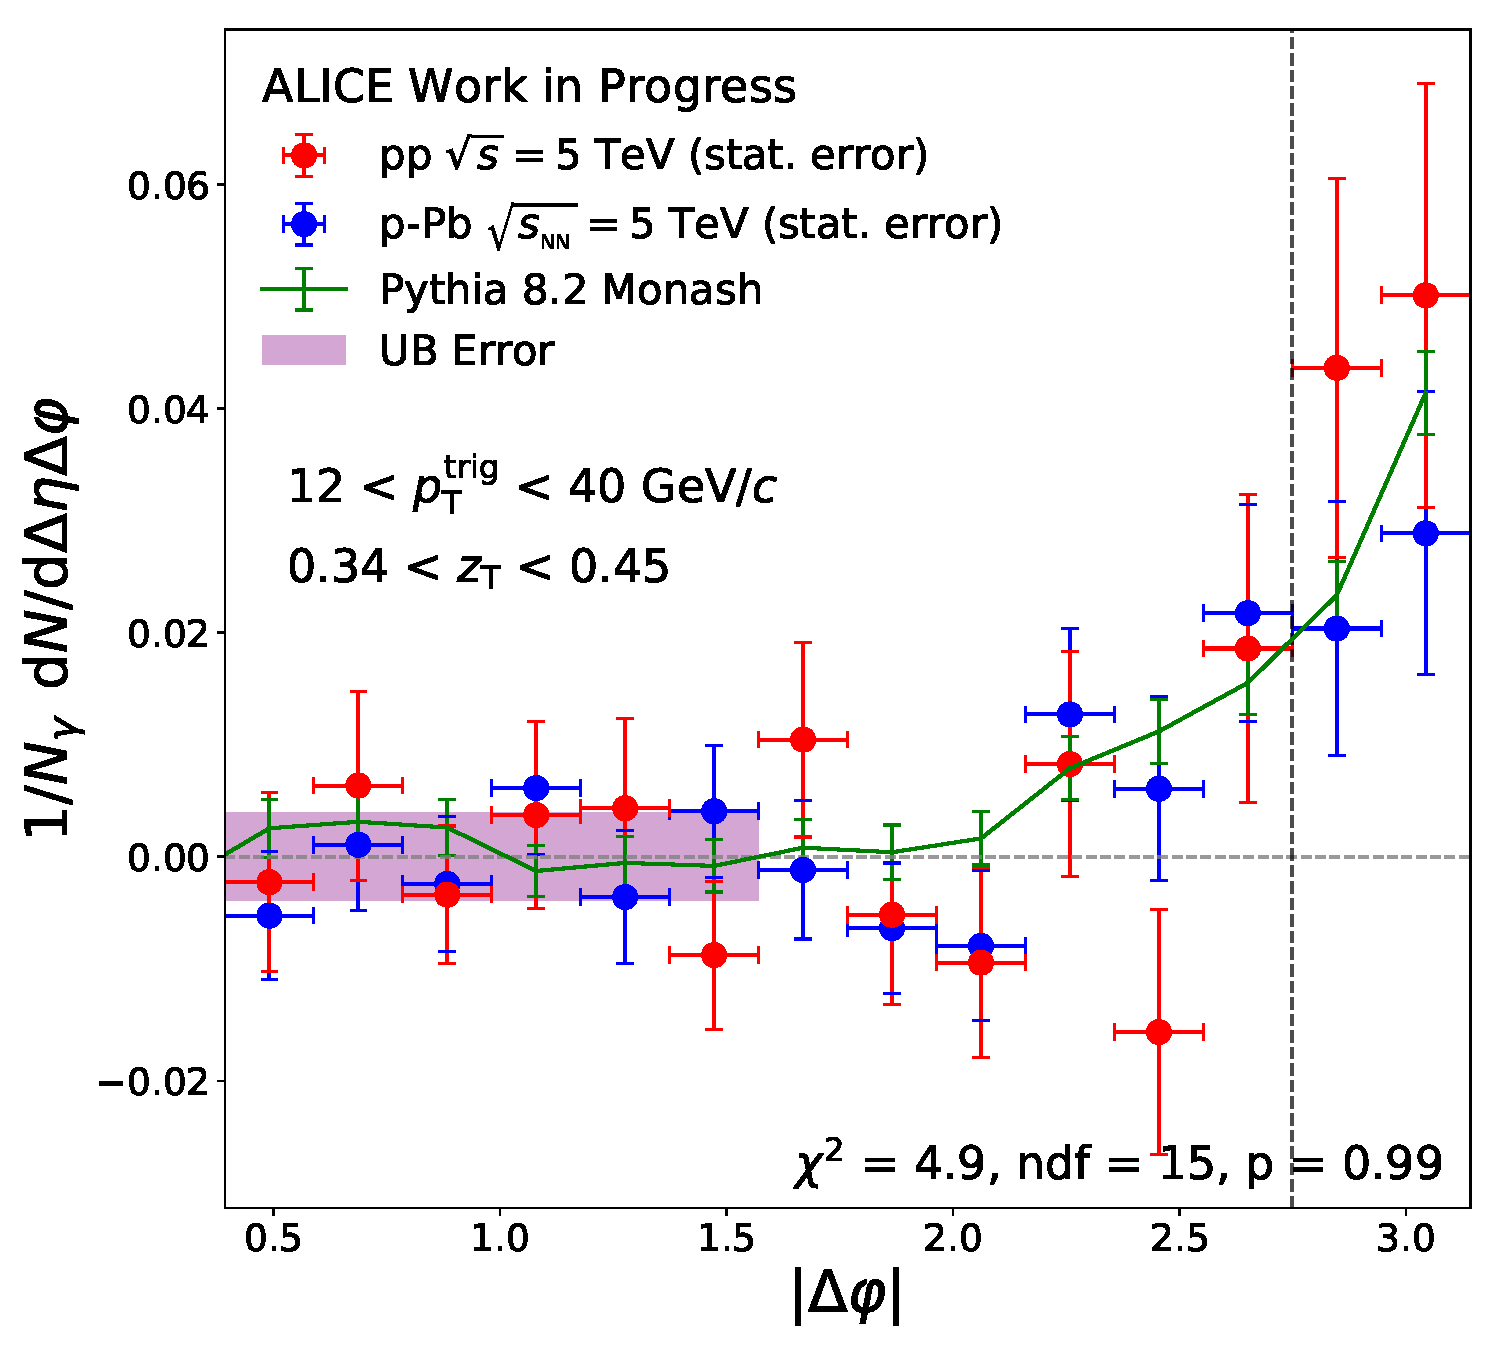
\includegraphics[width = 0.24 \textwidth]{G-H_New/16_dPhi/Cs_Final_Indv_pT_0_zT_6.pdf}
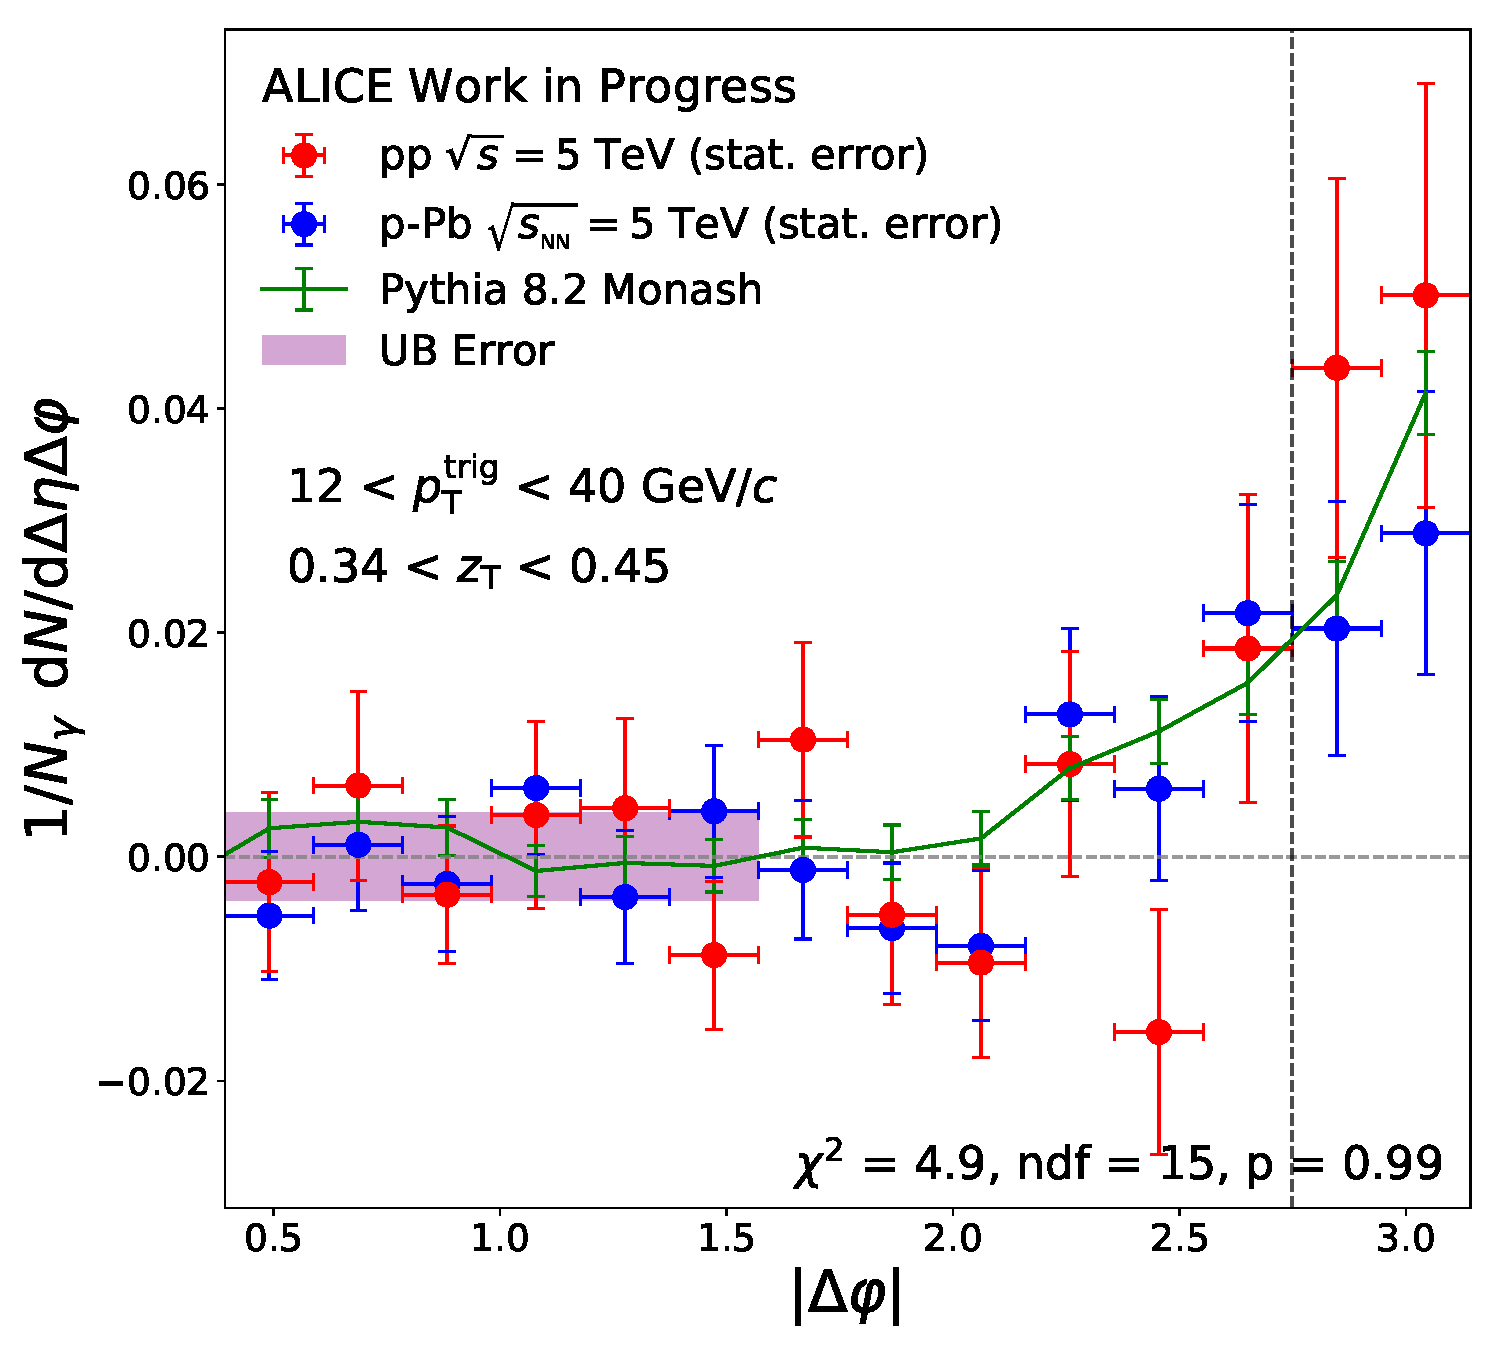
\includegraphics[width = 0.24 \textwidth]{G-H_New/16_dPhi/Cs_Final_Indv_pT_0_zT_6.pdf}
\caption{Fully-corrected $\gammaiso$--hadron correlation function pp (red) and \pPb~(blue) data. The purple band represents the uncertainty from the underlying event estimate in pp and \pPb. The error bars represent statistical uncertainty only. The green line is the \gammaiso--hadron correlation function obtained with \textsc{PYTHIA 8.2}. This difference with the nominal results shown in Section~\ref{sec:results} is that here we double the number of $\Delta\varphi$ bins.}
\end{sidewaysfigure}

%\begin{figure}
%\centering
%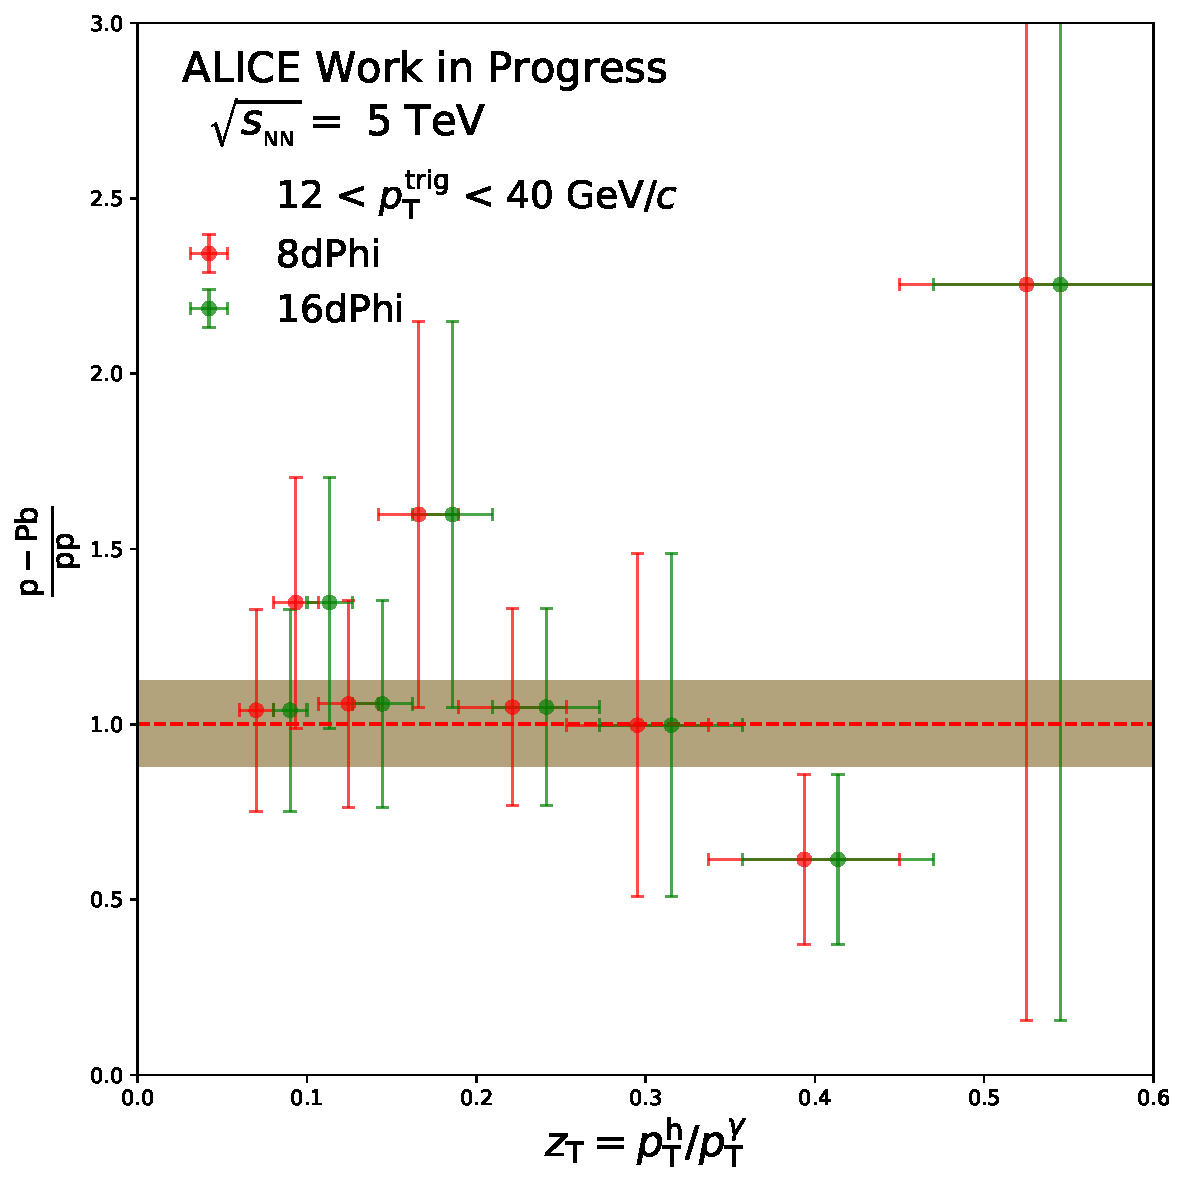
\includegraphics[width = 0.49 \textwidth]{G-H_New/16_dPhi/Ratio_FF_Averages_Phi_Rebinning}
%\caption{Comparison of ratio of fragmentation functions with different $\Delta\varphi$ binning.}
%\label{fig:dPhiRatio}
%\end{figure}

\section{Checking Sensitivity to Beam Flip}
Figure~\ref{fig:Cs_Beam_Flip} shows results for 13de and 13f periods. They differ in the beam configuration and have roughly similar integrated luminosity. We observe no significant difference. 

\begin{figure}
\centering
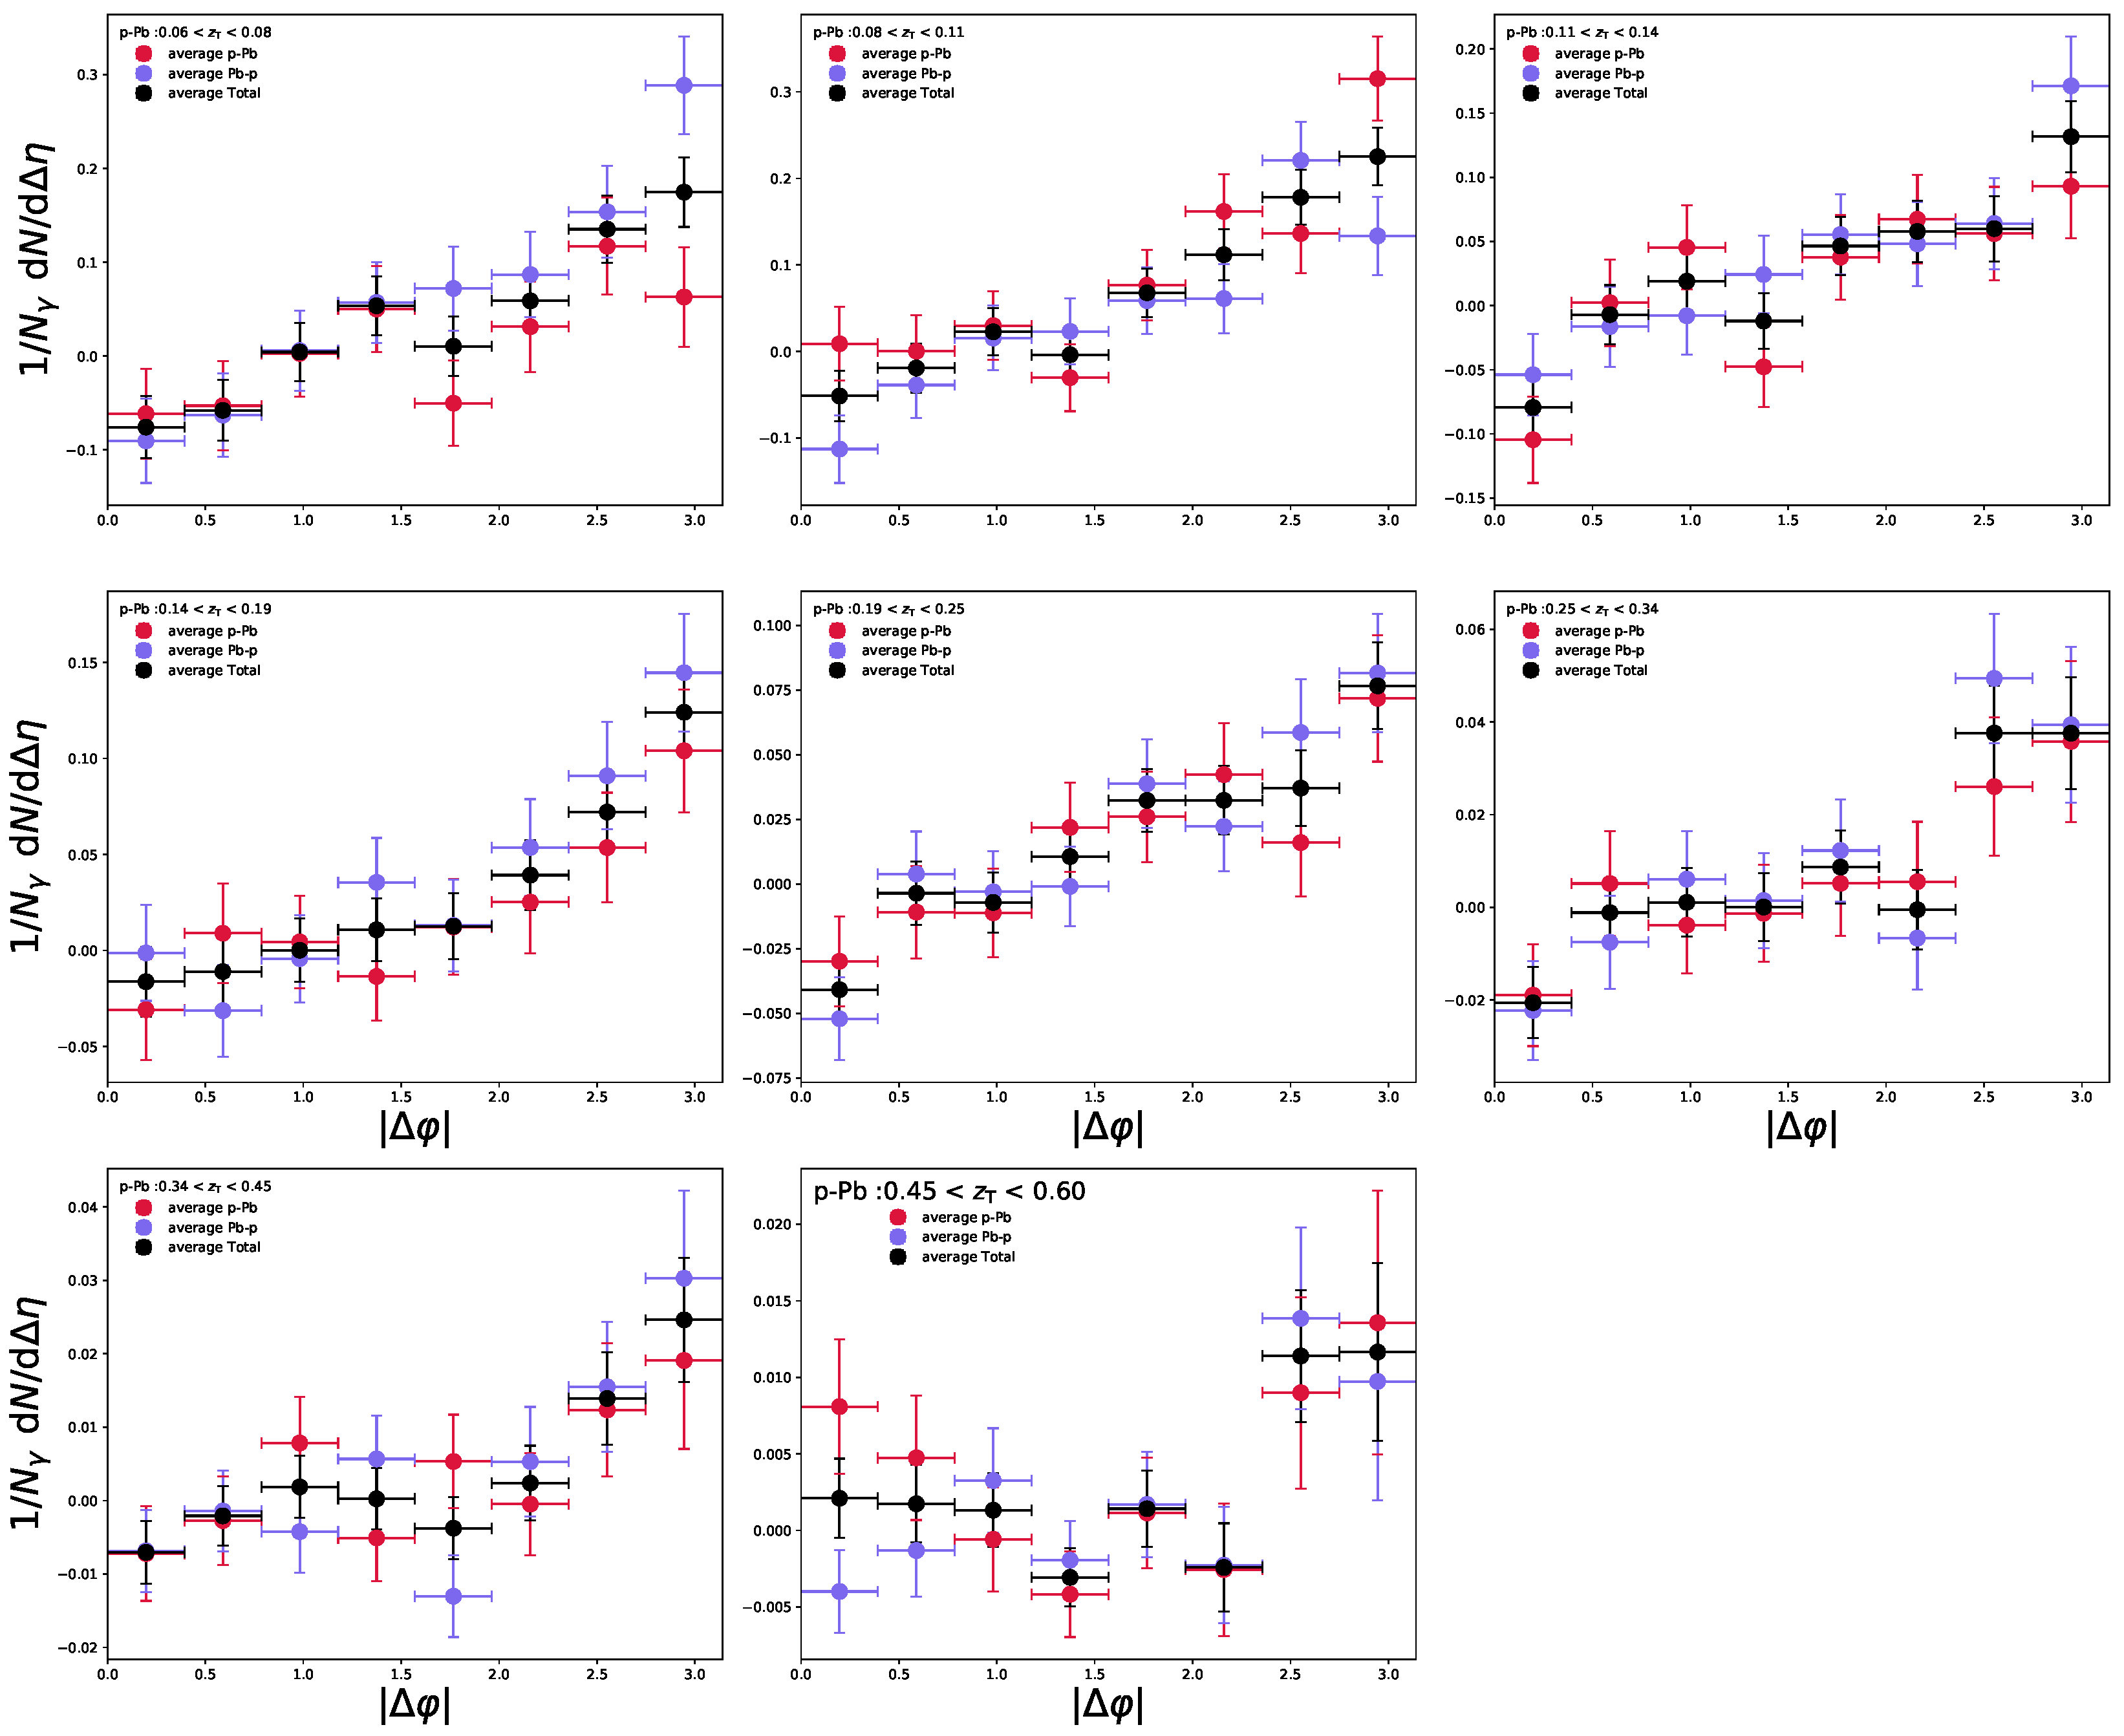
\includegraphics[width = 0.9 \textwidth]{G-H_New/Cs_Averages_p-Pb_Beam_Flip.pdf}
\caption{Comparison of final correlations functions for p--Pb (red) and Pb--p (blue) collisions.}
\label{fig:Cs_Beam_Flip}
\end{figure}



\section{Correlations including $\Delta\varphi=0$ }
Figure~\ref{fig:CorrelationFinal_downtozero} shows the correlation results down to 0 radians. The first bin is contained within the isolation requirement and therefore is biased, which is why we chose to not report it in our main results. 

\begin{sidewaysfigure}
\centering
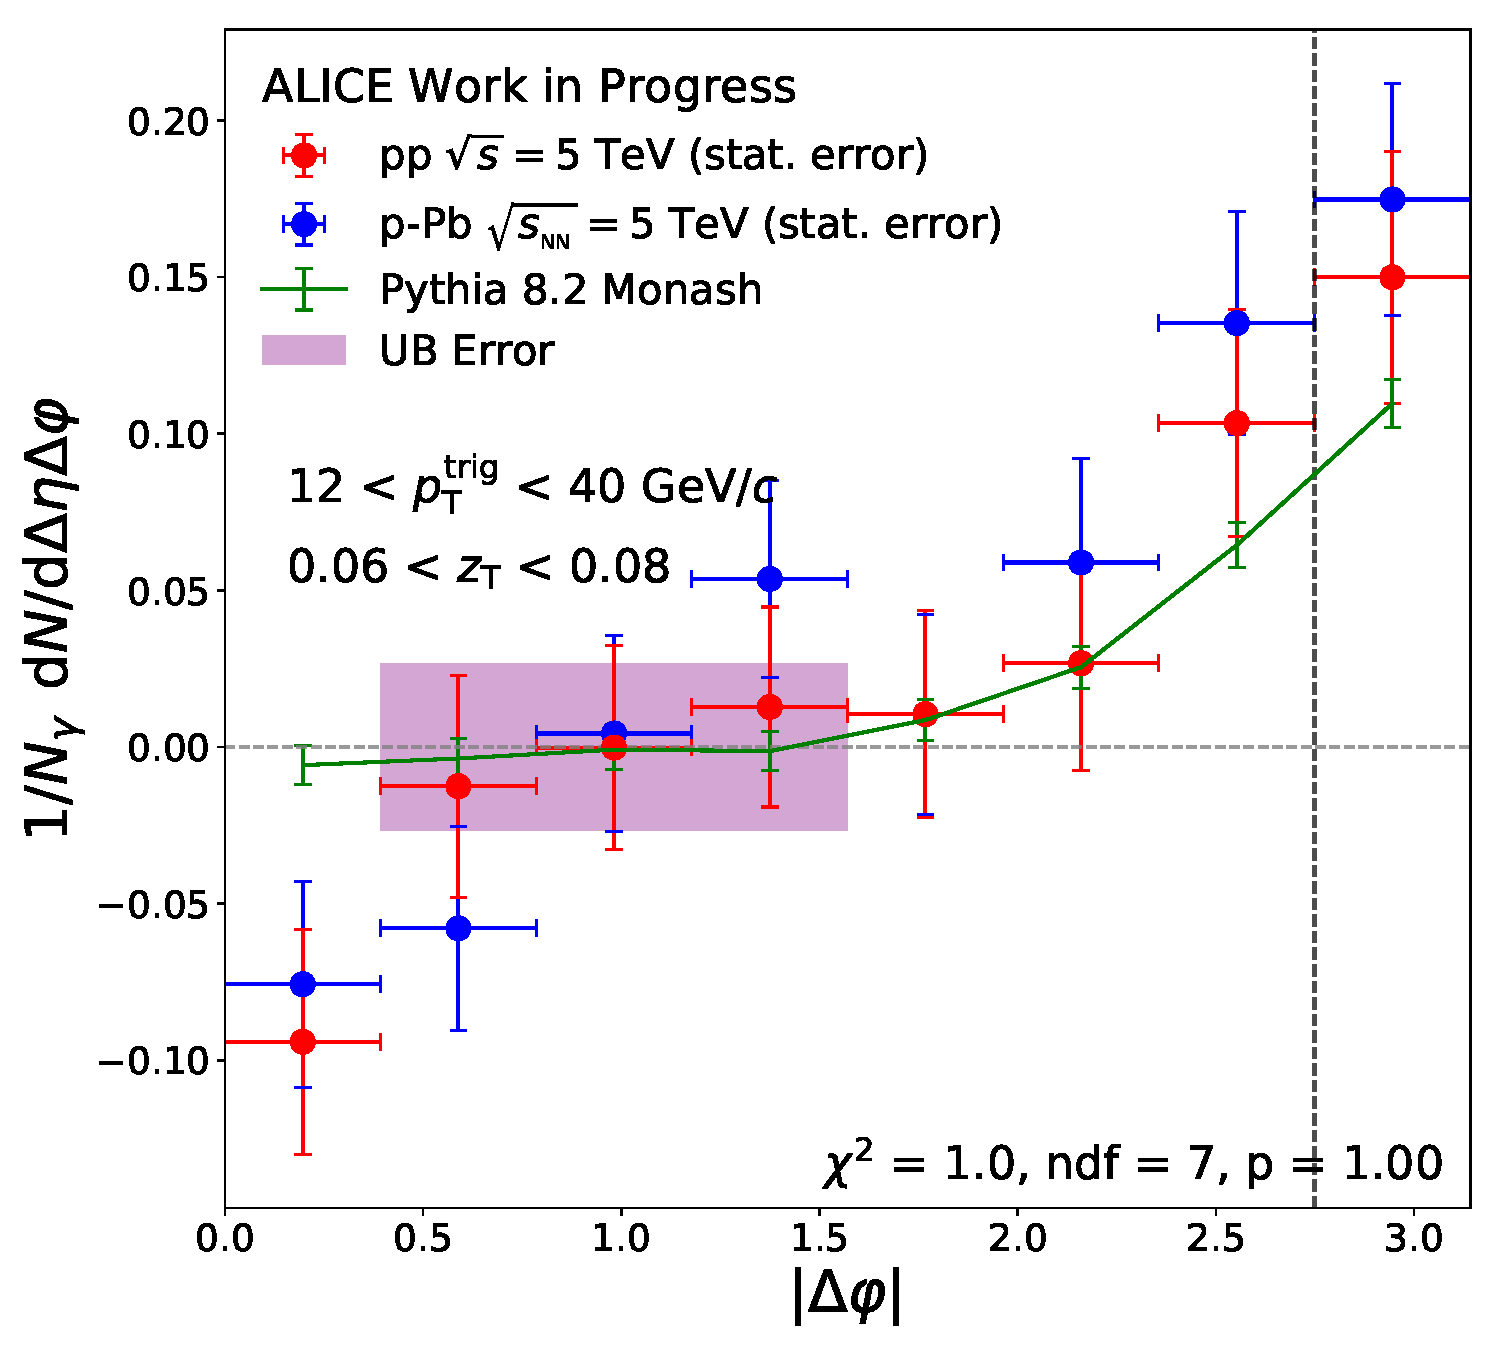
\includegraphics[width = 0.24 \textwidth]{G-H_New/dPhi_to_0/Cs_Final_Indv_pT_0_zT_0.pdf}
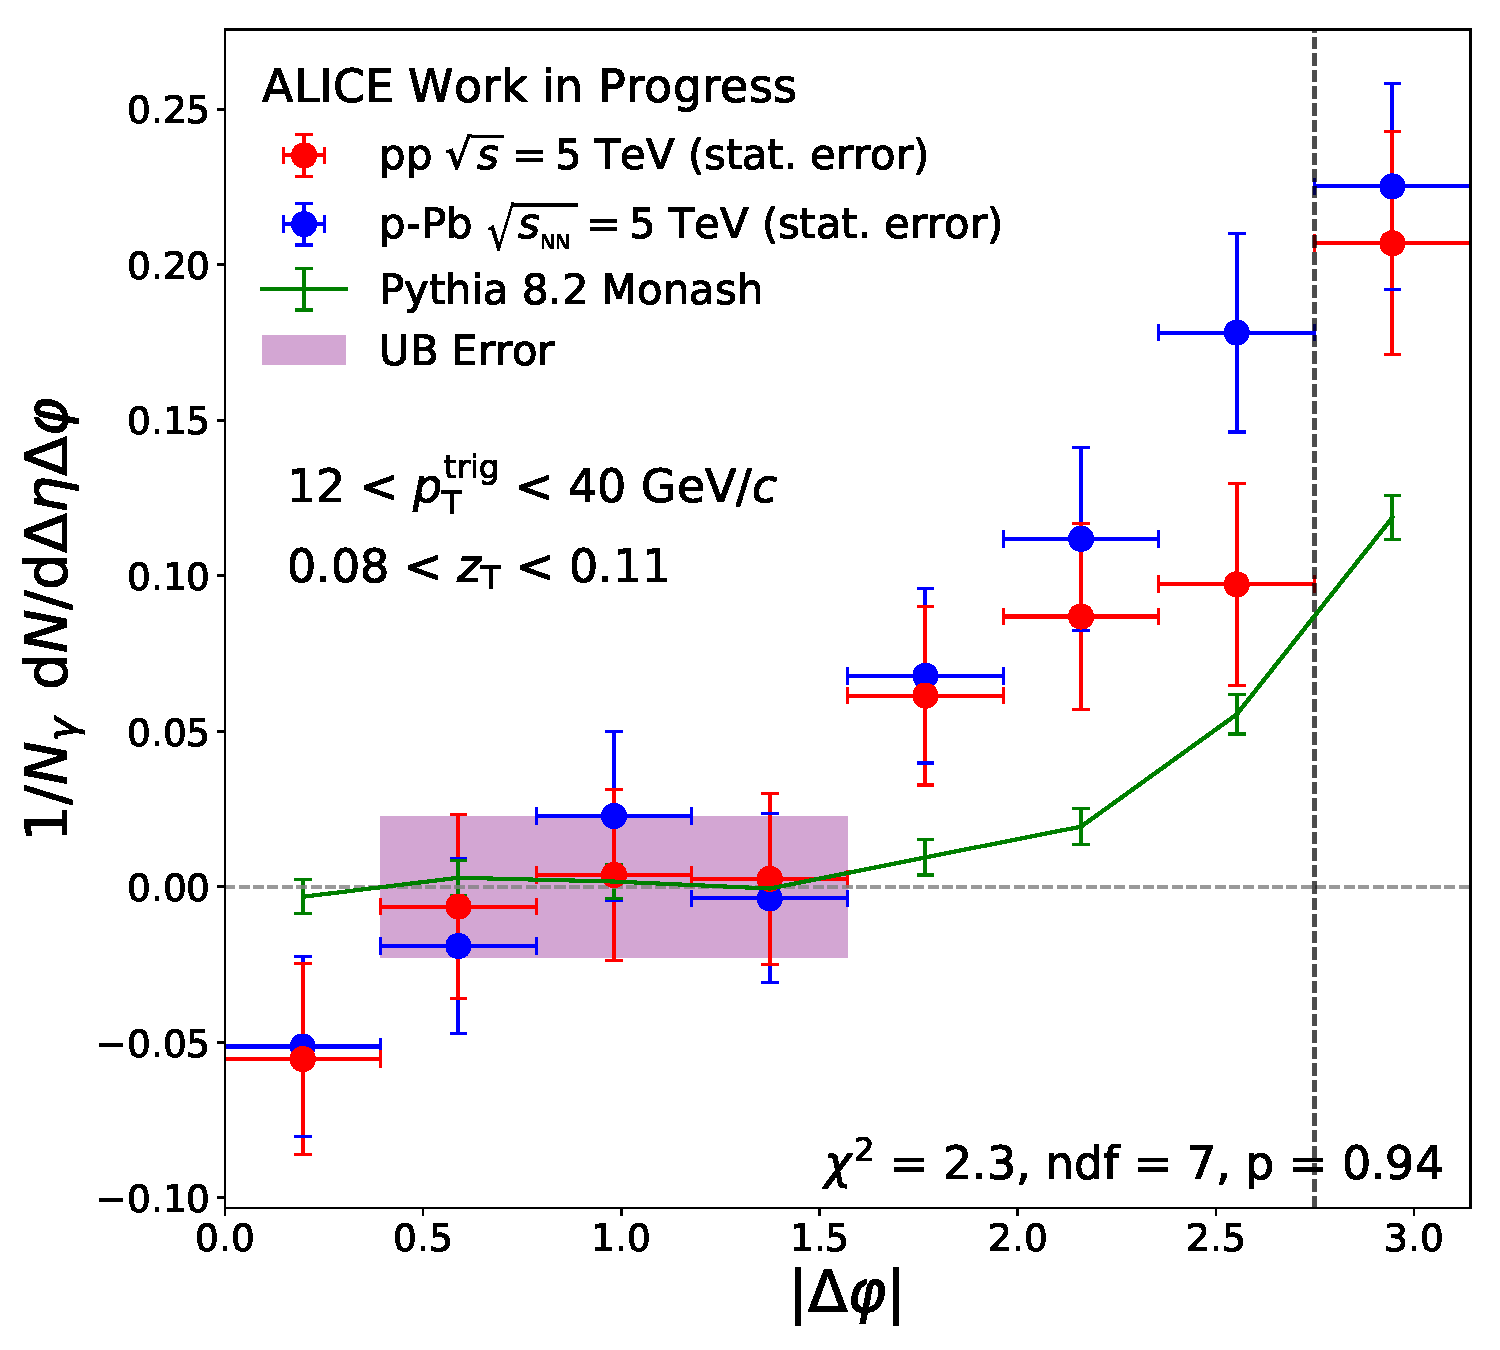
\includegraphics[width = 0.24 \textwidth]{G-H_New/dPhi_to_0/Cs_Final_Indv_pT_0_zT_1.pdf}
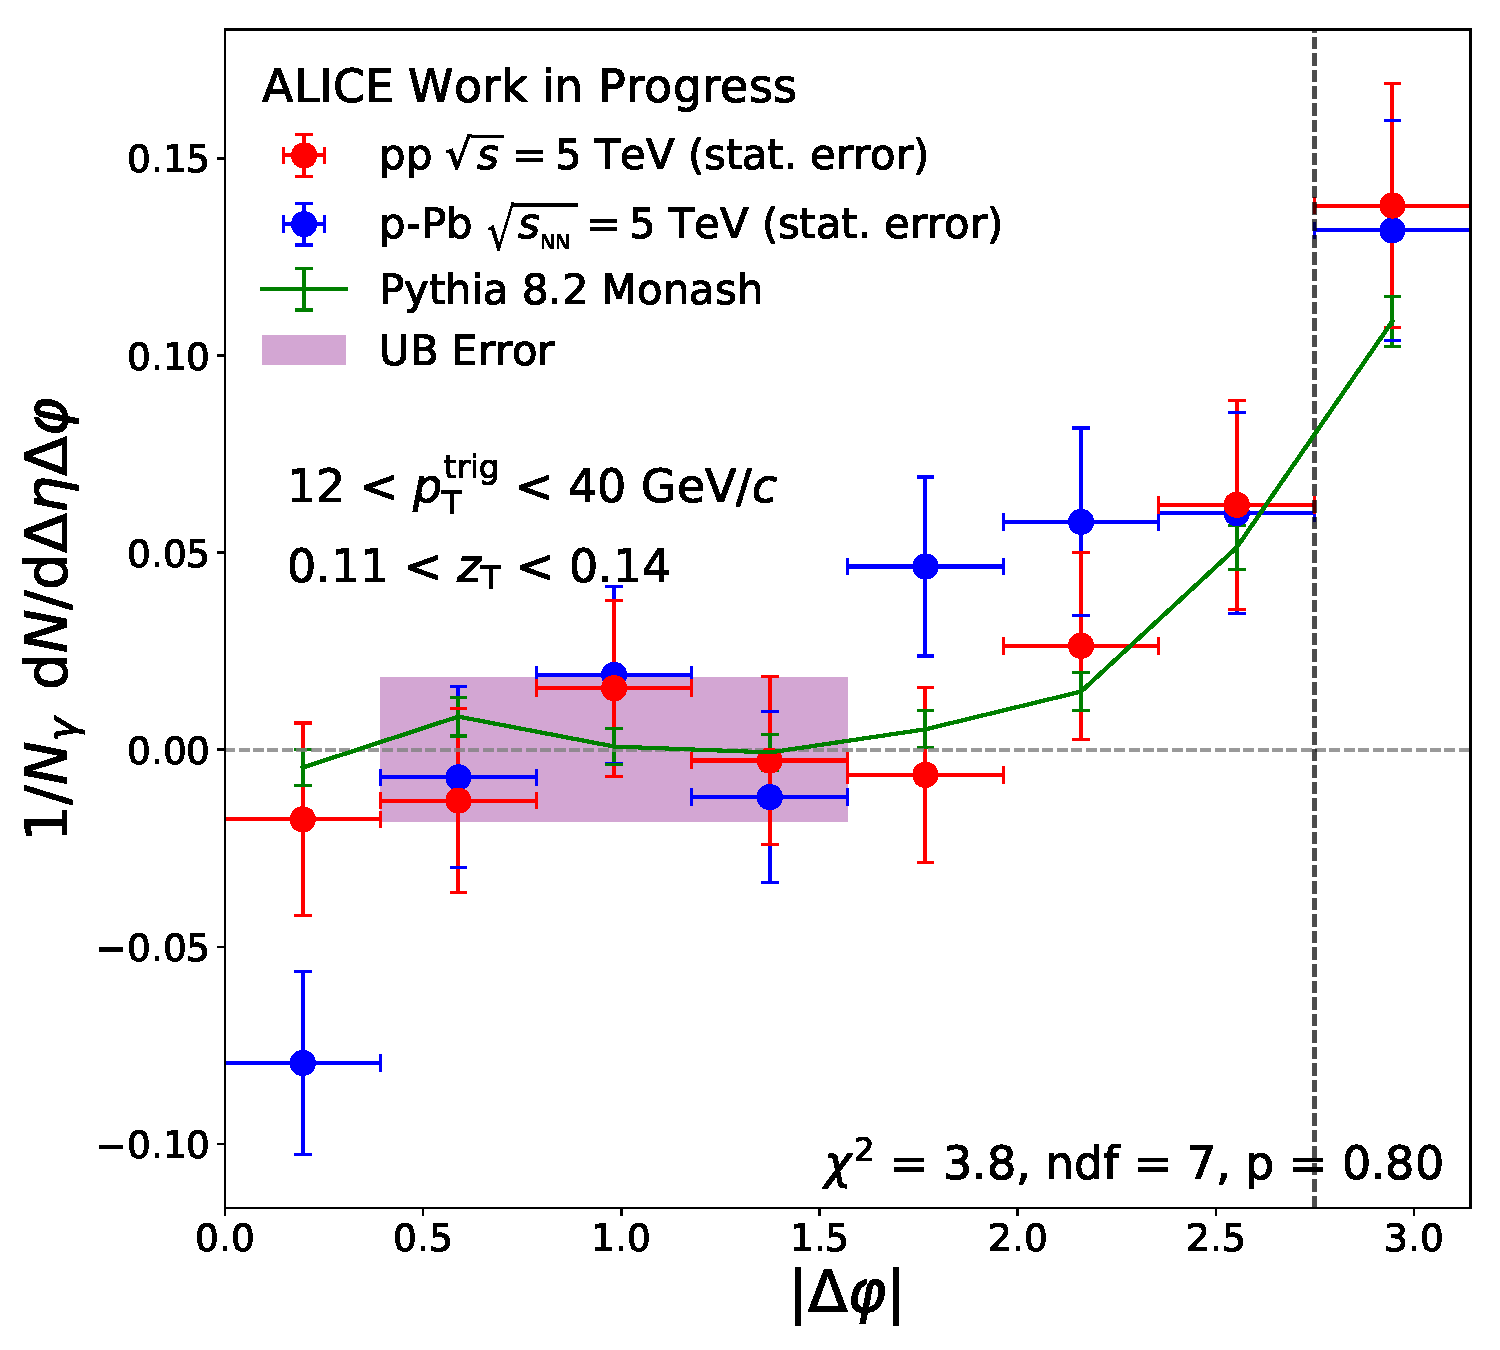
\includegraphics[width = 0.24 \textwidth]{G-H_New/dPhi_to_0/Cs_Final_Indv_pT_0_zT_2.pdf}
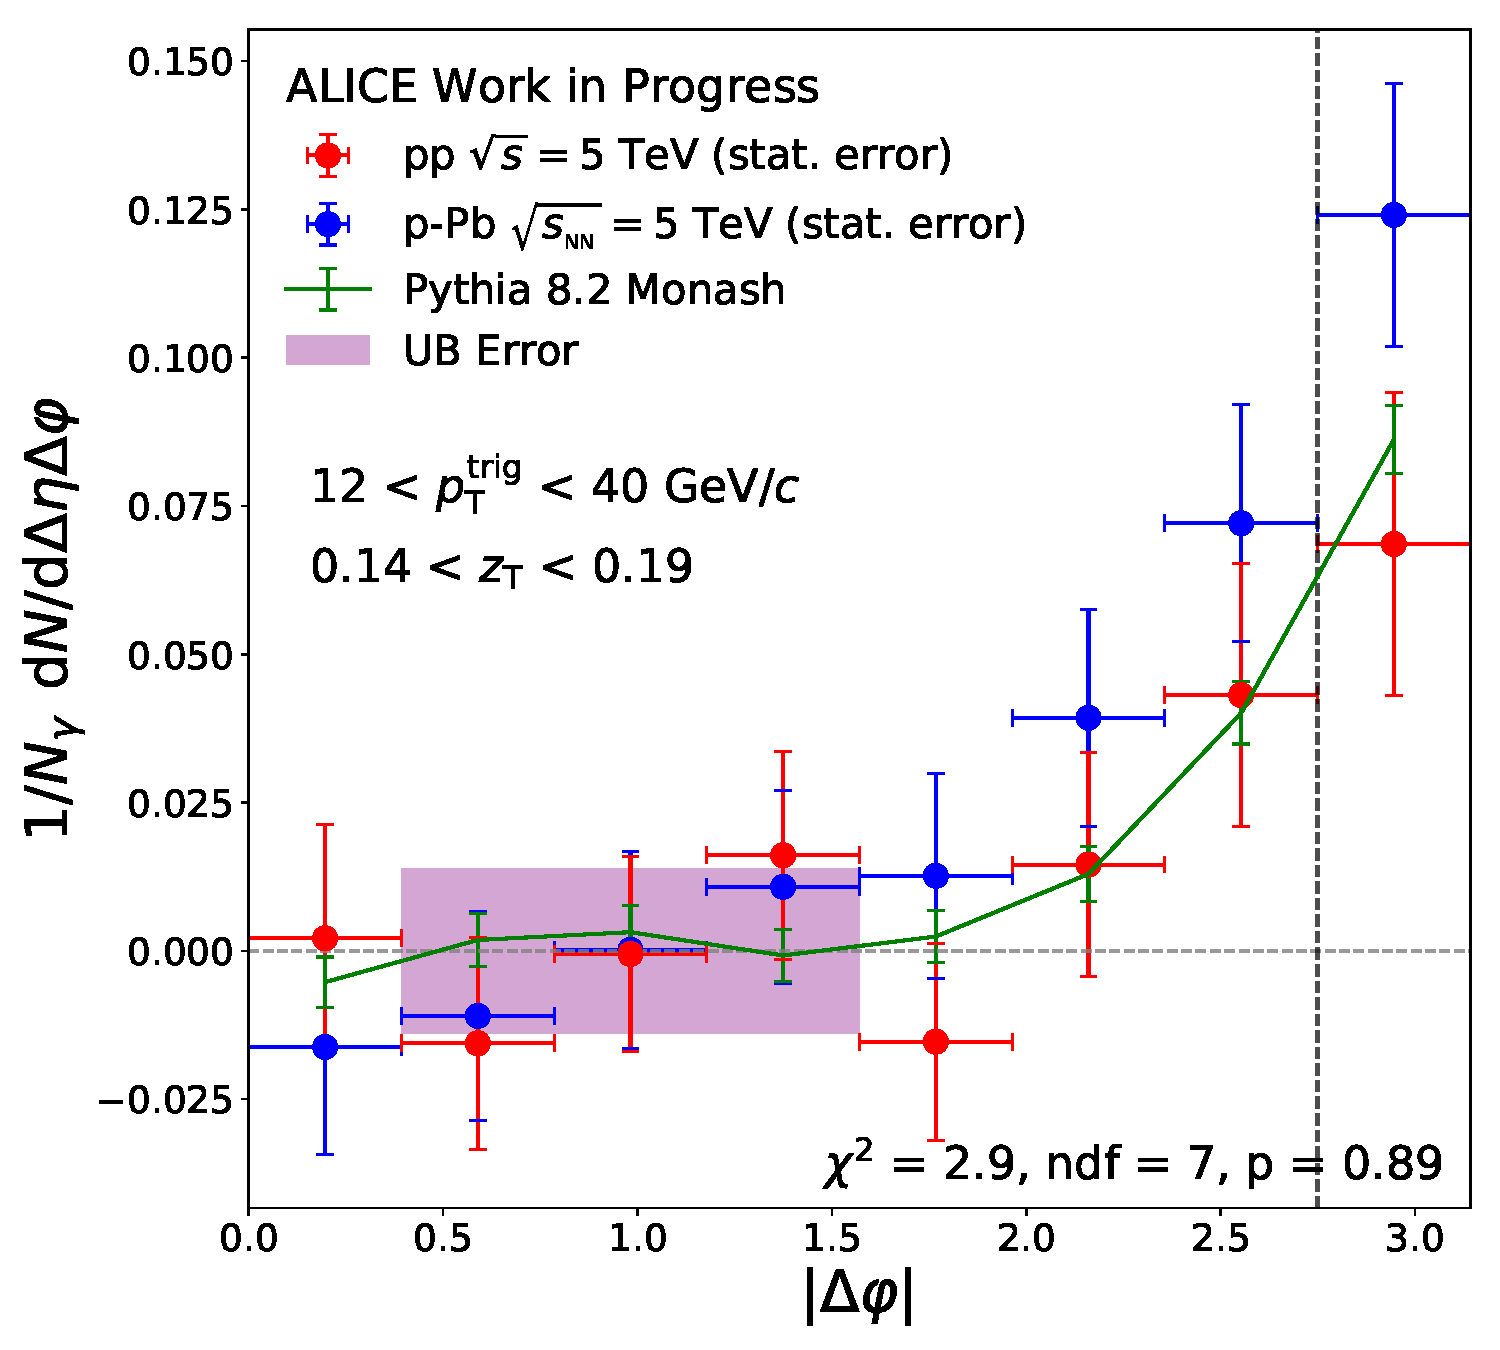
\includegraphics[width = 0.24 \textwidth]{G-H_New/dPhi_to_0/Cs_Final_Indv_pT_0_zT_3.pdf}
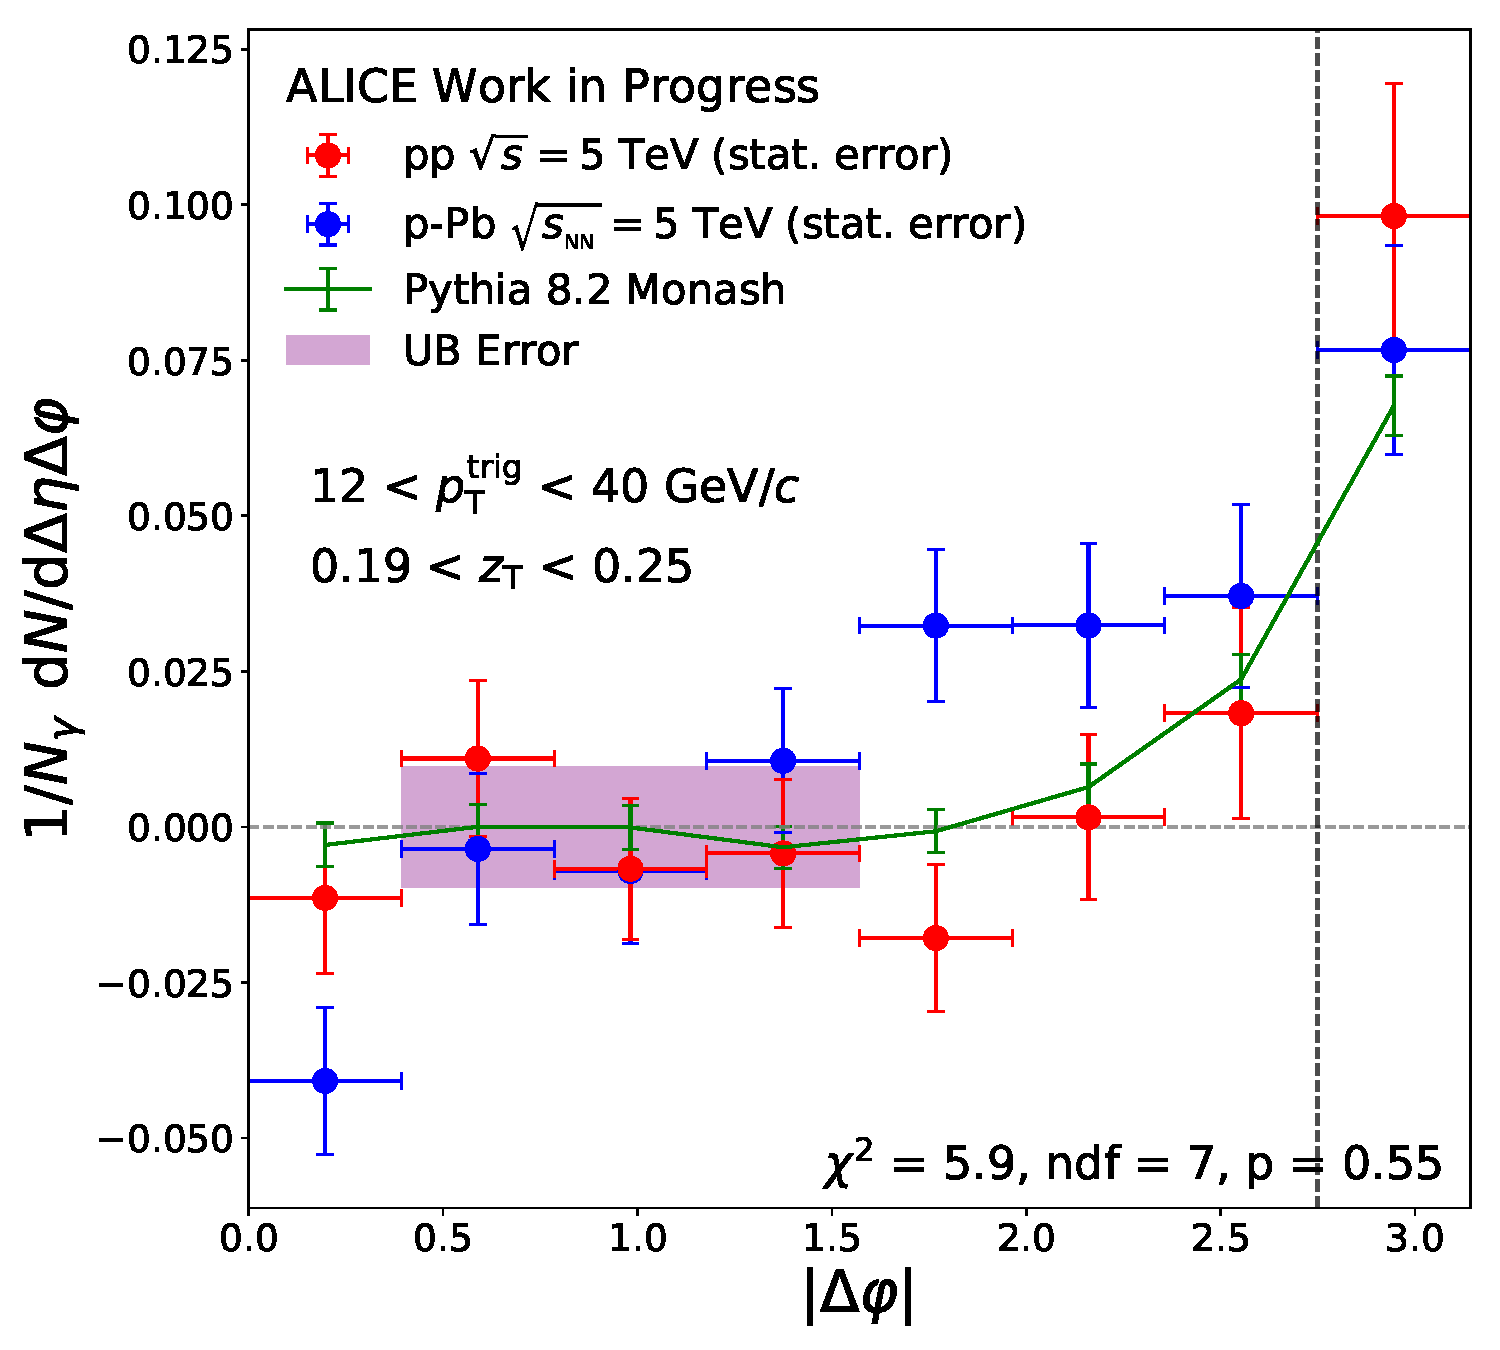
\includegraphics[width = 0.24 \textwidth]{G-H_New/dPhi_to_0/Cs_Final_Indv_pT_0_zT_4.pdf}
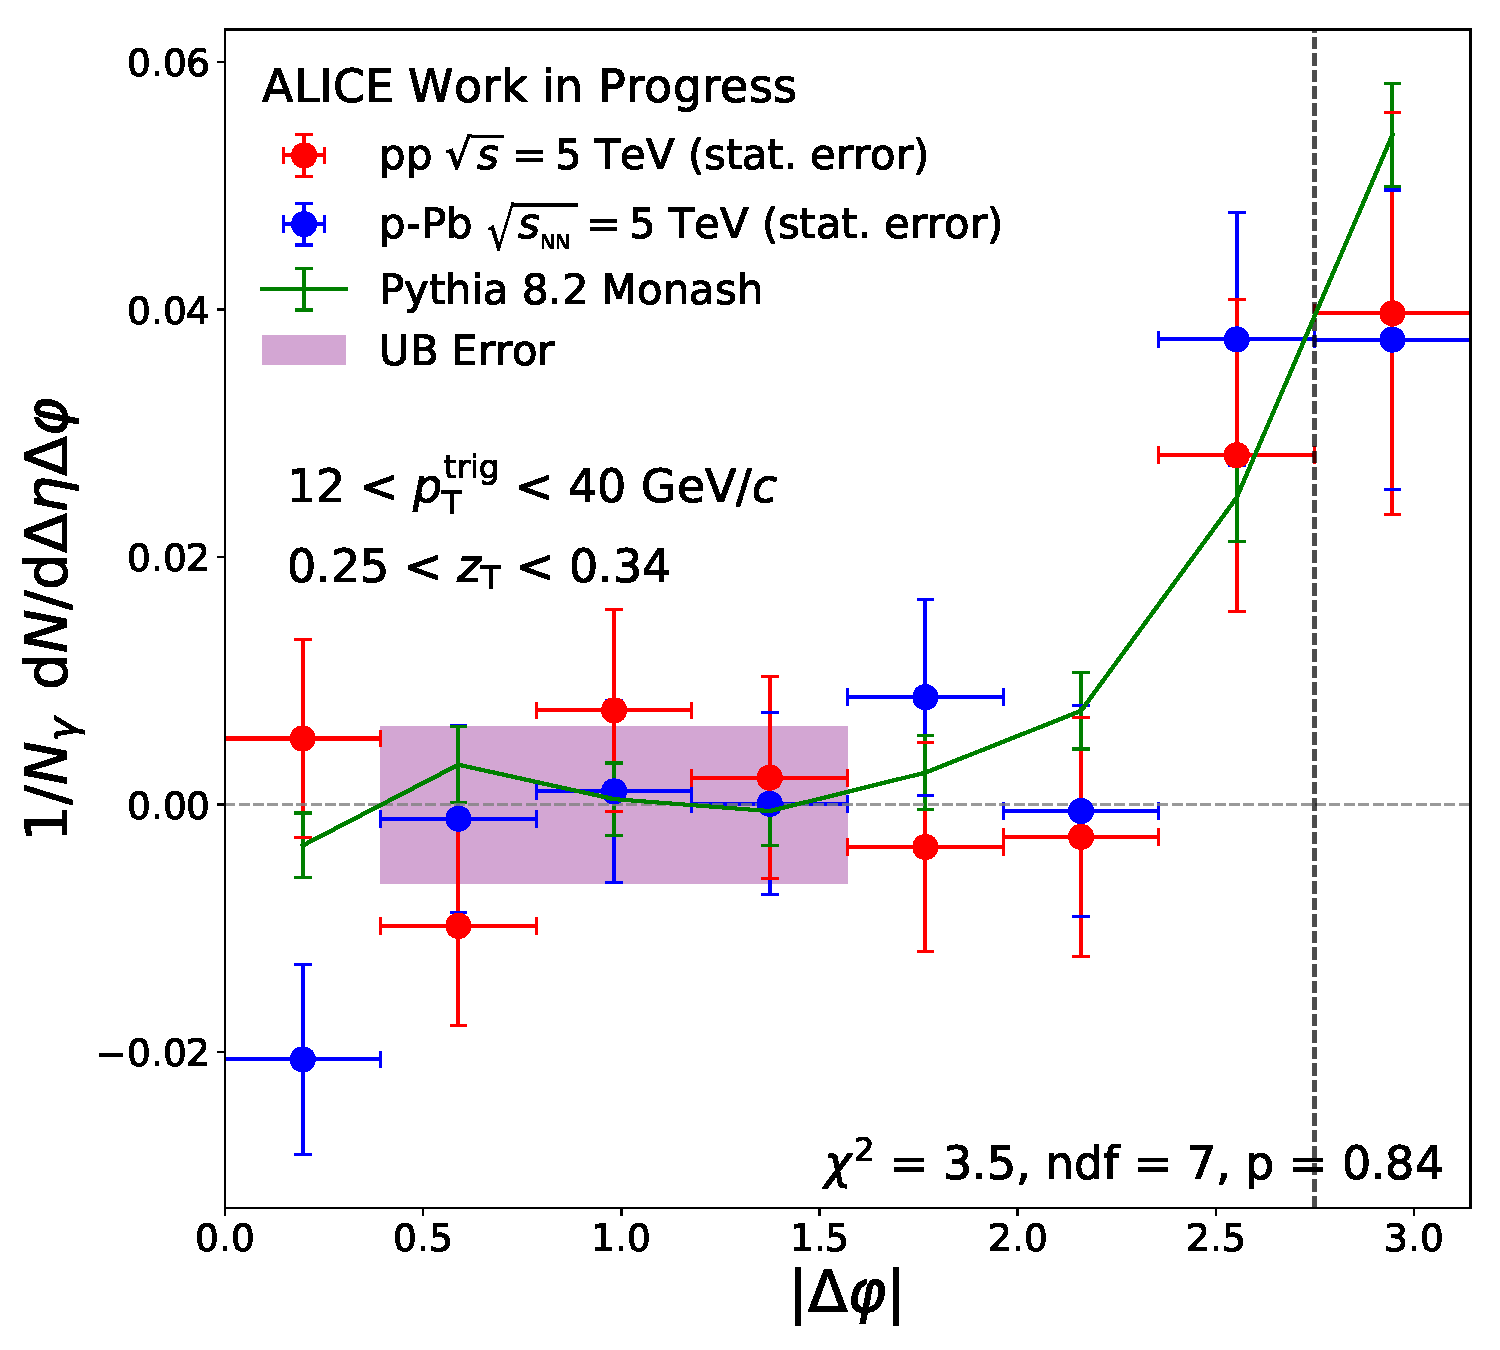
\includegraphics[width = 0.24 \textwidth]{G-H_New/dPhi_to_0/Cs_Final_Indv_pT_0_zT_5.pdf}
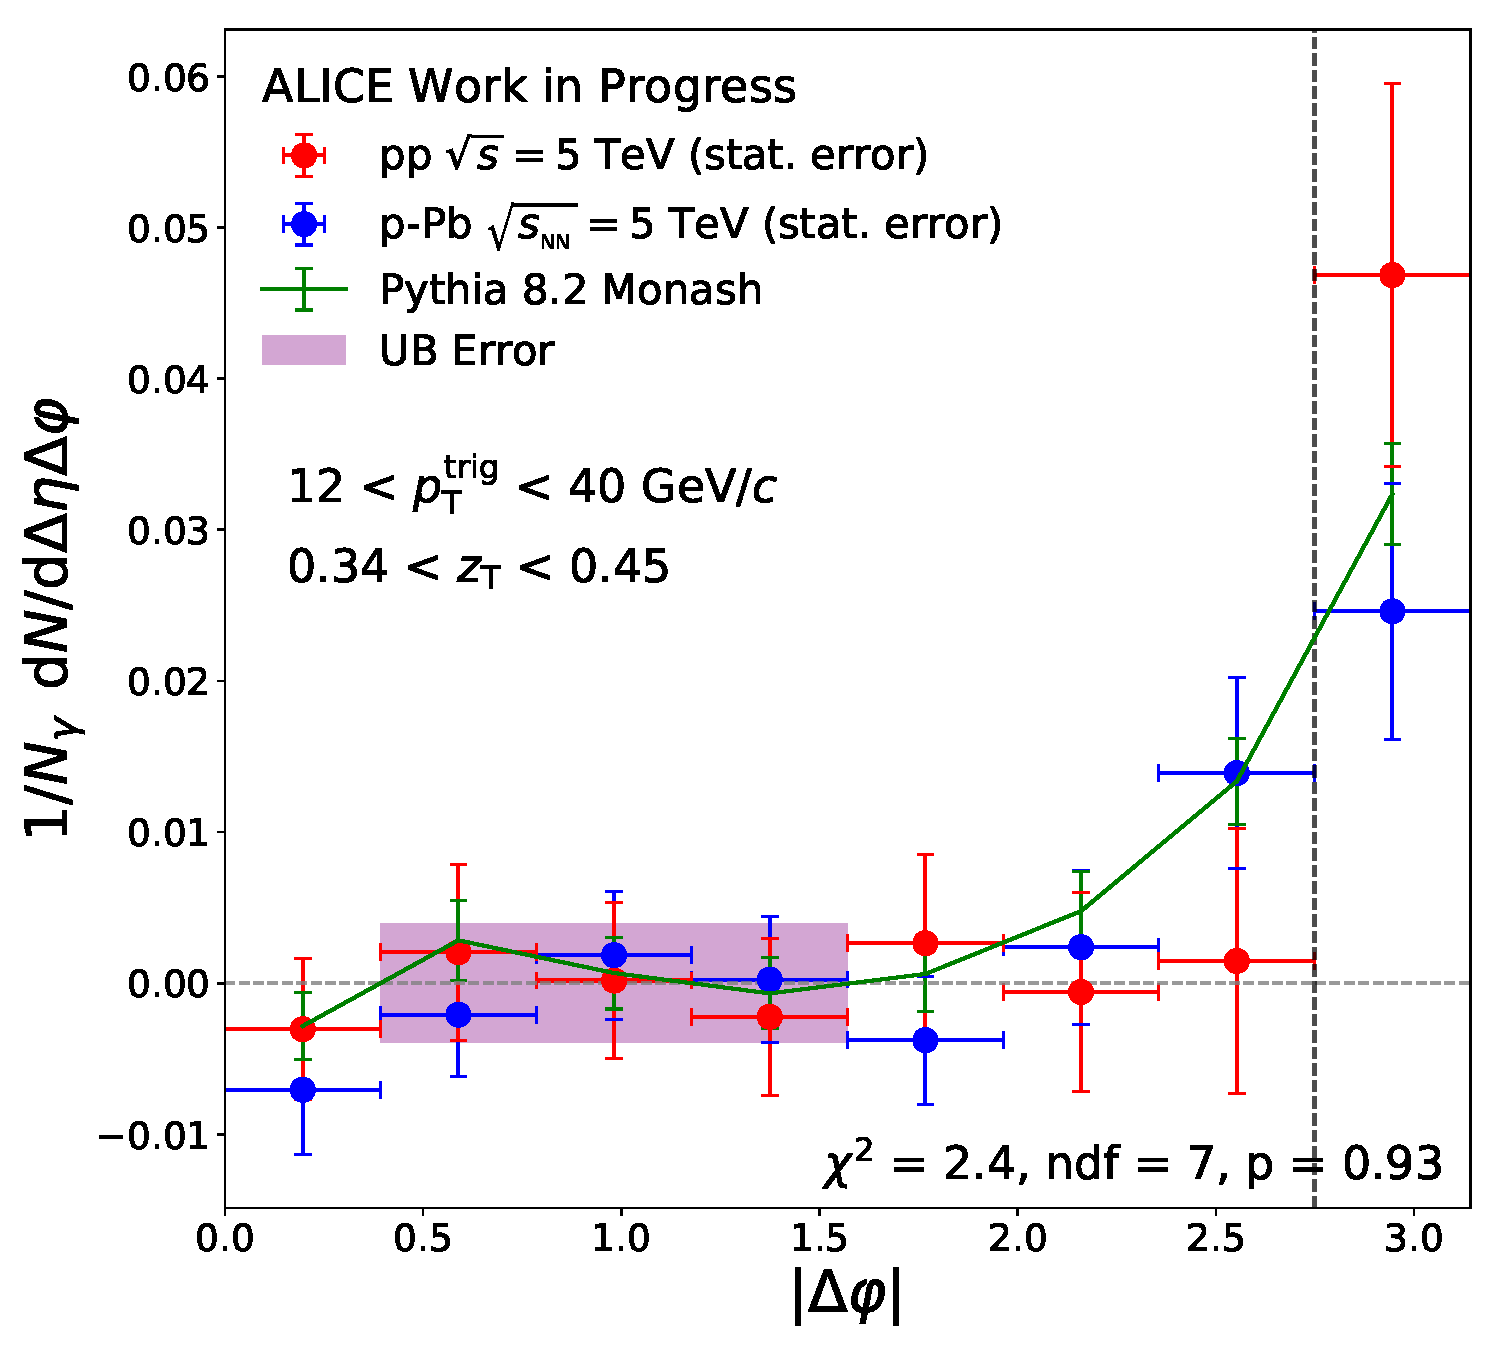
\includegraphics[width = 0.24 \textwidth]{G-H_New/dPhi_to_0/Cs_Final_Indv_pT_0_zT_6.pdf}
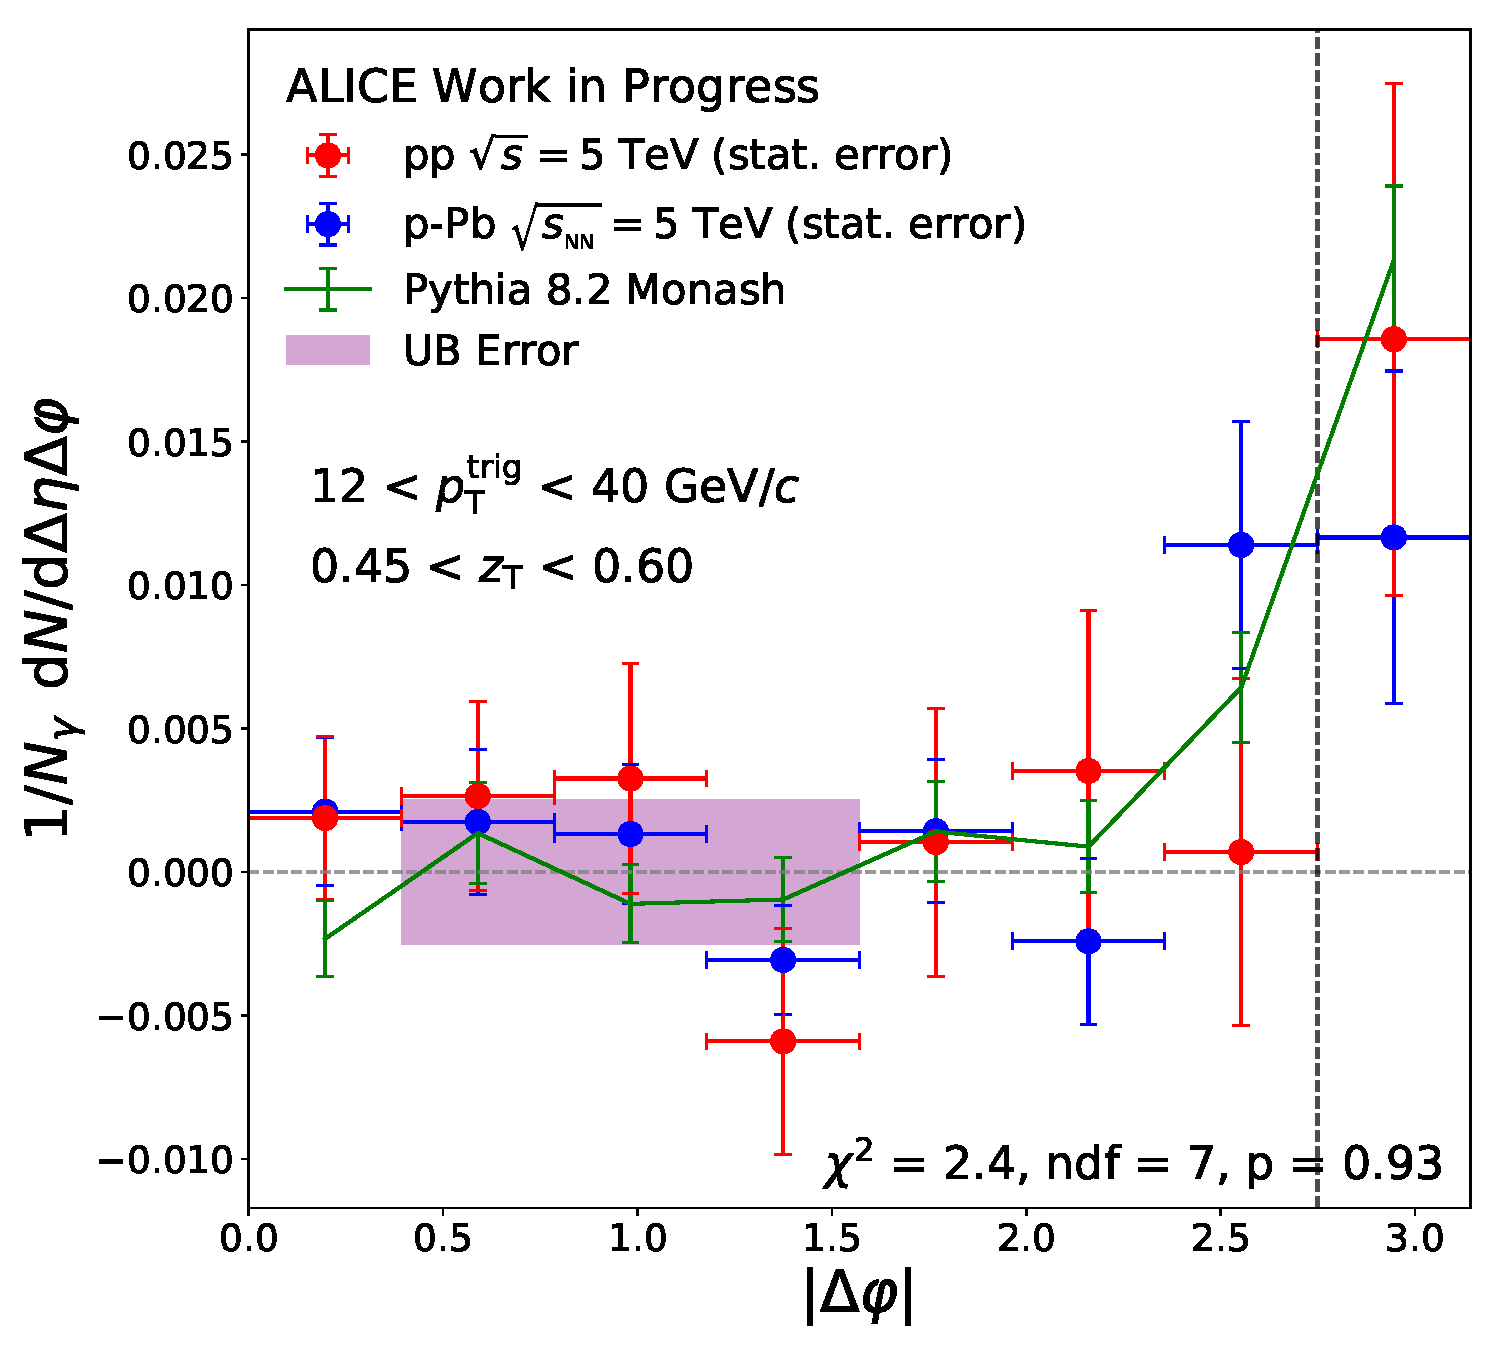
\includegraphics[width = 0.24 \textwidth]{G-H_New/dPhi_to_0/Cs_Final_Indv_pT_0_zT_7.pdf}
\caption{Fully-corrected $\gammaiso$--hadron correlation function pp (red) and \pPb~(blue) data. Identical to Figure \ref{fig:CorrelationFinal} with the exception that we show the correlations down to $\Delta\varphi$=0. }
\label{fig:CorrelationFinal_downtozero}
\end{sidewaysfigure}

%\begin{sidewaysfigure}
%\label{fig:dPhivariation}
%\centering
%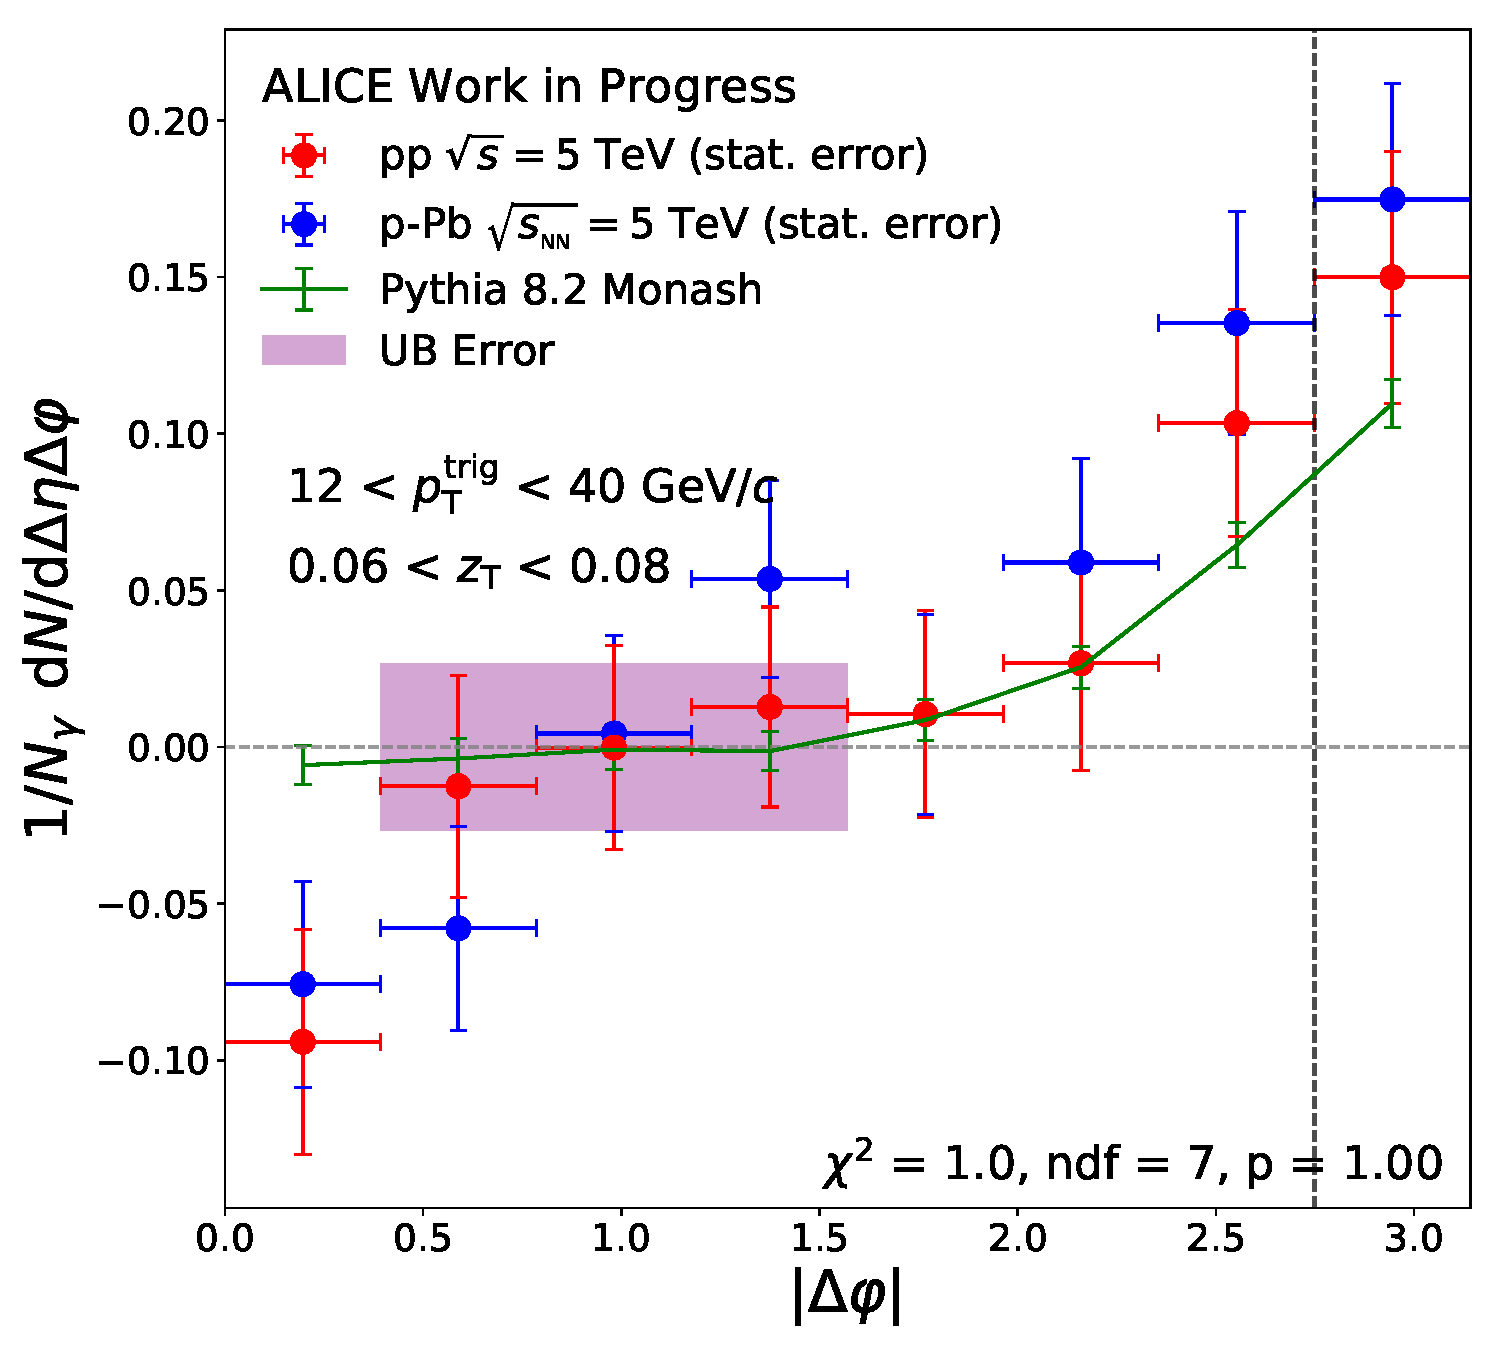
\includegraphics[width = 0.24 %\textwidth]{G-H_New/dPhi_to_0/Cs_Final_Indv_pT_0_zT_0.pdf}
%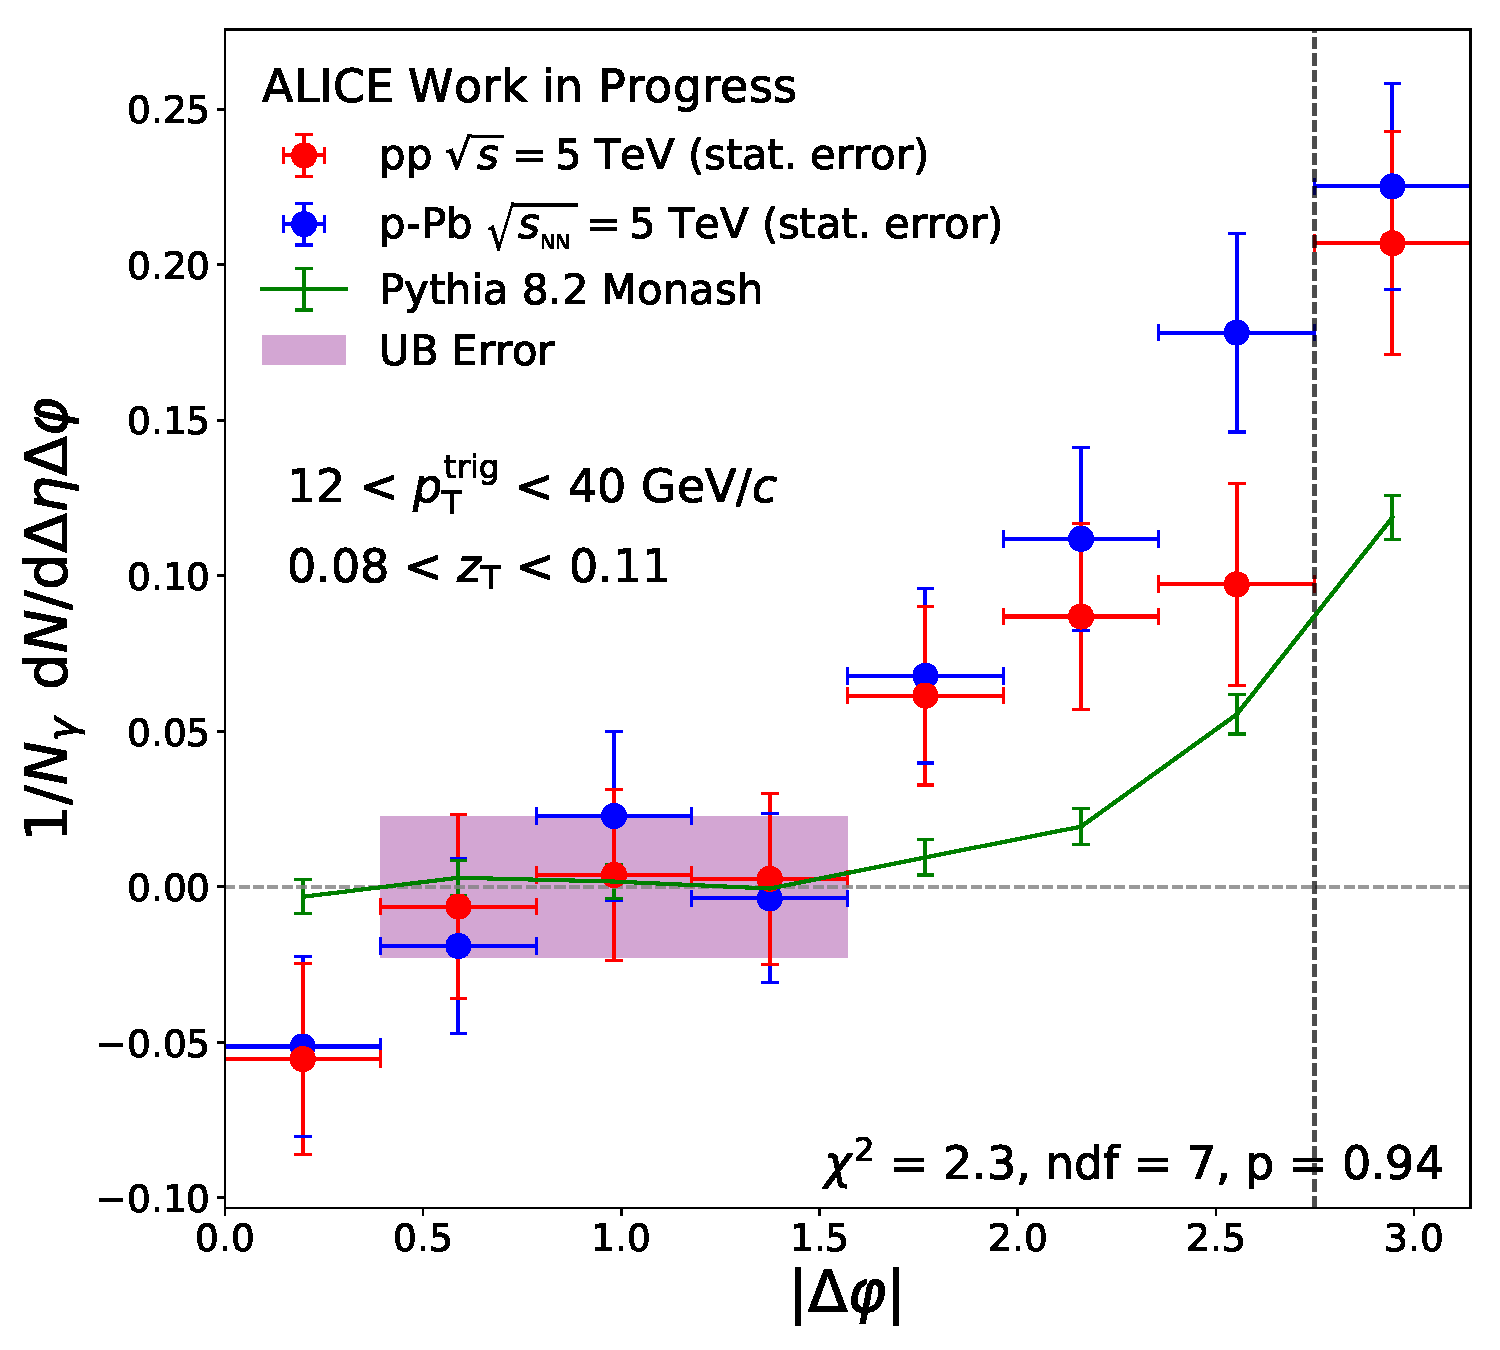
\includegraphics[width = 0.24 %\textwidth]{G-H_New/dPhi_to_0/Cs_Final_Indv_pT_0_zT_1.pdf}
%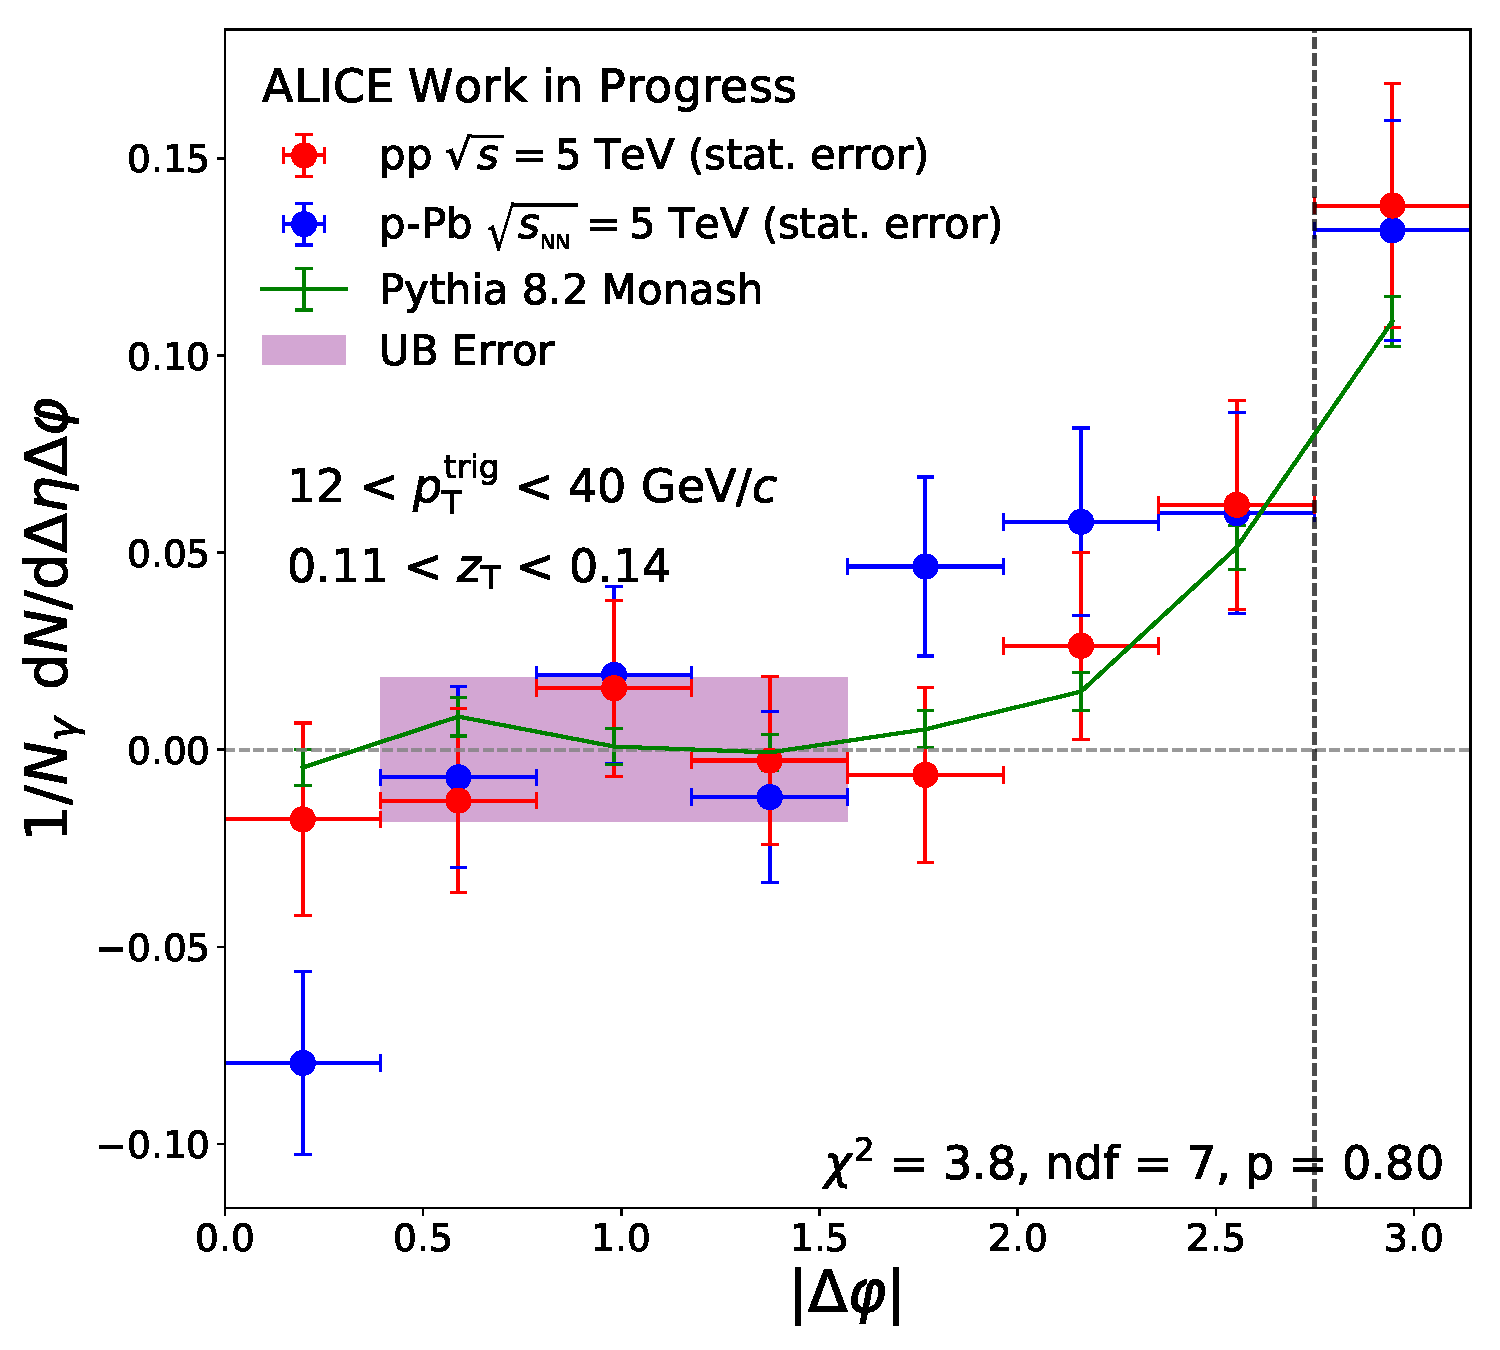
\includegraphics[width = 0.24 %\textwidth]{G-H_New/dPhi_to_0/Cs_Final_Indv_pT_0_zT_2.pdf}
%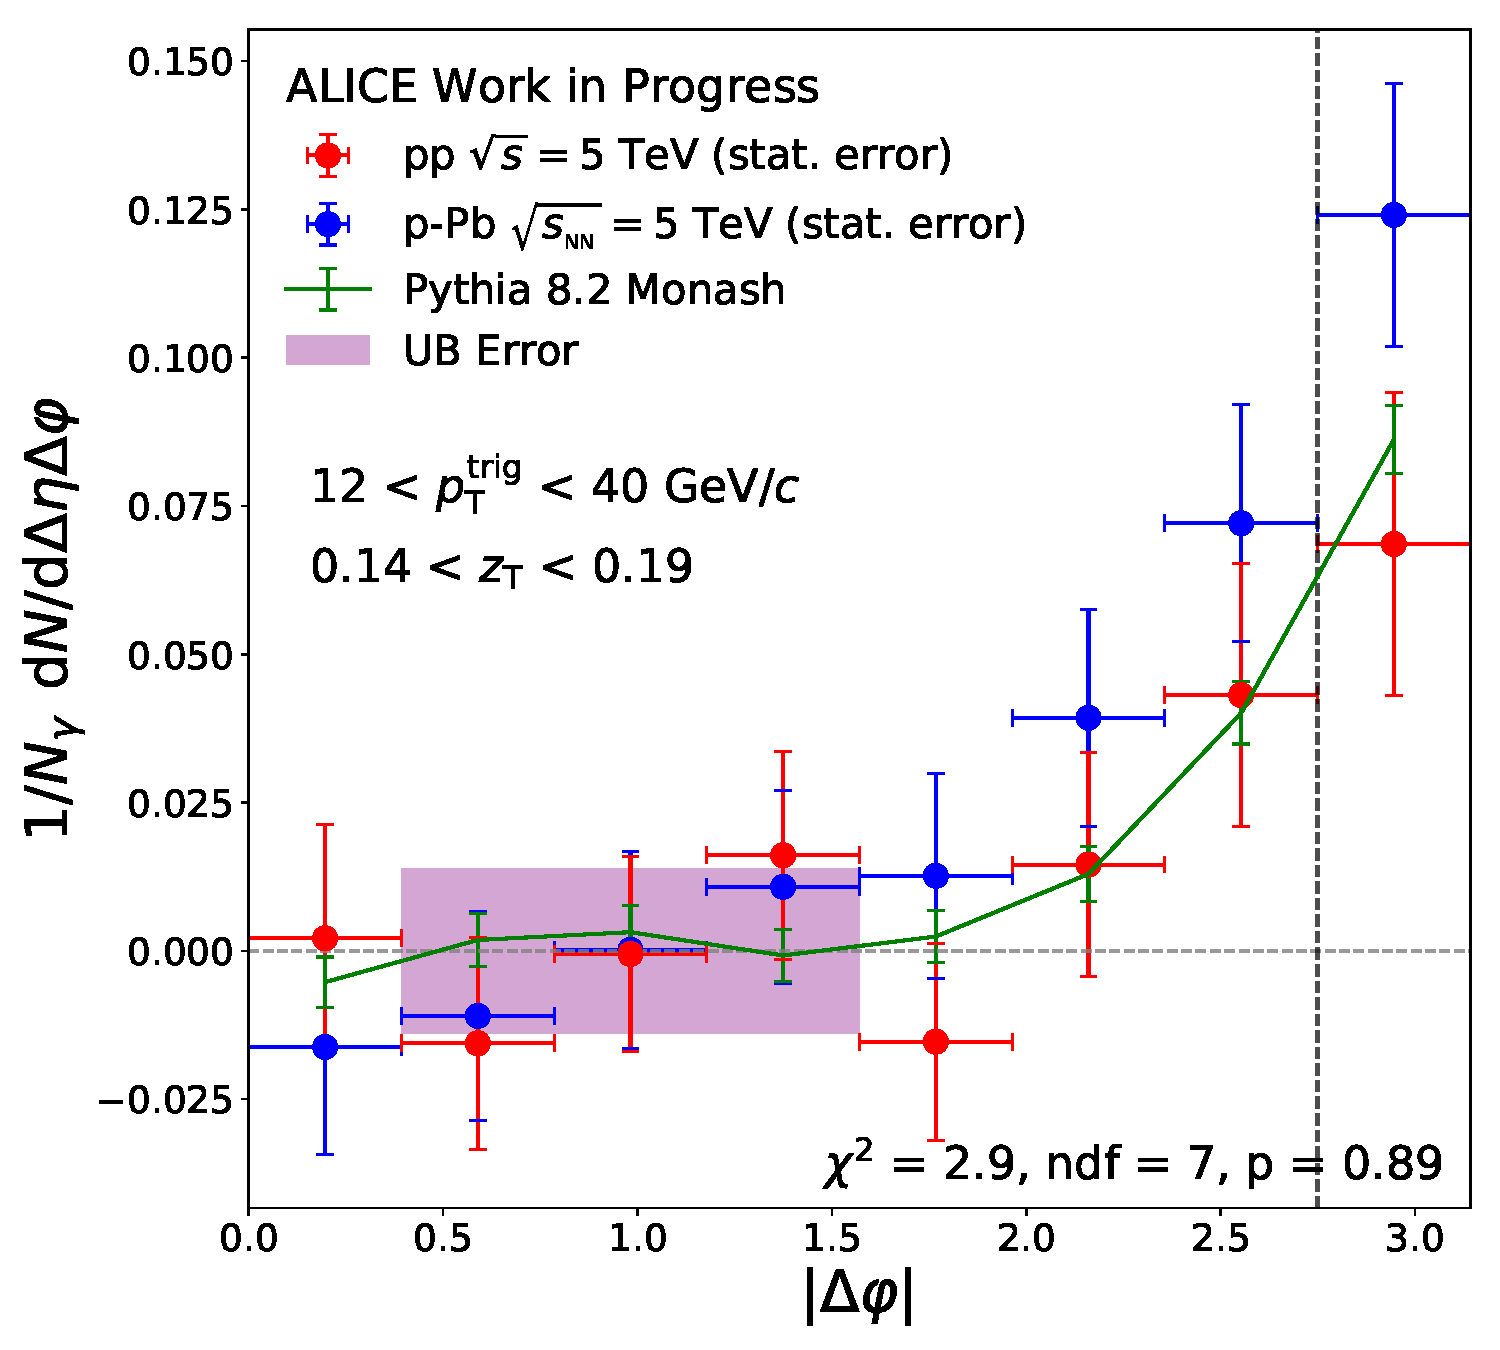
\includegraphics[width = 0.24 %\textwidth]{G-H_New/dPhi_to_0/Cs_Final_Indv_pT_0_zT_3.pdf}
%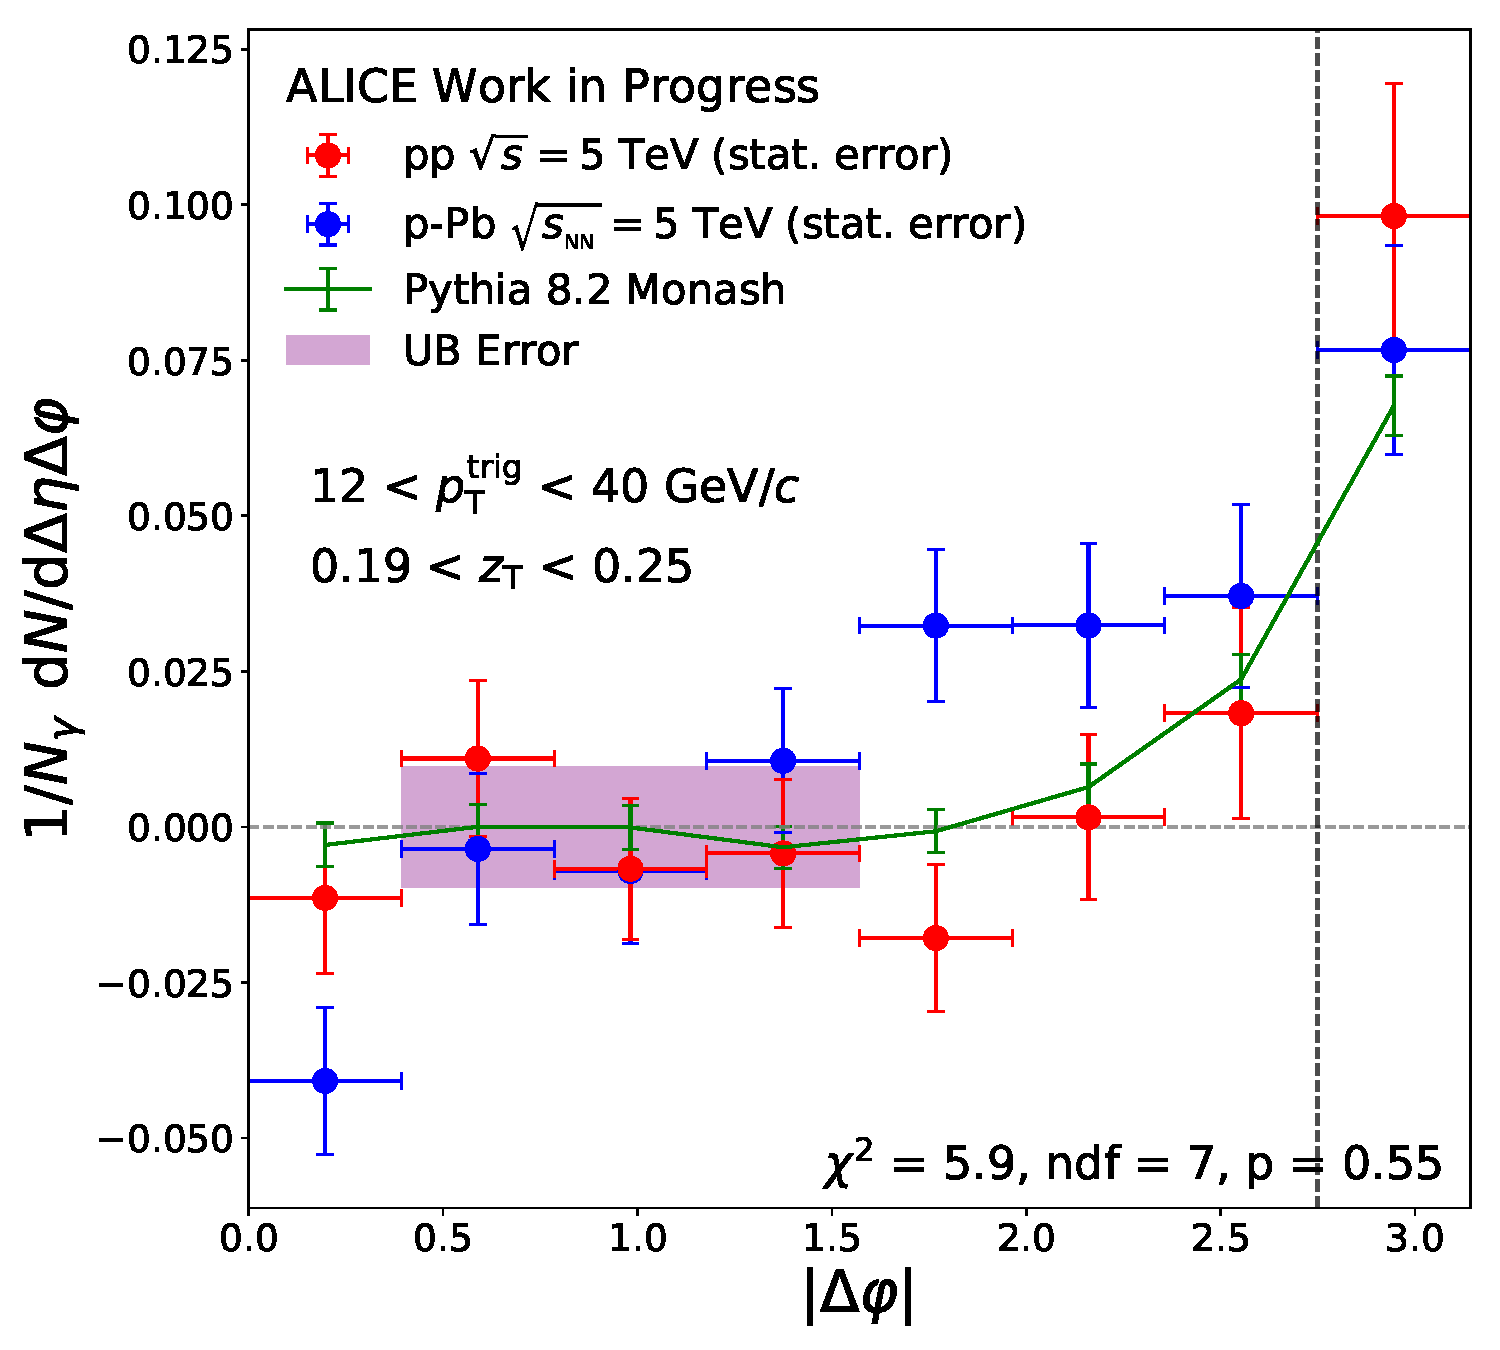
\includegraphics[width = 0.24 \textwidth]{G-H_New/dPhi_to_0/Cs_Final_Indv_pT_0_zT_4.pdf}
%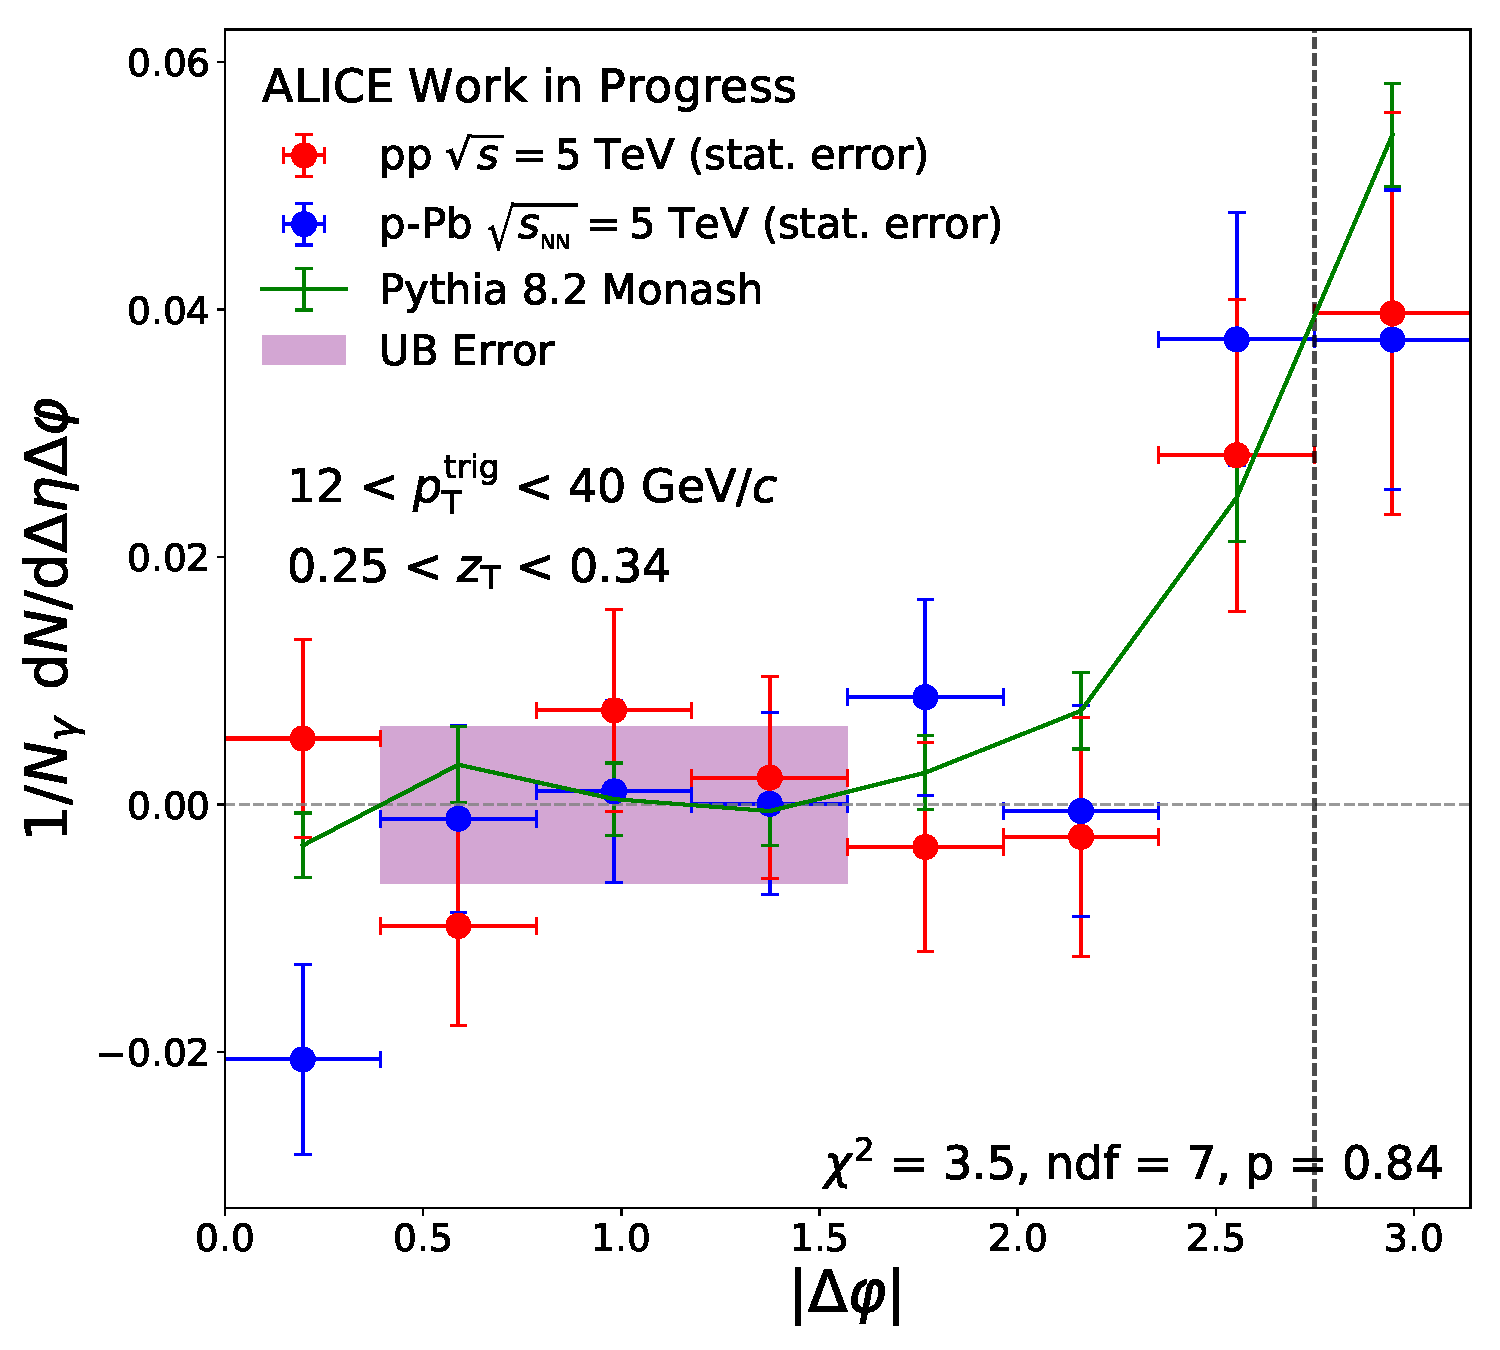
\includegraphics[width = 0.24 \textwidth]{G-H_New/dPhi_to_0/Cs_Final_Indv_pT_0_zT_5.pdf}
%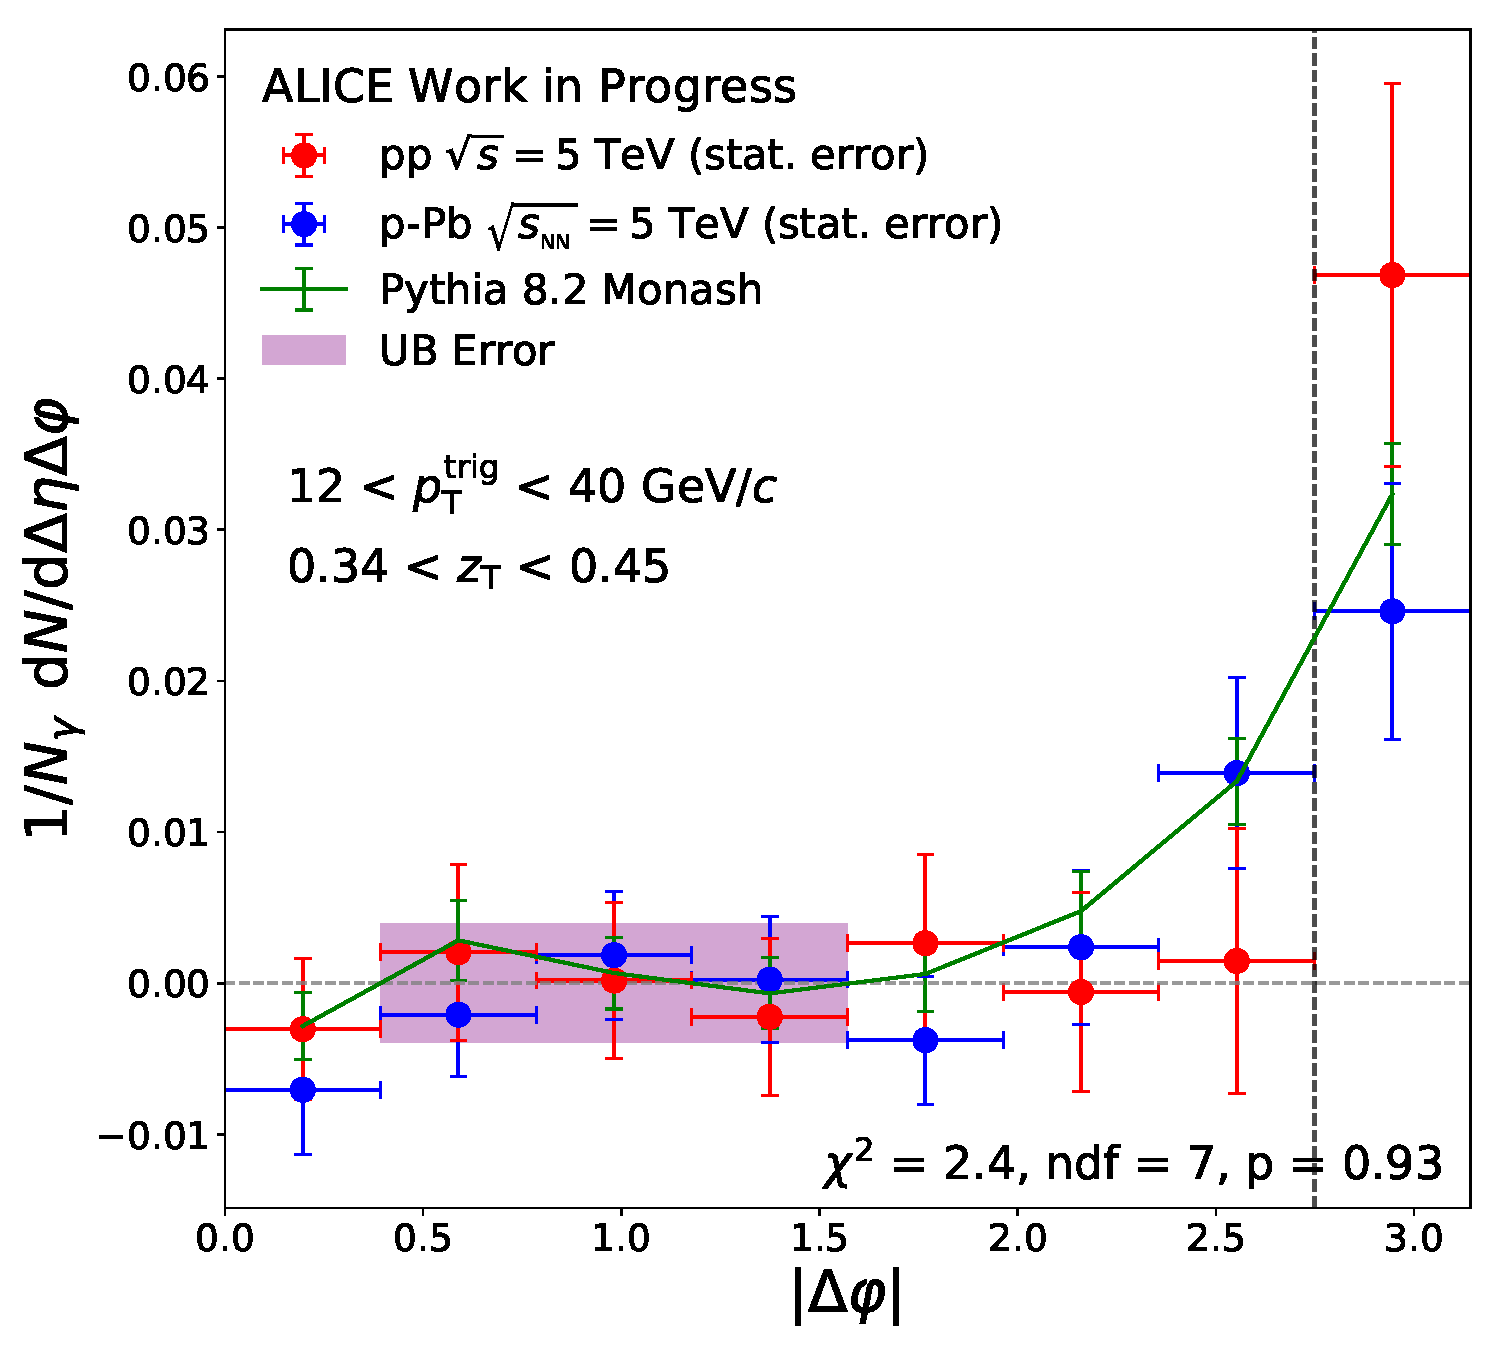
\includegraphics[width = 0.24 %\textwidth]{G-H_New/dPhi_to_0/Cs_Final_Indv_pT_0_zT_6.pdf}
%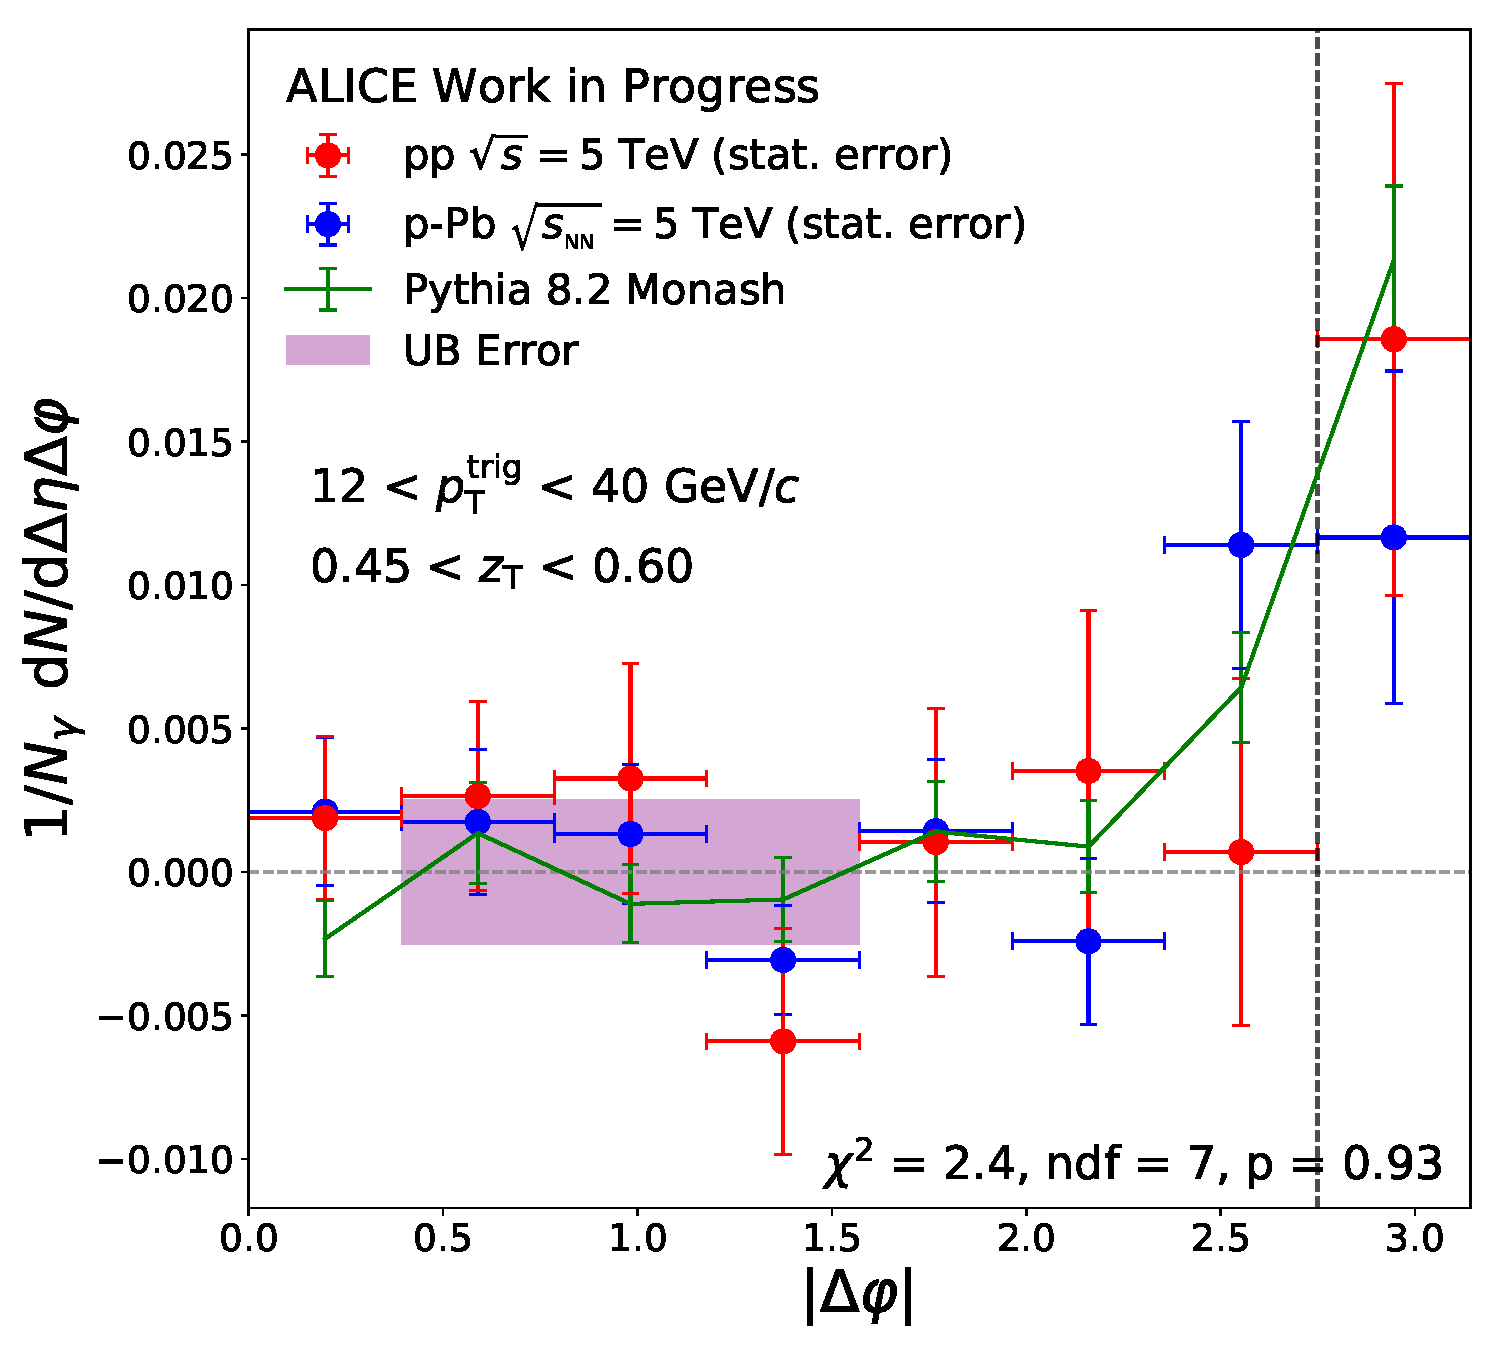
\includegraphics[width = 0.24 %\textwidth]{G-H_New/dPhi_to_0/Cs_Final_Indv_pT_0_zT_7.pdf}
%\caption{Fully-corrected $\gammaiso$--hadron correlation function pp (red) and \pPb~(blue) data. The purple band represents the uncertainty from the underlying event estimate in pp and \pPb. The error bars represent statistical uncertainty only. The green line is the \gammaiso--hadron correlation function obtained with \textsc{PYTHIA 8.2}. This difference with the nominal results shown in Section~\ref{sec:results} is that here we double the number of $\Delta\varphi$ bins.}
%\end{sidewaysfigure}

\section{Comparing ITS only tracking to ITS+TPC Tracking}

Here we show a comparison of results obtained using hybrid (ITS + TPC) tracks in the triggered 13def data (\pPb). Other than the change in the appropriate tracking corrections, the analysis chain is identical to the one that uses our ITS-only tracking. Figure \ref{fig:TPC_CorrelationFinal} shows the correlation functions for \pPb~that uses hybrid tracks and pp which only uses ITS tracks (the TPC was not read out during the 17q data taking).

\begin{sidewaysfigure}
\centering
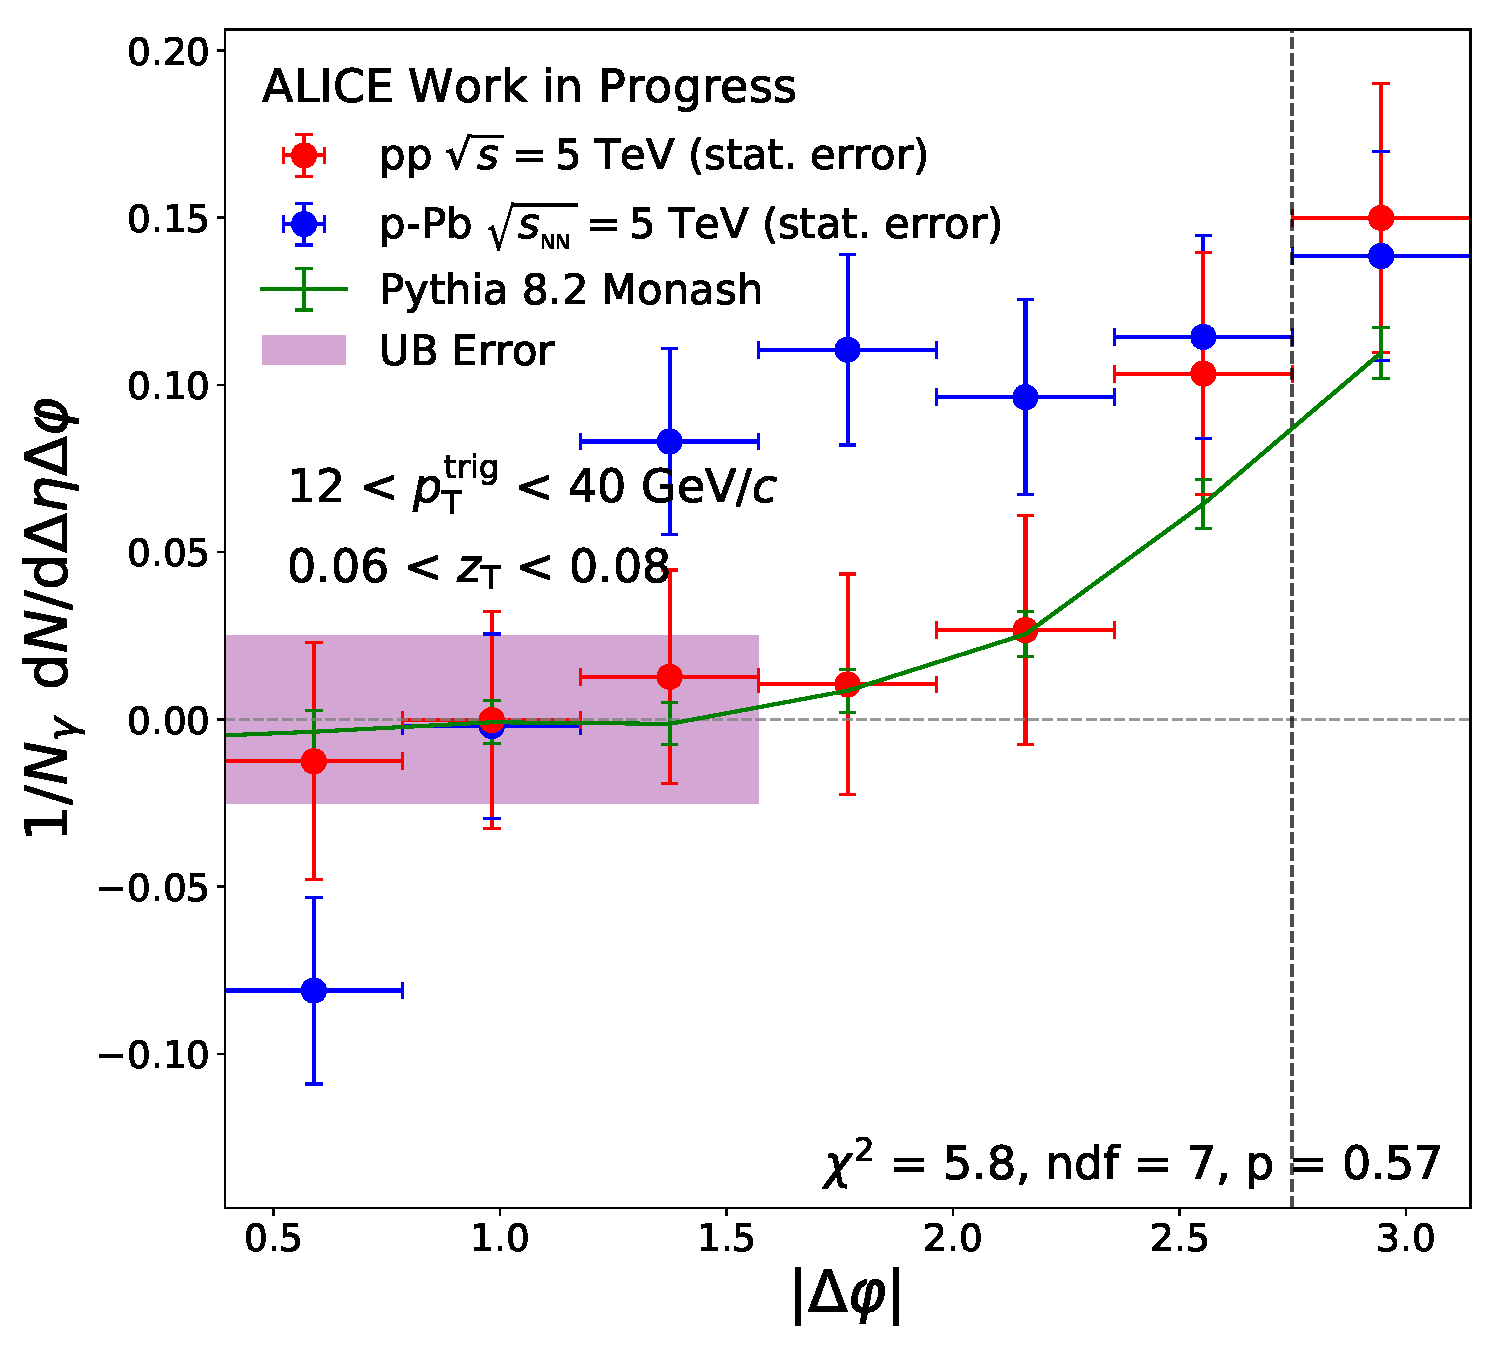
\includegraphics[width = 0.24 \textwidth]{G-H_New/TPC_Tracks/Cs_Final_Indv_pT_0_zT_0.pdf}
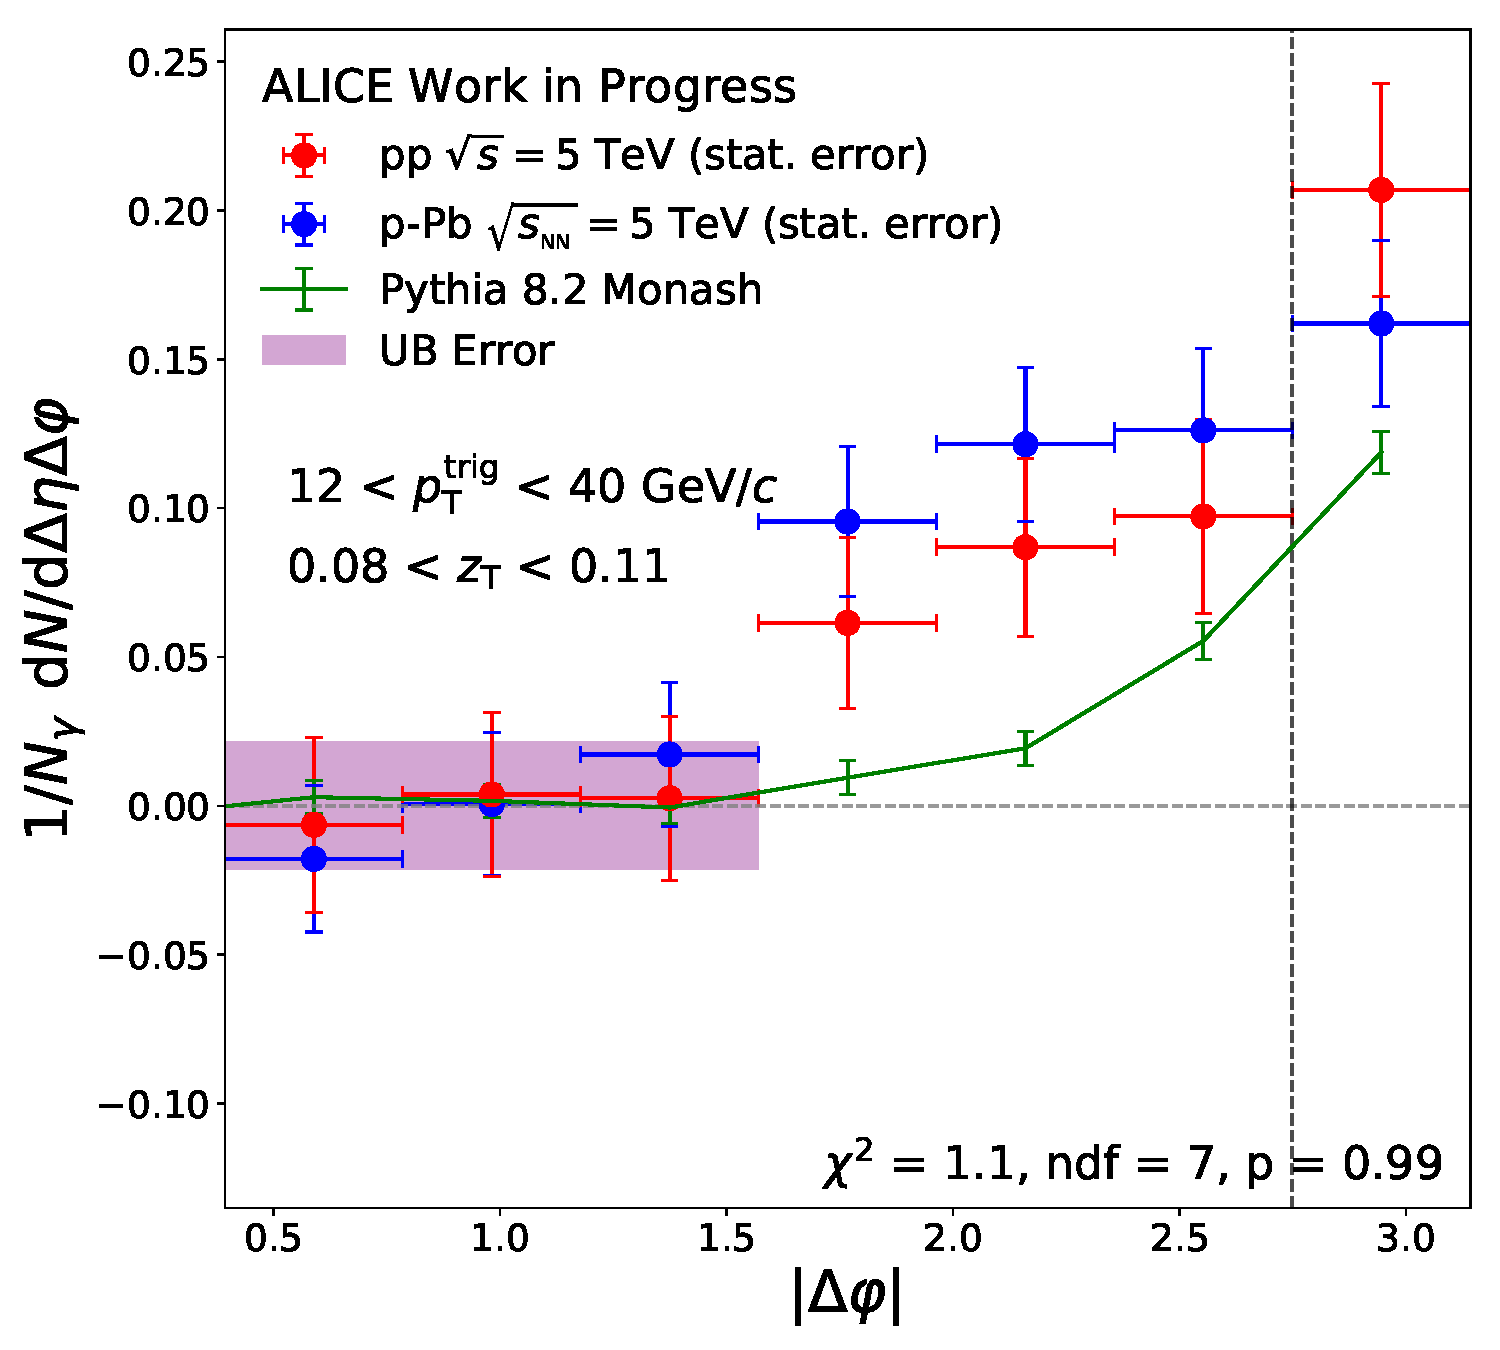
\includegraphics[width = 0.24 \textwidth]{G-H_New/TPC_Tracks/Cs_Final_Indv_pT_0_zT_1.pdf}
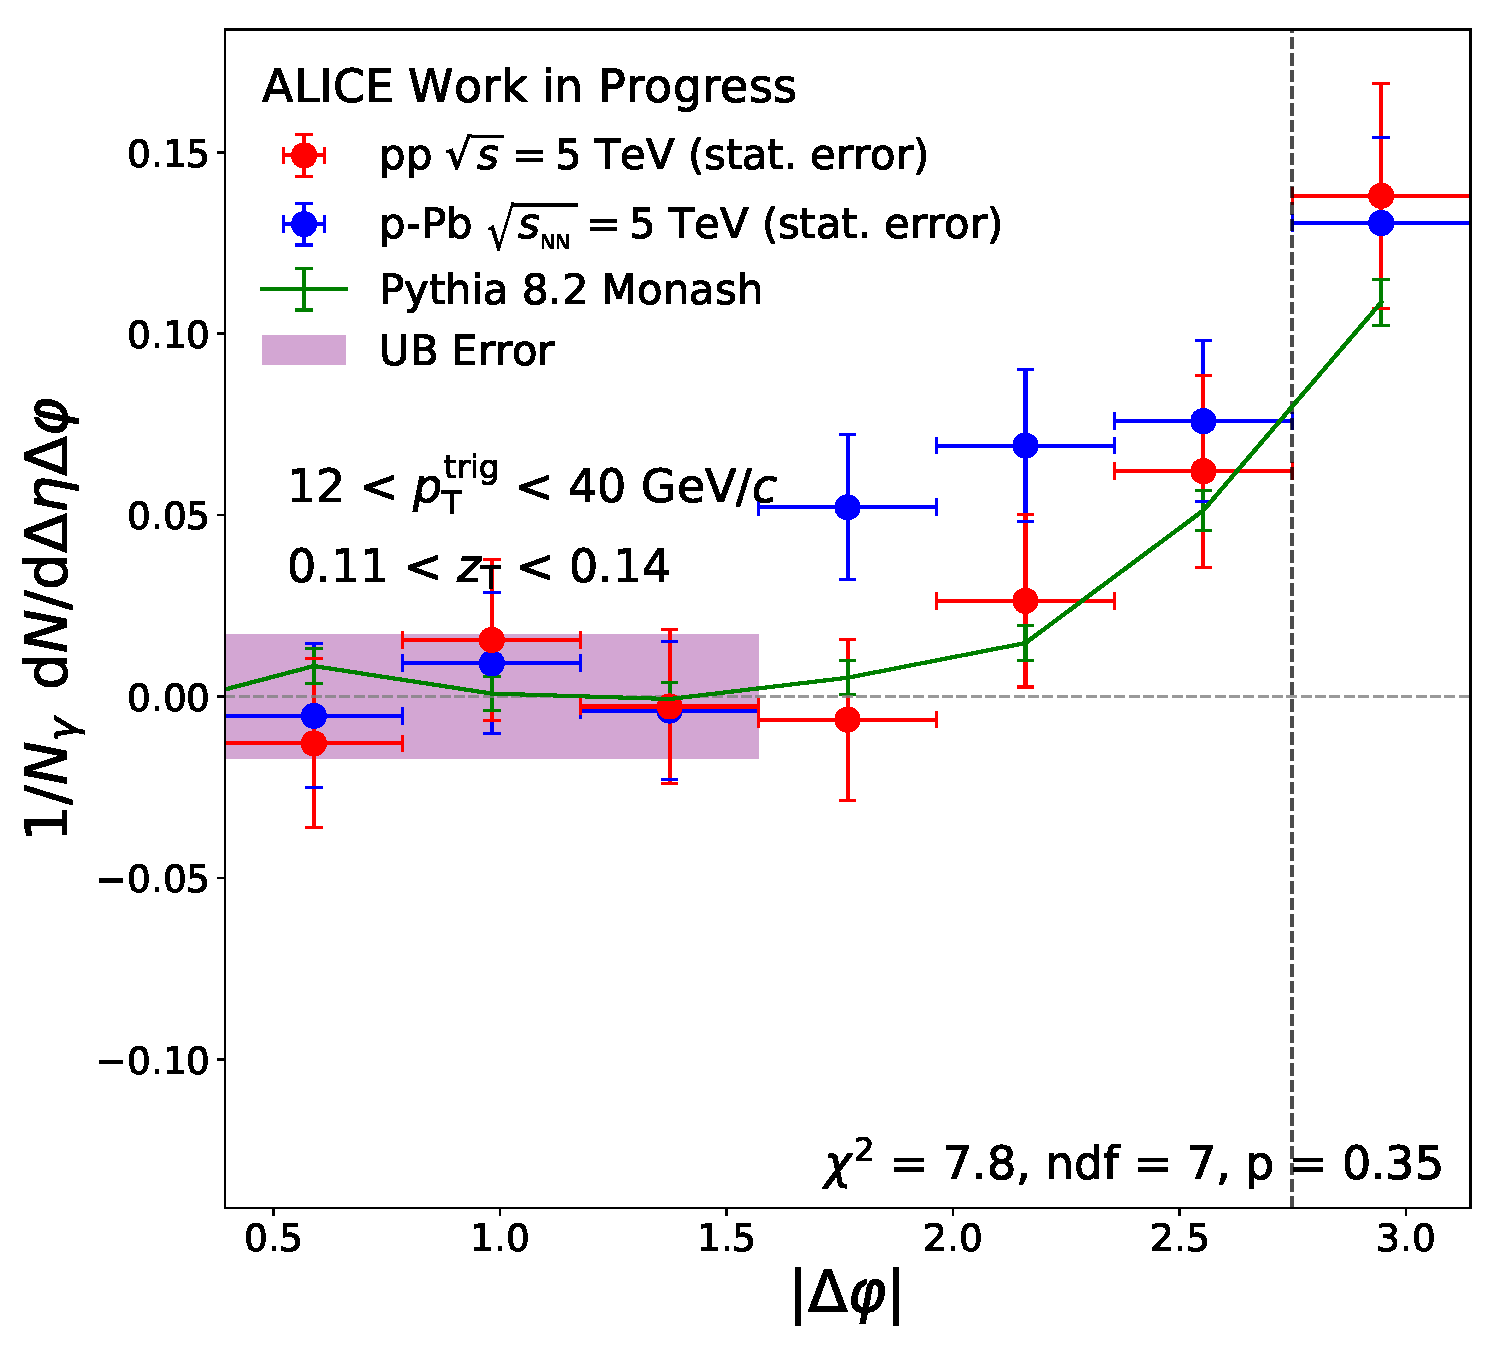
\includegraphics[width = 0.24 \textwidth]{G-H_New/TPC_Tracks/Cs_Final_Indv_pT_0_zT_2.pdf}
\includegraphics[width = 0.24 \textwidth]{G-H_New/TPC_Tracks/Cs_Final_Indv_pT_0_zT_3.pdf}
\includegraphics[width = 0.24 \textwidth]{G-H_New/TPC_Tracks/Cs_Final_Indv_pT_0_zT_4.pdf}
\includegraphics[width = 0.24 \textwidth]{G-H_New/TPC_Tracks/Cs_Final_Indv_pT_0_zT_5.pdf}
\includegraphics[width = 0.24 \textwidth]{G-H_New/TPC_Tracks/Cs_Final_Indv_pT_0_zT_6.pdf}
\includegraphics[width = 0.24 \textwidth]{G-H_New/TPC_Tracks/Cs_Final_Indv_pT_0_zT_7.pdf}
\caption{Fully-corrected $\gammaiso$--hadron correlation function in pp using ITS only tracks (red) and \pPb~ using hybrid tracks (blue).}
\label{fig:TPC_CorrelationFinal}
\end{sidewaysfigure}

\begin{figure}
\centering
\includegraphics[width = 0.49 \textwidth]{G-H_New/TPC_Tracks/Final_FFunction_and_Ratio.pdf}
\includegraphics[width = 0.49 \textwidth]{G-H_New/TPC_Tracks/TPC_Compare_Final_FFunction_and_Ratio.pdf}
\caption{Left: Comparison of final correlations functions for \pPb~Hybrid tracks (blue) and pp ITS only tracks (red). Right: Comparison of final correlations functions for \pPb~Hybrid tracks (red) and \pPb~ITS only tracks (blue).}
\label{fig:TPC_FF}
\end{figure}


Figure \ref{fig:TPC_FF} Shows the fragmentation studies in \pPb~data with ITS only tracks and Hybrid tracks. We can see in the ratio of ITS Only/ Hybrid that the hybrid tracks have a significantly lower yield at high \zt, which roughly corresponds to tracks with high \pt. This is unsurprising as there are issues with TPC charge distortions that have been documented at length [https://alice.its.cern.ch/jira/browse/ATO-351].
\section{Checking sensitivity to $\zt$ binning}
Figure \ref{fig:FF_zT_Rebin} shows the resulting fragmentation function in 6 $zt$ bins. The conclusion we draw from the data does is not affected by this change.


\begin{figure}
\centering
\includegraphics[width=0.49\textwidth]{G-H_New/zT_Rebin_6_006zT06zTITSSub/Final_FFunction_and_Ratio.pdf}
\label{fig:FF_zT_Rebin}
\caption{Results with variation of numbers of \zt~bins. }
\end{figure}


%\FloatBarrier

%\section{Checking sensitivity to pile up cut in pp}
%In this section we apply a stringent pile up cut in our pp dataset. Figure \ref{fig:Correlation_pileup} shows the correlation functions in 6 $\zt$ bins to compensate for the loss of statistics in pp after applying the cut.

%\begin{sidewaysfigure}
%\centering
%\includegraphics[width = 0.32 \textwidth]{G-H_New/zT_Rebin_6_006zT06zTpileCut/Cs_Final_Indv_pT_0_zT_0.pdf}
%\includegraphics[width = 0.32 \textwidth]{G-H_New/zT_Rebin_6_006zT06zTpileCut/Cs_Final_Indv_pT_0_zT_1.pdf}
%\includegraphics[width = 0.32 \textwidth]{G-H_New/zT_Rebin_6_006zT06zTpileCut/Cs_Final_Indv_pT_0_zT_2.pdf}
%\includegraphics[width = 0.32 \textwidth]{G-H_New/zT_Rebin_6_006zT06zTpileCut/Cs_Final_Indv_pT_0_zT_3.pdf}
%\includegraphics[width = 0.32 \textwidth]{G-H_New/zT_Rebin_6_006zT06zTpileCut/Cs_Final_Indv_pT_0_zT_4.pdf}
%\includegraphics[width = 0.32 \textwidth]{G-H_New/zT_Rebin_6_006zT06zTpileCut/Cs_Final_Indv_pT_0_zT_5.pdf}

%\caption{Fully-corrected $\gammaiso$--hadron correlation function in pp (red) and \pPb~(blue) data with the pile up cut in pp only. The correlations have been rebinned to 6 zT bins to compensate for the loss in statistics after applying the cut.}
%\label{fig:Correlation_pileup}
%\end{sidewaysfigure}

%\begin{figure}
%\includegraphics[width=0.49\textwidth]{G-H_New/zT_Rebin_6_006zT06zTpileCut/Final_FFunction_and_Ratio.pdf}
%\label{fig:FF_pileup}
%\end{figure}


%Figure \ref{fig:FF_pileup} shows the resulting fragmentation function in 6 $zt$ bins with the pile up cut applied to the pp data. The figure shows no significant change as a result of this cut.


\section{Checking Maximum Track $\pt$ Cut}
In this section we show the effect of varying the maximum $\pt$ cut on the final away-side yields in pp and \pPb. We then show the effect this variation has on the final ratio.

\begin{figure}
\includegraphics[width=0.49\textwidth]{G-H_New/FF_Averages_Max_pT_pp.pdf}
\includegraphics[width=0.49\textwidth]{G-H_New/Ratio_FF_Averages_Max_pT.pdf}
\caption{Left: The away side yields in pp with a maximum $p_\mathrm{T}^\mathrm{Track}$ cut of 10,8, and 6 GeV/$c$. Right: The Ratio of \pPb~to pp with a maximum $p_\mathrm{T}^\mathrm{Track}$ cut of 10,8, and 6 GeV/$c$}
\label{fig:FF_pT_Max_pp}
\end{figure}


\section{Purity result with newly reconstructed data}

Figure~\ref{newpurity} shows the purity measurement we obtain with the newly reconstructed 13f data. The measurements are compatible within statistical variations. 

\begin{figure}
\centering
\includegraphics[width=0.5\textwidth]{Purity/purities13ffinal.pdf}
\caption{Nominal results for purity and purity measured with the newly reconstructed 13f runs.}
\label{newpurity}
\end{figure}

\section{Sensitivity to $\chi^2/\mathrm{ITS}_{clus}$ in p-Pb}
The effect of the $\chi^2/\mathrm{ITS}_{clus}$ cut on the tracking efficiency, fake rate, and bin migration is studied to select the most effective $\chi^2/\mathrm{ITS}_{clus}$ maximum limit. Four values have been tested: $\chi^2/\mathrm{ITS}_{clus} =$ 1, 2, 3, and 36. The following figures~\ref{fig:chi2_eff}, ~\ref{fig:chi2_fr}, ~\ref{fig:chi2_bm}, and ~\ref{fig:chi2_w} show the effect of $\chi^2/\mathrm{ITS}_{clus}$ cuts on the efficiency, fake rate, bin migration, and track correction weight. The weight is calculated from the efficiency, fake rate, and bin migration using equation~\ref{eq:track_weight}. The efficiency seems to be similar for all cut variation except for $\chi^2/\mathrm{ITS}_{clus}$ < 1, where it is lower by 5\%. However, the fake rate and bin migration effects are improved as the cut is tightened. It is to note that regardless of the threshold for the $\chi^2/\mathrm{ITS}_{clus}$ cut, as long as identical cuts are applied to both the Monte Carlo and the data sets used in the section~\ref{sec:tracking}, the fine agreement with published data is always present.

\begin{figure}[h]
    \centering
    \includegraphics[width=0.49\textwidth]{Appendices/ITSchi2_study_efficiency.pdf}
        \includegraphics[width=0.49\textwidth]{Appendices/ITSchi2_study_fakerate.pdf}
    \caption{Left: The efficiency comparison for the various $\chi^2/\mathrm{ITS}_{clus}$ cuts. Right: The fake rate comparison for the various $\chi^2/\mathrm{ITS}_{clus}$ cuts}
    \label{fig:chi2_eff}
\end{figure}

Additionally, figure~\ref{fig:chi2SpectraComparison} shows the effect of changing the $\chi^2/ITS_{clus}$ from $\chi^2/ITS_{clus} < 36$ to $\chi^2/ITS_{clus} < 3$ on the track \pt spectra as the ratio of $\chi^2/ITS_{clus} <3$ and $\chi^2/ITS_{clus} < 36$. From the top two plots, we can see that the change in the cut does not affect the \pt spectra as the raito is consistent with unity within 5\% up 8 GeV/ as along as the appropriate Monte Carlo anchored to the data is used. However, the bottom plots, uses LHC13def, but corrects using the 13b2 Monte Carlo, and divergence from unity shows the instability of the $\chi^2/ITS_{clus}$ cut. Thus, we have moved from using the 13b2 Monte Carlo to using 17g6a1 to correct the 13def data set.
\begin{figure}[h]
\center
\includegraphics[width=0.46\textwidth]{Appendices/ITSchi2_study_ptSpectra_ratio_MBMB.pdf}
\includegraphics[width=0.46\textwidth]{Appendices/ITSchi2_study_ptSpectra_ratio_MBGJ.pdf}
\includegraphics[width=0.46\textwidth]{Appendices/ITSchi2_study_ptSpectra_ratio_GJGJ.pdf}
\caption{The changes in the tracking spectra with respect to the $\chi^2/ITS_{clus}$ cut. The top left is the 13b data corrected using 13b2 Monte Carlo. The top right is 13def data corrected using 17g6a1 Monte Carlo. And the bottom plot is 13def data corrected using 13b2 Monte Carlo.}
\label{fig:chi2SpectraComparison}
\end{figure}

Finally, we compare the efficiency, fake rate, bin migration and the weights between ITS-only tracking in p-Pb and pp, and TPC+ITS tracking in p-Pb using 17g6a1. We can see all the TPC+ITS and ITS-only tracking are comparable within uncertainties, while the ITS-only pp and p-Pb follow similar shapes. This result agrees with acceptations and trend demonstrated in section~\ref{sec:tracking}. The key difference is that in section~\ref{sec:tracking} all the figures are produced using 13b2, the minimum bias Monte Carlo, while in the case for figure~\ref{fig:TPCITSpp_pPbCompare}, we use 17g6a1, the gamma-jet Monte Carlo. 
\begin{figure}[h]
\center
\includegraphics[width=0.46\textwidth]{Appendices/ITSchi2_study_efficiency.pdf}
\includegraphics[width=0.46\textwidth]{Appendices/ITSchi2_study_fakerate.pdf}
\includegraphics[width=0.46\textwidth]{Appendices/ITSchi2_study_binMigration.pdf}
\includegraphics[width=0.46\textwidth]{Appendices/ITSchi2_study_weight.pdf}
\caption{The comparison of efficiency (top left), fake rate (top right), bin migration (bottom left), and weights (bottom right) between ITS-only tracking for p-Pb and pp, as well as TPC+ITS tracking for p-Pb using the 17g6a1 gamma-jet Monte Carlo.}
\label{fig:TPCITSpp_pPbCompare}
\end{figure}